\subsubsection{Case Description}
%%%%%%%%%%%%%%%%%%%%%%%%%%%%%%%%%%%%%%%%%%%%%%%%%%%%%%%%%%%
\begin{figure}[t]  
\centering
     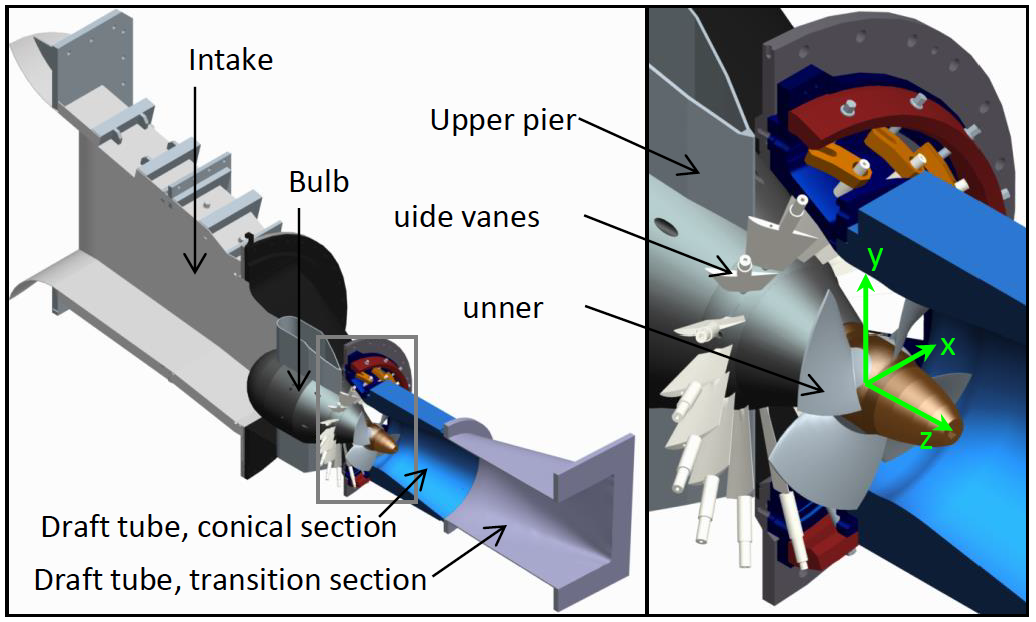
\includegraphics[clip=true, trim= 0.0cm 0.0cm 0.0cm 0.0cm,width=0.99\linewidth]{./figures/bulbt/bulbt}                            
     \caption{Turbine model of BulbT \cite{vuillemard2014experimental}.}
     \label{bulbt}
\end{figure} 
%%%%%%%%%%%%%%%%%%%%%%%%%%%%%%%%%%%%%%%%%%%%%%%%%%%%%%%%%%%
\begin{figure}[t] 
\centering
     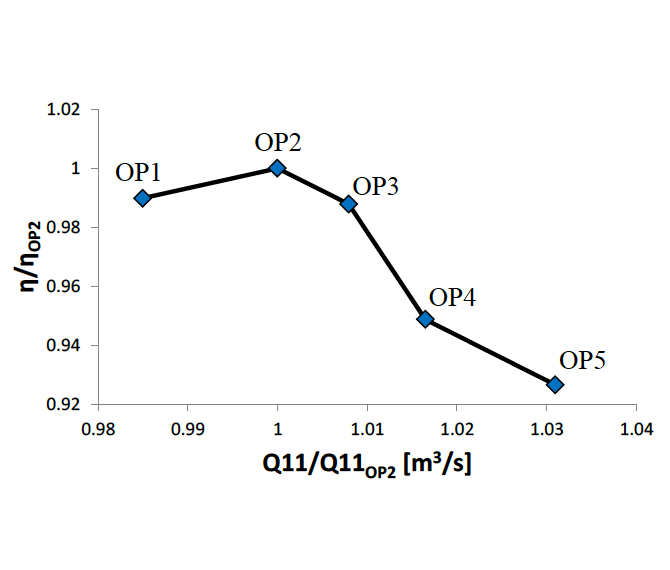
\includegraphics[clip=true, trim= 0.0cm 3.0cm 0.0cm 3.0cm,width=0.99\linewidth]{./figures/bulbt/bulbt-op}                  
     \caption{Operating points of BulbT \cite{vuillemard2014experimental}.}
     \label{bulbt-op}
\end{figure}
%%%%%%%%%%%%%%%%%%%%%%%%%%%%%%%%%%%%%%%%%%%%%%%%%%%%%%%%%%%
The BulbT project was initiated at the ``Laboratoire de Machines Hydrauliques'' (LAMH) of Laval University, and aimed at investigating the flow phenomena in a bulb turbine \cite{vu2014cfd}. The turbine model consists of an intake, a bulb and a draft tube, as illustrated in Fig.~\ref{bulbt}. The experiments were conducted at five Operating Points (OP) as shown in Fig.~\ref{bulbt-op}; where OP2 is closest to the best efficiency point (BEP), and the flow phenomenon is less complex compared to other OPs. Therefore, in this work, OP2 is chosen for validating the proposed schemes.
%%%%%%%%%%%%%%%%%%%%%%%%%%%%%%%%%%%%%%%%%%%%%%%%%%%%%%%%%%%
%%%%%%%%%%%%%%%%%%%%%%%%%%%%%%%%%%%%%%%%%%%%%%%%%%%%%%%%%%%
%%%%%%%%%%%%%%%%%%%%%%%%%%%%%%%%%%%%%%%%%%%%%%%%%%%%%%%%%%%
%%%%%%%%%%%%%%%%%%%%%%%%%%%%%%%%%%%%%%%%%%%%%%%%%%%%%%%%%%%
%%%%%%%%%%%%%%%%%%%%%%%%%%%%%%%%%%%%%%%%%%%%%%%%%%%%%%%%%%%
%%%%%%%%%%%%%%%%%%%%%%%%%%%%%%%%%%%%%%%%%%%%%%%%%%%%%%%%%%%
%%%%%%%%%%%%%%%%%%%%%%%%%%%%%%%%%%%%%%%%%%%%%%%%%%%%%%%%%%%
\begin{figure}[t]  
\centering
     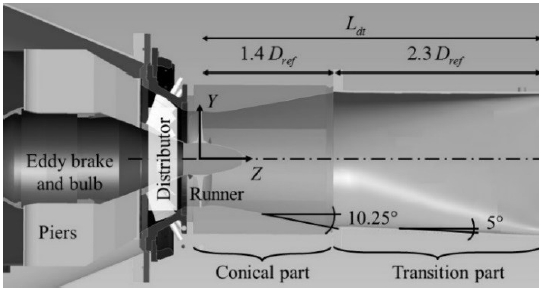
\includegraphics[clip=true, trim= 0.0cm 0.0cm 0.0cm 0.0cm,width=0.99\linewidth]{./figures/bulbt/drafttube}                            
     \caption{Geometry of the draft tube \cite{pereira2017flow}.}
     \label{drafttube}
\end{figure}
%%%%%%%%%%%%%%%%%%%%%%%%%%%%%%%%%%%%%%%%%%%%%%%%%%%%%%%%%%%

The geometry of the draft tube is shown in Fig.~\ref{drafttube}. The draft tube is composed of two parts, a conical and a transition part. The conical part has a divergence angle of $10.25^{\circ}$ and a length of 1.4 times the diameter of the runner shroud, $D_{ref}$. The transition part transforms the cross section from a circular shape to a rectangular shape. It has a length of  $2.3D_{ref}$ and it is not symmetric. The divergence angles are $9.5^{\circ}$ on the left and right sides, and $5^{\circ}$ on the bottom side, while the top side is near horizontal.
%%%%%%%%%%%%%%%%%%%%%%%%%%%%%%%%%%%%%%%%%%%%%%%%%%%%%%%%%%%
%%%%%%%%%%%%%%%%%%%%%%%%%%%%%%%%%%%%%%%%%%%%%%%%%%%%%%%%%%%
%%%%%%%%%%%%%%%%%%%%%%%%%%%%%%%%%%%%%%%%%%%%%%%%%%%%%%%%%%%
\begin{figure}[t]  
\centering
     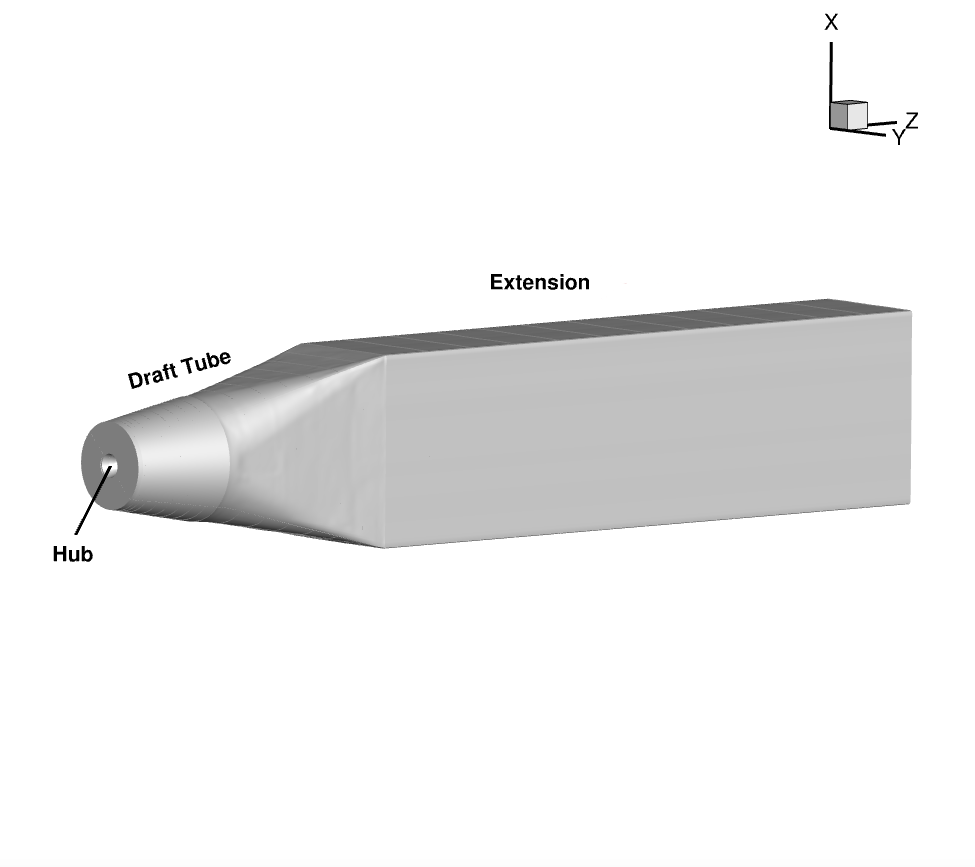
\includegraphics[clip=true, trim= 1.75cm 9.5cm 1.75cm 0.0cm,width=0.99\linewidth]{./figures/bulbt/geometry}                            
     \caption{Geometry of the grid.}
     \label{geometry}
\end{figure}
%%%%%%%%%%%%%%%%%%%%%%%%%%%%%%%%%%%%%%%%%%%%%%%%%%%%%%%%%%%

The numerical simulations were performed on three consecutively refined grids, which consist of 3M, 14M and 50M cells respectively. The grid only consists of the hub, the draft tube and an extension as shown in Fig.~\ref{geometry}. The extension is added to ensure that the flow discharges to the reservoir at ambient conditions. A sideview, and the inlet and outlet of the 14M grid are shown in Fig.~\ref{grid1}. In Fig.~\ref{grid2}, the zoom-in view illustrates that central regions downstream of the hub and near-wall regions are refined, in order to better capture the flow features. The first cells close to the wall are placed at $y^{+}\approx 1$ for all three grids.
\begin{figure*}[t]  
\centering
     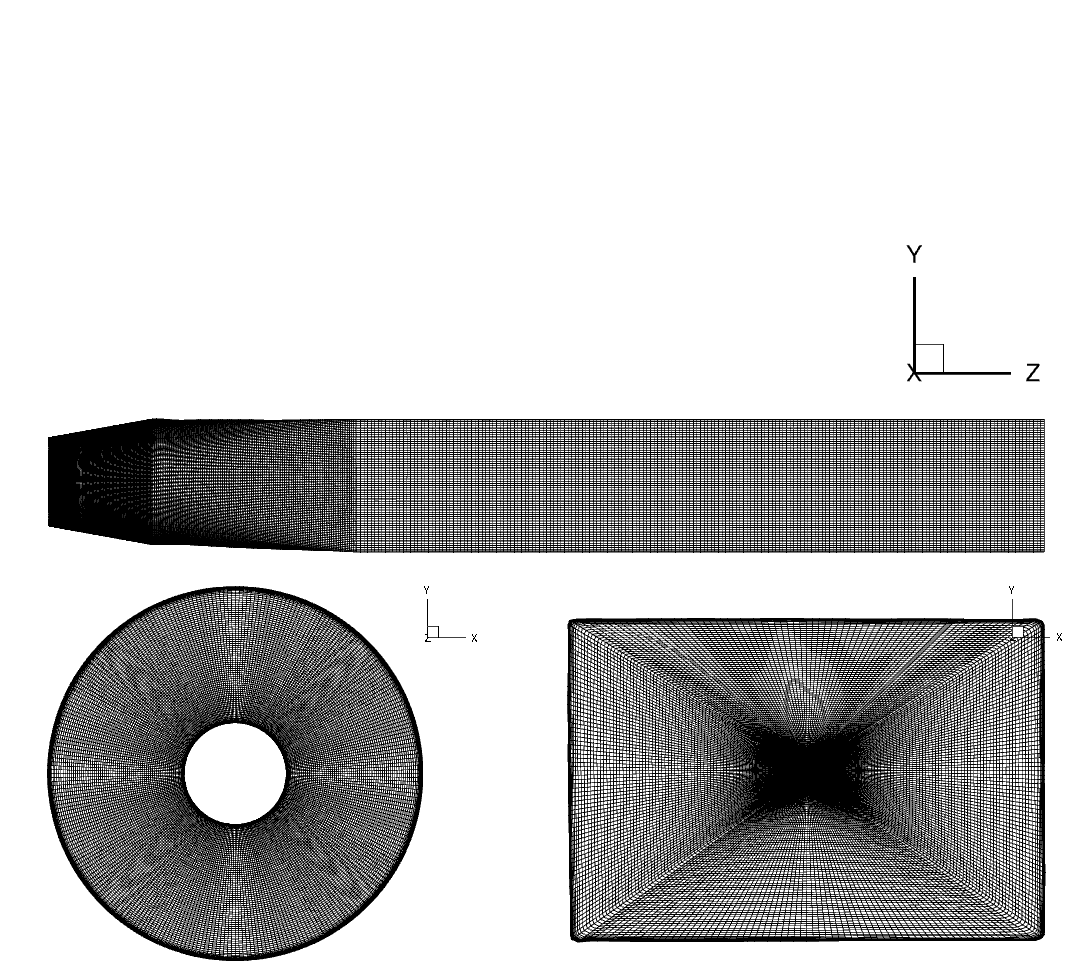
\includegraphics[clip=true, trim= 0.0cm 0.0cm 0.0cm 8.0cm,width=0.99\linewidth]{./figures/bulbt/grid/overview}                            
     \caption{Overview of the 14M grid.}
     \label{grid1}
\end{figure*}
%%%%%%%%%%%%%%%%%%%%%%%%%%%%%%%%%%%%%%%%%%%%%%%%%%%%%%%%%%%
\begin{figure*}[t]  
\centering
     \subfigure[]{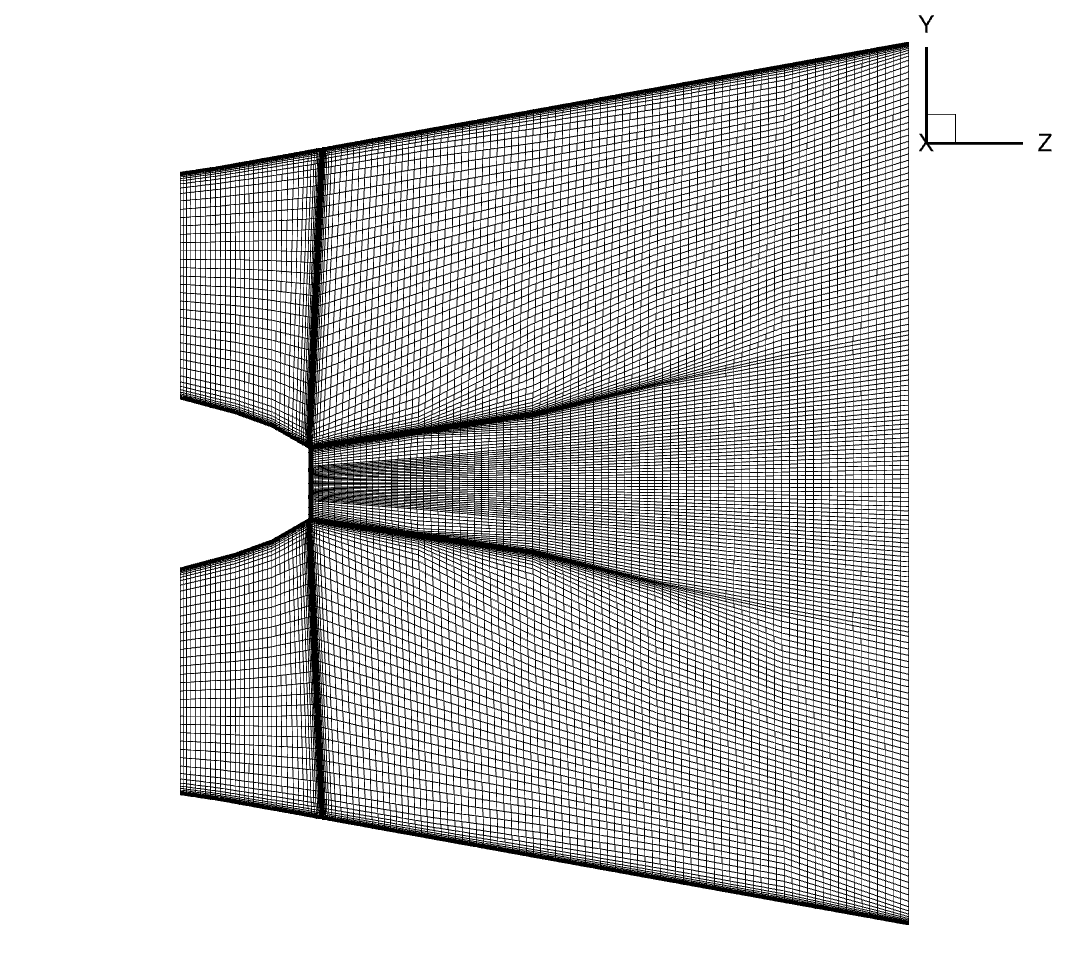
\includegraphics[clip=true, trim= 3.0cm 8.0cm 4.0cm 8.0cm,width=0.325\linewidth]{./figures/bulbt/grid/3m}}          
     \subfigure[]{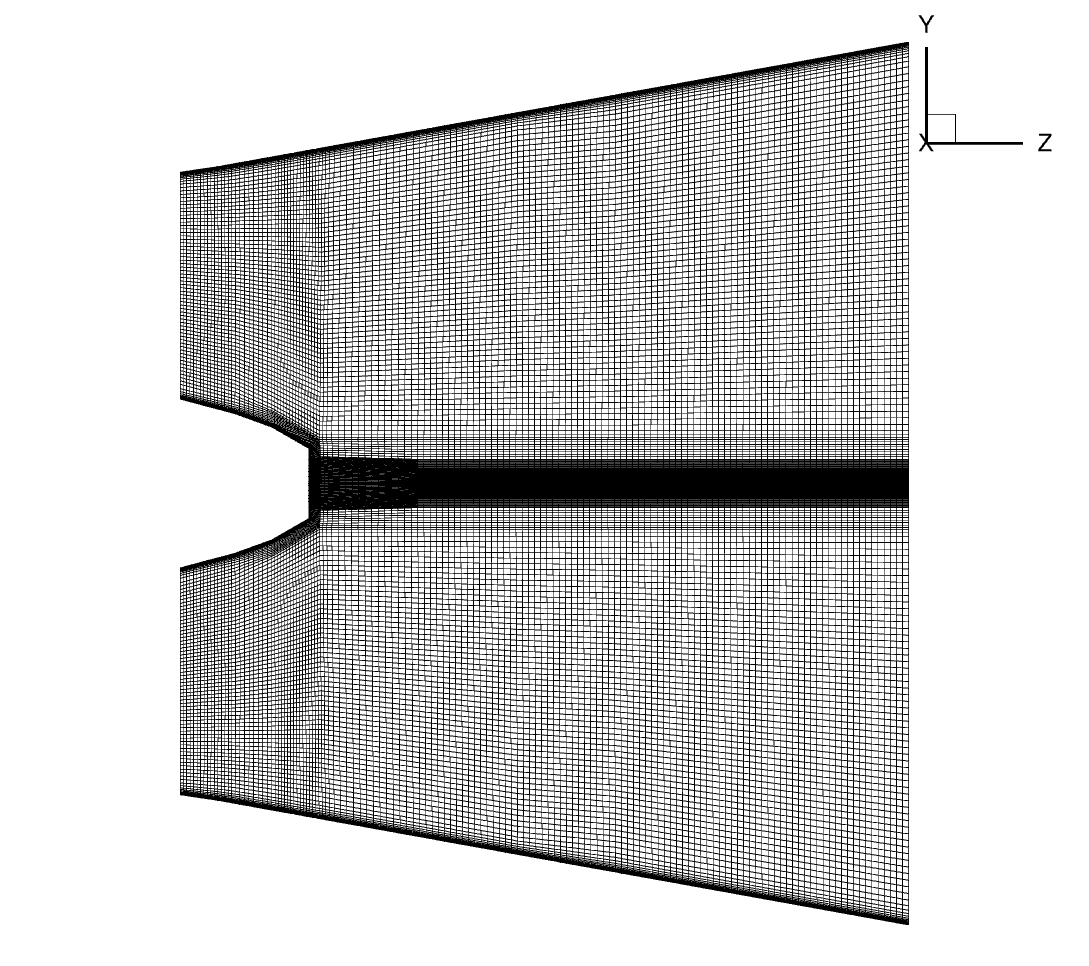
\includegraphics[clip=true, trim= 3.0cm 8.0cm 4.0cm 8.0cm,width=0.325\linewidth]{./figures/bulbt/grid/14m}}       
     \subfigure[]{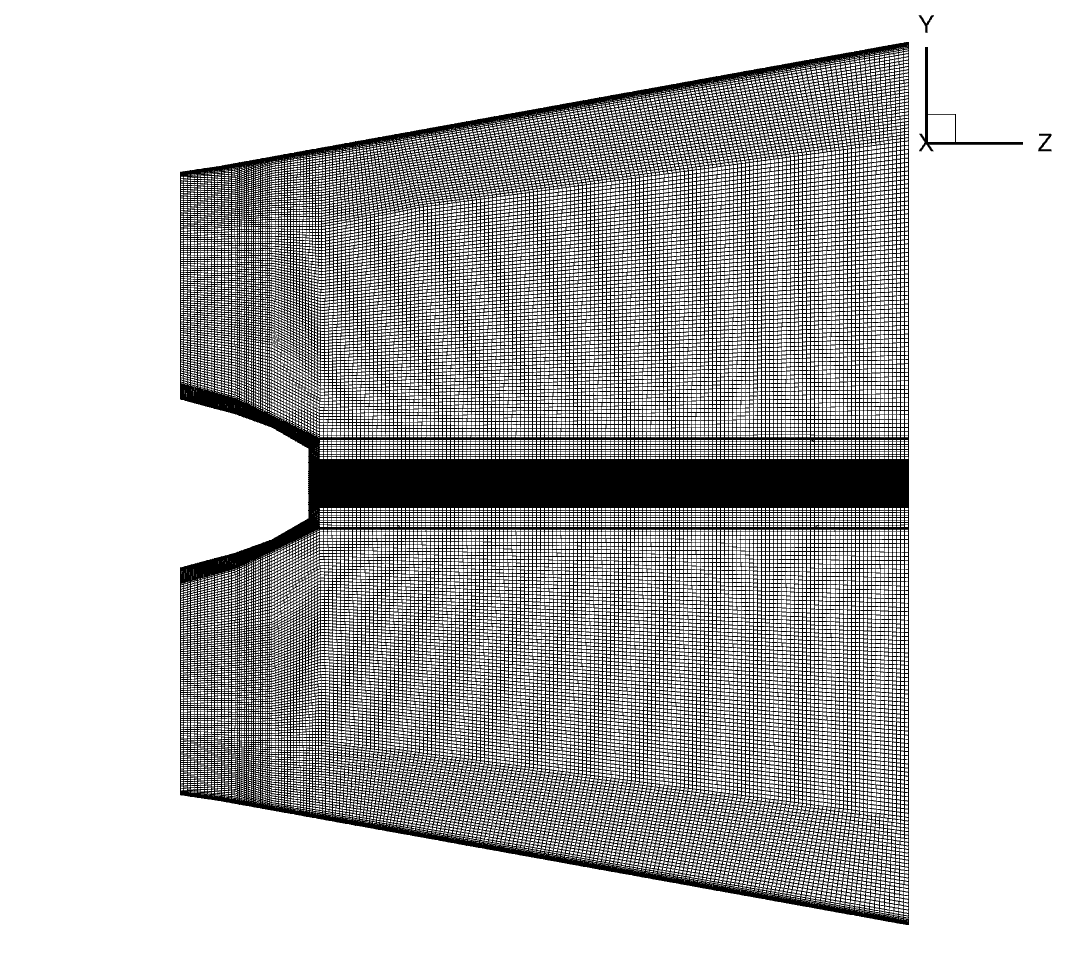
\includegraphics[clip=true, trim= 3.0cm 8.0cm 4.0cm 8.0cm,width=0.325\linewidth]{./figures/bulbt/grid/50m}}       
     \caption{Zoom-in view of the (a)3M (b)14M (c)50M grid. }
     \label{grid2} 
\end{figure*}
%%%%%%%%%%%%%%%%%%%%%%%%%%%%%%%%%%%%%%%%%%%%%%%%%%%%%%%%%%%

No-slip boundary conditions are applied to all solid walls on the rotating hub and the stationary draft tube, while slip boundary conditions are imposed on the solid walls of the extension. The inlet profile is extracted from a numerical simulation conducted with the complete turbine. At the outlet, a zero pressure boundary condition is imposed. The numerical simulations were performed with the baseline MUSCL scheme, the original and extended eddy-preserving limiter scheme. The dissipation of all three schemes were scaled down with a factor of $\alpha=0.375$ in computing the convective flux,
\begin{align} 
\mathbf{F}_{i+\frac{1}{2}} =\frac{1}{2}( \mathbf{F}(\mathbf{W}_{i+\frac{1}{2}}^{L})+\mathbf{F}(\mathbf{W}_{i+\frac{1}{2}}^{R})-\alpha \mathbf{P}^{-1} \lambda (\mathbf{W}_{i+\frac{1}{2}}^{R}-\mathbf{W}_{i+\frac{1}{2}}^{L})),
\label{rusanov}
\end{align}
where $\lambda$ is the spectral radius of the preconditioned Jacobian. The numerical results computed by the three schemes are denoted by ``MUSCL'', ``EDDY'', and ``EDDY-P'' respectively.
%%%%%%%%%%%%%%%%%%%%%%%%%%%%%%%%%%%%%%%%%%%%%%%%%%%%%%%%%%%
%%%%%%%%%%%%%%%%%%%%%%%%%%%%%%%%%%%%%%%%%%%%%%%%%%%%%%%%%%%
%%%%%%%%%%%%%%%%%%%%%%%%%%%%%%%%%%%%%%%%%%%%%%%%%%%%%%%%%%%
%%%%%%%%%%%%%%%%%%%%%%%%%%%%%%%%%%%%%%%%%%%%%%%%%%%%%%%%%%%
%%%%%%%%%%%%%%%%%%%%%%%%%%%%%%%%%%%%%%%%%%%%%%%%%%%%%%%%%%%
%%%%%%%%%%%%%%%%%%%%%%%%%%%%%%%%%%%%%%%%%%%%%%%%%%%%%%%%%%%
%%%%%%%%%%%%%%%%%%%%%%%%%%%%%%%%%%%%%%%%%%%%%%%%%%%%%%%%%%%
%%%%%%%%%%%%%%%%%%%%%%%%%%%%%%%%%%%%%%%%%%%%%%%%%%%%%%%%%%%
%%%%%%%%%%%%%%%%%%%%%%%%%%%%%%%%%%%%%%%%%%%%%%%%%%%%%%%%%%%
\begin{figure}[t]  
\centering      
     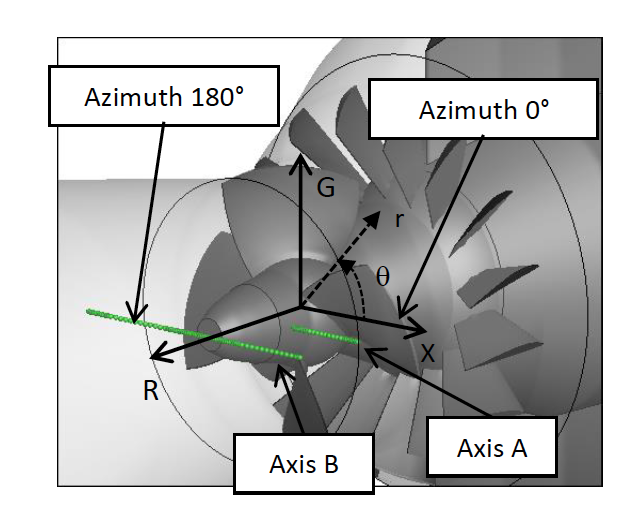
\includegraphics[clip=true, trim= 0.0cm 0.0cm 0.0cm 1.0cm,width=0.99\linewidth]{./figures/bulbt/Location4B}                  
     \caption{Location of 4BY0 \cite{vuillemard2014experimental}.}
     \label{plane4BY0}
\end{figure}
%%%%%%%%%%%%%%%%%%%%%%%%%%%%%%%%%%%%%%%%%%%%%%%%%%%%%%%%%%%
%%%%%%%%%%%%%%%%%%%%%%%%%%%%%%%%%%%%%%%%%%%%%%%%%%%%%%%%%%%
%%%%%%%%%%%%%%%%%%%%%%%%%%%%%%%%%%%
\begin{figure}[t]
\centering
   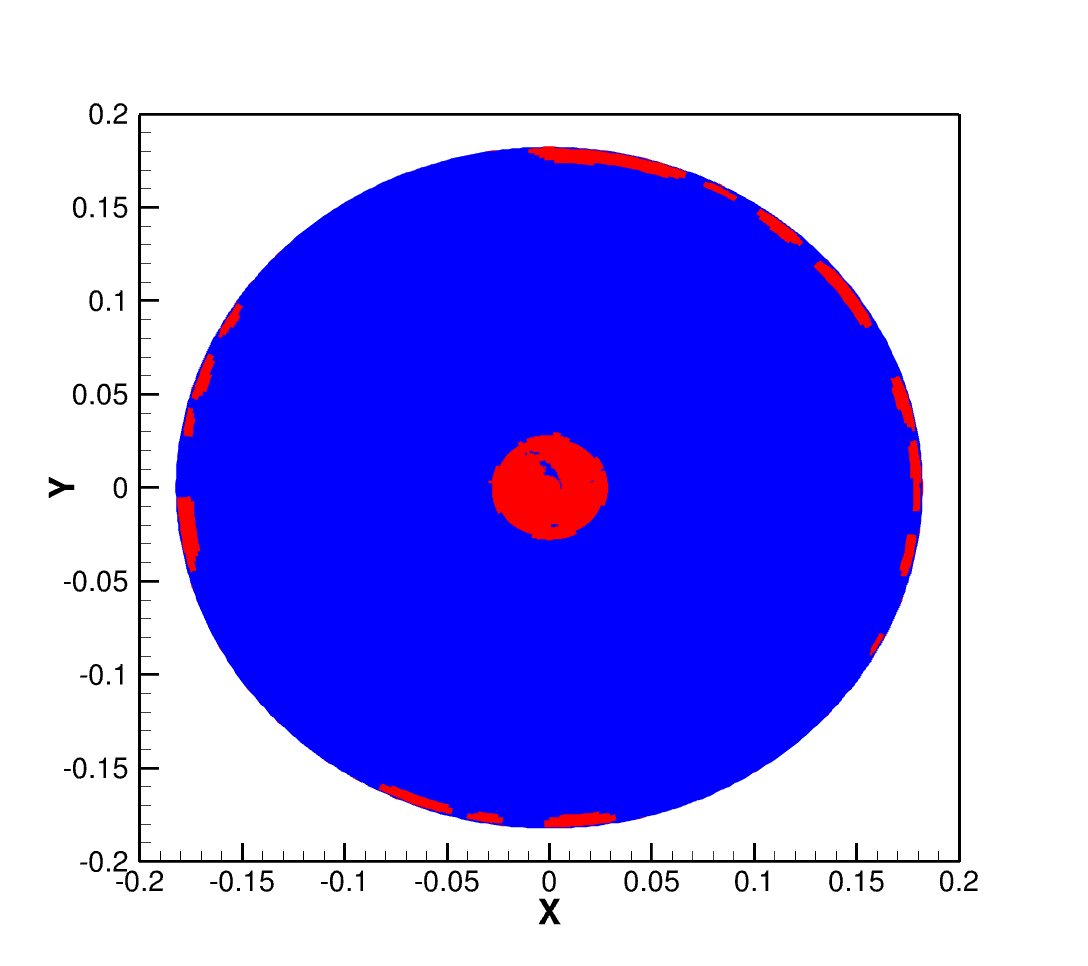
\includegraphics[clip=true, trim= 1.5cm 1.5cm 3.0cm 3.0cm,width=0.99\linewidth]{./figures/bulbt/ivort} 
   \caption{Illustration of regions where the eddy-preserving limiter is active on Plane 4B on the 50M grid.}
   \label{ivort}
\end{figure}
%%%%%%%%%%%%%%%%%%%%%%%%%%%%%%%%%%%
%%%%%%%%%%%%%%%%%%%%%%%%%%%%%%%%%%%%%%%%%%%%%%%%%%%%%%%%%%%
\subsubsection{Velocity Profiles}
In the experiment, the axial and circumferential velocity profiles were measured by the Laser Doppler Velocimetry (LDV) along $y=0$ of Plane 4B, which is the green line labeled as Axis B in Fig.~\ref{plane4BY0}. This location is referred as 4BY0.

Velocity profiles are normalized with the reference velocity $U_{ref}$, which is calculated by,
\begin{align} 
   U_{ref} = \frac{Q_{dis}}{\pi (\frac{1}{2}D_{ref})^2},
\end{align}
where $Q_{dis}$ is the volumetric flow rate at corresponding OPs.
As shown in Fig.~\ref{w} and Fig.~\ref{v}, the global trends of the experimental axial and circumferential velocities are captured, and on each grid, the velocity profiles computed by all schemes are almost identical. However, zoom-in views of the velocity profiles show some discrepancies in the central region. 

In the zoom-in view of the axial velocity profile in Fig.~\ref{zw}, the experimental data shows a backflow downstream of the hub \cite{vuillemard2014experimental}. The MUSCL scheme shows poor predictions of the backflow region on all three grids. Although EDDY and EDDY-P schemes predict similar profiles to the MUSCL scheme on the 3M grid, they are able to resolve the backflow region on the 14M and 50M grids, and the predictions improve towards the experimental data as the grid was refined. A marked difference is noted on the 14M grid, where the trend towards an increasing axial velocity in the upstream direction until the centerline is reported in both the experimental data as well as the EDDY and EDDY-P schemes. It will be shown in the subsequent section that this is primarily due to the lower artificial dissipation within this region. Furthermore, the backflow predicted by the EDDY-P scheme is slightly closer to the experimental data than the EDDY scheme.

As for the experimental circumferential velocity, three zones are clearly identified: an inner co-rotating zone downstream of the hub; an outer co-rotating zone from the cone wall; and a counter-rotating zone in-between \cite{vuillemard2014experimental}. The circumferential velocity first accelerates from the centre point in the direction of the runner rotation gently to a local maximum, which represents a forced vortex induced by the rotating hub. It then decelerates to zero, where the flow rotational direction is reversed, and the inner co-rotating zone is formed from the centre point to this position. The circumferential velocity then subsequently accelerates in the reversed direction to a local maximum and then decelerates. It continues to decelerate to zero and forms the counter-rotating zone.  A shear flow is formed by the inner co-rotating zone and the counter-rotating zone at approximately $r/D_{ref}=\pm 0.068$. The flow then changes to a co-rotating direction until it reaches the cone wall. The zoom-in view in Fig.~\ref{zv} shows the circumferential velocity in the inner co-rotating zone and the counter-rotating zone. All schemes do not predict the circumferential velocity very well in the central region on the 3M grid. On the 14M and 50M grids, although the MUSCL scheme has improved slightly, it still behaves poorly from the centre point to the position of maximum velocity in the counter-rotating zone; in comparison, the EDDY and EDDY-P schemes predict better the location of the maximum velocity and the low and constant circumferential velocity within the inner co-rotating zone. Similar to that observed in the axis velocity distribution, both EDDY and EDDY-P begin to show the correct trends by the 14M grid.

Figure~\ref{w1} and Figure~\ref{w2} show the contours of axial velocity and two dimensional streamlines at plane $y=0$ on 14M and 50M grids. The axial velocity decelerates rapidly from the inlet to the end of the hub, as the cross section expands drastically. Flow separation takes place on the wall of the hub and a backflow region is formed downstream of the hub. Comparing the results of the MUSCL scheme against the EDDY and EDDY-P schemes, it can be clearly seen that the EDDY and EDDY-P schemes predict a wider and longer backflow region fully attached to the hub. After the hub, the flows merge into one and continue to decelerate, but at a slower rate.

There are several challenges for numerical schemes in predicting the velocity profiles at 4BY0. For the axial velocity, it has a local minimum and a backflow region, while for the circumferential velocity, there are two co-rotating and one counter-rotating zone. The velocity components are constrained by the divergence free condition for incompressible flows. Furthermore, the adverse pressure gradient needs to be accurately resolved to ensure that the flow decelerates appropriately, and the flow separation takes place at the correct location. Tackling these challenges requires highly accurate numerical schemes, and the comparisons illustrate that the MUSCL scheme generally fails to predicting these features, while the developed low dissipative EDDY and EDDY-P schemes have outperformed significantly over the MUSCL scheme. As shown in Fig.~\ref{ivort}, the contours in red represent vortical regions detected on Plane 4B on the 50M grid. The central core region has a radius of approximately 0.03, which not only covers the entire inner co-rotating zone, but also the shear flows formed by the inner co-rotating zone and the counter-rotating zone. On these regions, the eddy-preserving limiter is active; the velocity components are transferred into the vortical system, and the van Albada limiters on the swirl plane are switched off to reduce the dissipation for preserving the vortical motions. As a consequence, the EDDY and EDDY-P schemes are able to better resolve the inner co-rotating zone and the shear flows as demonstrated in Fig.~\ref{zv}.
%%%%%%%%%%%%%%%%%%%%%%%%%%%%%%%%%%%%%%%%%%%%%%%%%%%%%%%%%%%
%%%%%%%%%%%%%%%%%%%%%%%%%%%%%%%%%%%%%%%%%%%%%%%%%%%%%%%%%%%
%%%%%%%%%%%%%%%%%%%%%%%%%%%%%%%%%%%%%%%%%%%%%%%%%%%%%%%%%%%
\subsubsection{Turbulent Kinetic Energy Profiles}
The results for the turbulent kinetic energy (TKE)  at 4BY0 are plotted in Fig.~\ref{tke}. There are several peaks found in the experimental profile. Two higher peaks at approximately $r/D_{ref}=\pm 0.068$ corresponds to the shear flows formed by the inner co-rotating zone and the counter-rotating zone. Two lower peaks corresponds to the shear layer near the cone walls. Overall, the TKE profiles were underpredicted by all schemes in most of the region. In the zoom-in view of Fig.~\ref{ztke}, incorrect TKE peaks appear in the central region, which are mainly due to the large gradients of the computed velocity profiles in Fig.~\ref{zv}. As the grid was refined, the predictions of flows downstream of the hub have improved, leading to a reduction of the incorrect TKE peak at the central core; while the shear flow has been better formed between the inner co-rotating zone and the counter-rotating zone, the two side peaks edge upwards, showing a clear improvement towards the experimental data. On each grid, compared to the MUSCL scheme, the EDDY and EDDY-P schemes predict slightly higher values at the two side peaks and lower values in the central core region, which leads to better agreement against the experimental data. 
%%%%%%%%%%%%%%%%%%%%%%%%%%%%%%%%%%%%%%%%%%%%%%%%%%%%%%%%%%%
%%%%%%%%%%%%%%%%%%%%%%%%%%%%%%%%%%%%%%%%%%%%%%%%%%%%%%%%%%%
%%%%%%%%%%%%%%%%%%%%%%%%%%%%%%%%%%%%%%%%%%%%%%%%%%%%%%%%%%%
\subsubsection{Vorticity Magnitude Profiles}
The profiles of the vorticity magnitude in the central region of 4BY0 are plotted in Fig.~\ref{vo}. Due to lack of an experimental radial velocity profile, the experimental vorticity magnitude was computed with the assumption that the flow is uniform in the circumferential direction. This is certainly not what would be observed in the experimental data; however, this assumption is sufficient for the purpose of comparing numerical schemes. 

Three peaks are shown in the experimental profile. The central peak represents the forced vortex induced by the rotating hub, while the two side peaks at approximately $r/D_{ref}=\pm 0.068$ represent the shear flows formed by the inner co-rotating zone and the counter-rotating zone. Since OP2 is close to the BEP, the draft tube flow is expected to have very weak swirls. This can be seen from the experimental data in Fig.~\ref{zv}, where the circumferential profiles near the centre point have very gentle slopes. On the 3M grid, all schemes overpredict the vorticity magnitude in the centre, due to the mispredicted gradients of the circumferential velocity, as shown in Fig.~\ref{zv}(a). The overprediction of the vorticity in the central region partially contributes to the overproduction of the TKE in Fig.~\ref{ztke}, which will result in excessive dissipation, and deteriorate the predictions of velocity profiles downstream of the hub. On the 14M and 50M grids, the MUSCL scheme still overpredicts the peak in the centre, while the EDDY and EDDY-P schemes only slightly underpredicts the peak. It is also notable that as the grid was refined, the two side peaks due to the shear flows were captured mildly by the MUSCL scheme and very well by the EDDY schemes on the 14M; while all three schemes resolved the peaks on the 50M grid. 

%%%%%%%%%%%%%%%%%%%%%%%%%%%%%%%%%%%%%%%%%%%%%%%%%%%%%%%%%%%
%%%%%%%%%%%%%%%%%%%%%%%%%%%%%%%%%%%%%%%%%%%%%%%%%%%%%%%%%%%
%%%%%%%%%%%%%%%%%%%%%%%%%%%%%%%%%%%%%%%%%%%%%%%%%%%%%%%%%%%
\subsubsection{Pressure Profiles}
The pressure profiles at 4BY0 are compared in Fig.~\ref{p}. The numerical result computed by the EDDY-P scheme on the 50M grid is employed as a reference, due to the lack of an experimental distribution of pressure across the cross-section of the draft tube, and denoted by ``EDDY-P-50M''. The EDDY-P scheme was used as the reference for two reasons; first, as the grid is refined, all schemes tend towards the results of the EDDY-P scheme on the 50M grid; and second, the EDDY-P pressure distribution seems more invariant to the grid refinement. The relative $L^{2}$ norms of difference against ``EDDY-P-50M'' for all schemes on all grids are shown in Tab.~\ref{table2}. 

Since the swirl flow is weak in the central region in the experiment, according to the steady incompressible momentum equations, the gradient of the pressure is also expected to be small. However, on the 3M grid, all three schemes produce large incorrect peaks in the pressure profile. This is due to the mispredicted gradients of the circumferential velocity near the central region in Fig.~\ref{zv}(a). It can be explained alternatively by the overprediction of the vorticity magnitude in Fig.~\ref{vo}(a), since the minimum pressure is usually lower in a stronger forced vortex. On the 14M grid, the incorrect peaks of EDDY and EDDY-P are almost removed, and the prediction by the MUSCL scheme has improved. Moreover, compared to the prediction by EDDY, the prediction of EDDY-P is closer to the reference profile EDDY-P-50M, which demonstrates that the dissipation of the scheme is further reduced. On the 50M grid, the peak for MUSCL continues to diminish, and the predictions of EDDY and EDDY-P are almost equivalent. In summary, the EDDY and EDDY-P schemes produced better pressure profiles than the MUSCL scheme, and the EDDY-P is less dissipative than EDDY as expected. 
%%%%%%%%%%%%%%%%%%%%%%%%%%%%%%%%%%%%%%%%%%%%%%%%%%%%%%%%%%%
%%%%%%%%%%%%%%%%%%%%%%%%%%%%%%%%%%%%%%%%%%%%%%%%%%%%%%%%%%%
%%%%%%%%%%%%%%%%%%%%%%%%%%%%%%%%%%%%%%%%%%%%%%%%%%%%%%%%%%%
%%%%%%%%%%%%%%%%%%%%%%%%%%%%%%%%%%%%%%%%%%%%%%%%%%%%%%%%%%%
%%%%%%%%%%%%%%%%%%%%%%%%%%%%%%%%%%%%%%%%%%%%%%%%%%%%%%%%%%%
%%%%%%%%%%%%%%%%%%%%%%%%%%%%%%%%%%%%%%%%%%%%%%%%%%%%%%%%%%%
\subsubsection{Recovery Coefficient}
The recovery coefficient is selected as a global quantity for evaluating the overall performance of the draft tube in converting dynamic pressure into static pressure. A generalized definition of the recovery coefficient is given by \cite{fox1971effects}: 
\begin{align} 
\chi&=\frac{p_{outlet}-p_{inlet}}{q}\\
&=\frac{\frac{\rho}{\dot{m}}\underset{S_{outlet}}{\int}p\mathbf{v}\cdot \vec{n}dS-\frac{\rho}{\dot{m}}\underset{S_{inlet}}{\int}p\mathbf{v}\cdot \vec{n}dS}{\frac{1}{2S_{inlet}}\rho\underset{S_{inlet}}{\int}\mathbf{v}\cdot\mathbf{v}dS}, 
\end{align}
where $q$, $\dot{m}$ and $S$ are the dynamic pressure, mass flow rate, and cross-sectional area respectively. The recovery coefficients from the inlet to the outlet are given in Tab.~\ref{rc}. It is observed that the computed recovery coefficients are generally higher on coarser grids. On the 14M and 50M grids, recovery coefficients computed by all three schemes are quite close to each other. This reveals that for OPs near the BEP, where strong pressure fluctuation does not exist, the MUSCL scheme is able to provide similar prediction on the overall recovery coefficients compared to the less dissipative schemes EDDY and EDDY-P on moderately fine grids, even if the MUSCL scheme fails in predicting some regional velocity profiles.
%%%%%%%%%%%%%%%%%%%%%%%%%%%%%%%%%%%%%%%%%%%%%%%%%%%%%%%%%%%%%%%%
%%%%%%%%%%%%%%%%%%%%%%%%%%%%%%%%%%%%%%%%%%%%%%%%%%%%%%%%%%%%%%%%
%%%%%%%%%%%%%%%%%%%%%%%%%%%%%%%%%%%%%%%%%%%%%%%%%%%%%%%%%%%%%%%%
%%%%%%%%%%%%%%%%%%%%%%%%%%%%%%%%%%%%%%%%%%%%%%%%%%%%%%%%%%%%%%%%
%%%%%%%%%%%%%%%%%%%%%%%%%%%%%%%%%%%%%%%%%%%%%%%%%%%%%%%%%%%%%%%%
\begin{figure}[t]  
\centering
     \subfigure[]{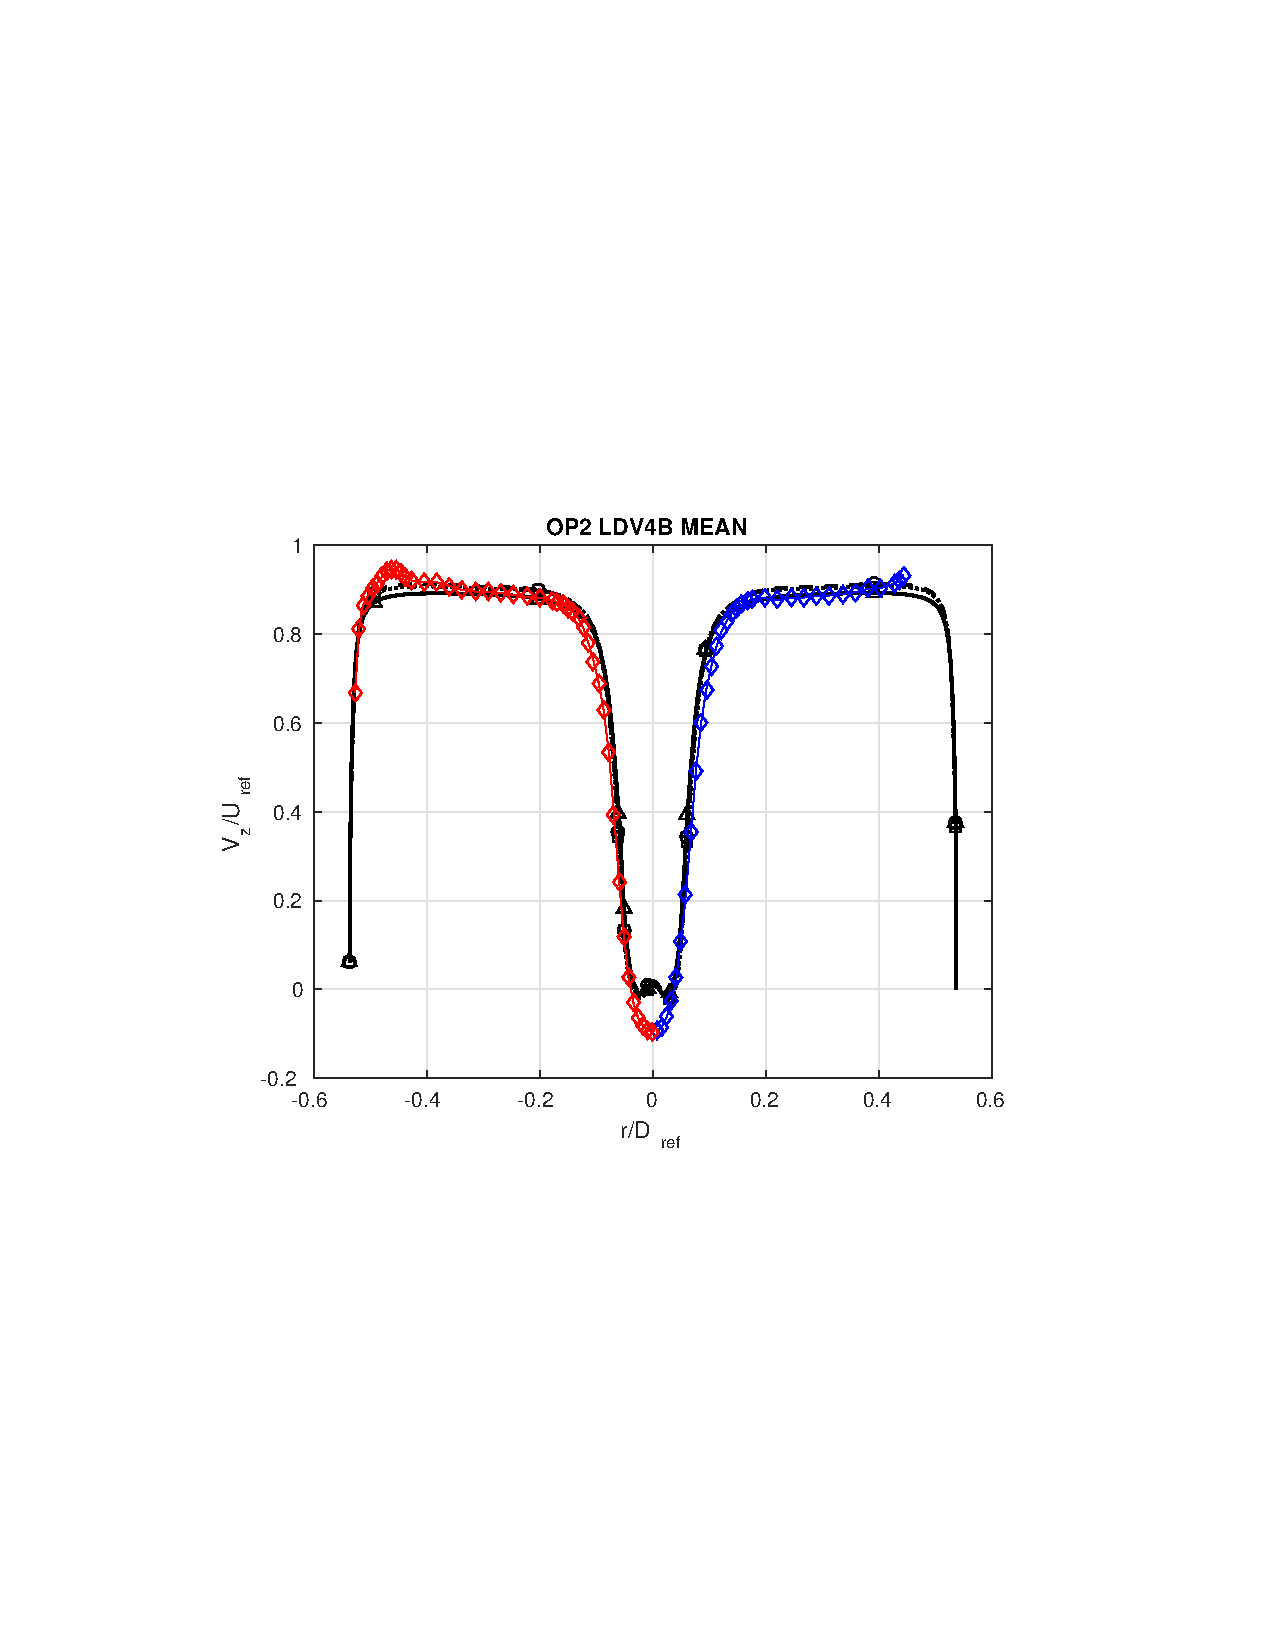
\includegraphics[clip=true, trim= 3.0cm 8.0cm 4.0cm 8.0cm,width=0.98\linewidth]{./figures/bulbt/4BY0/3m/multi_plan4BY0_BulbT_op2_uncert_X_w}} \\             
     \subfigure[]{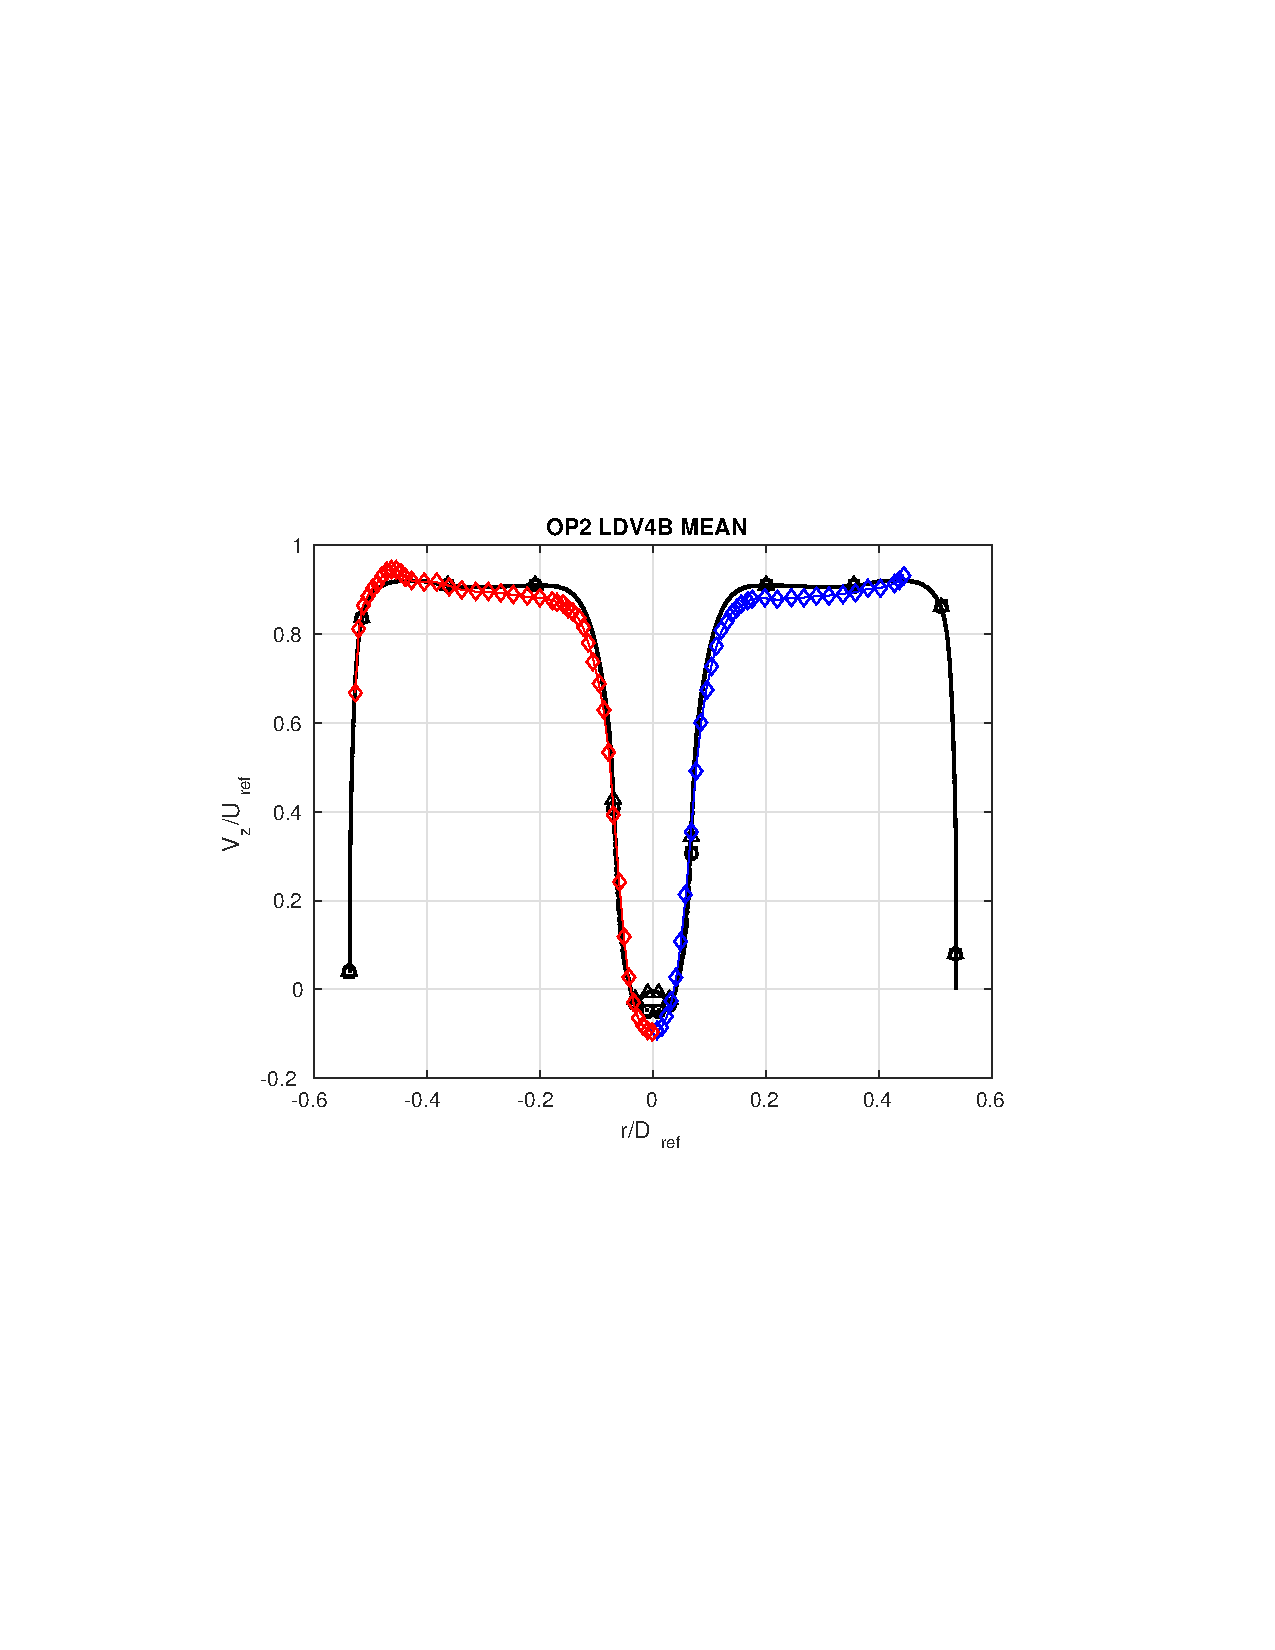
\includegraphics[clip=true, trim= 3.0cm 8.0cm 4.0cm 8.0cm,width=0.98\linewidth]{./figures/bulbt/4BY0/14m/multi_plan4BY0_BulbT_op2_uncert_X_w}} \\
     \subfigure[]{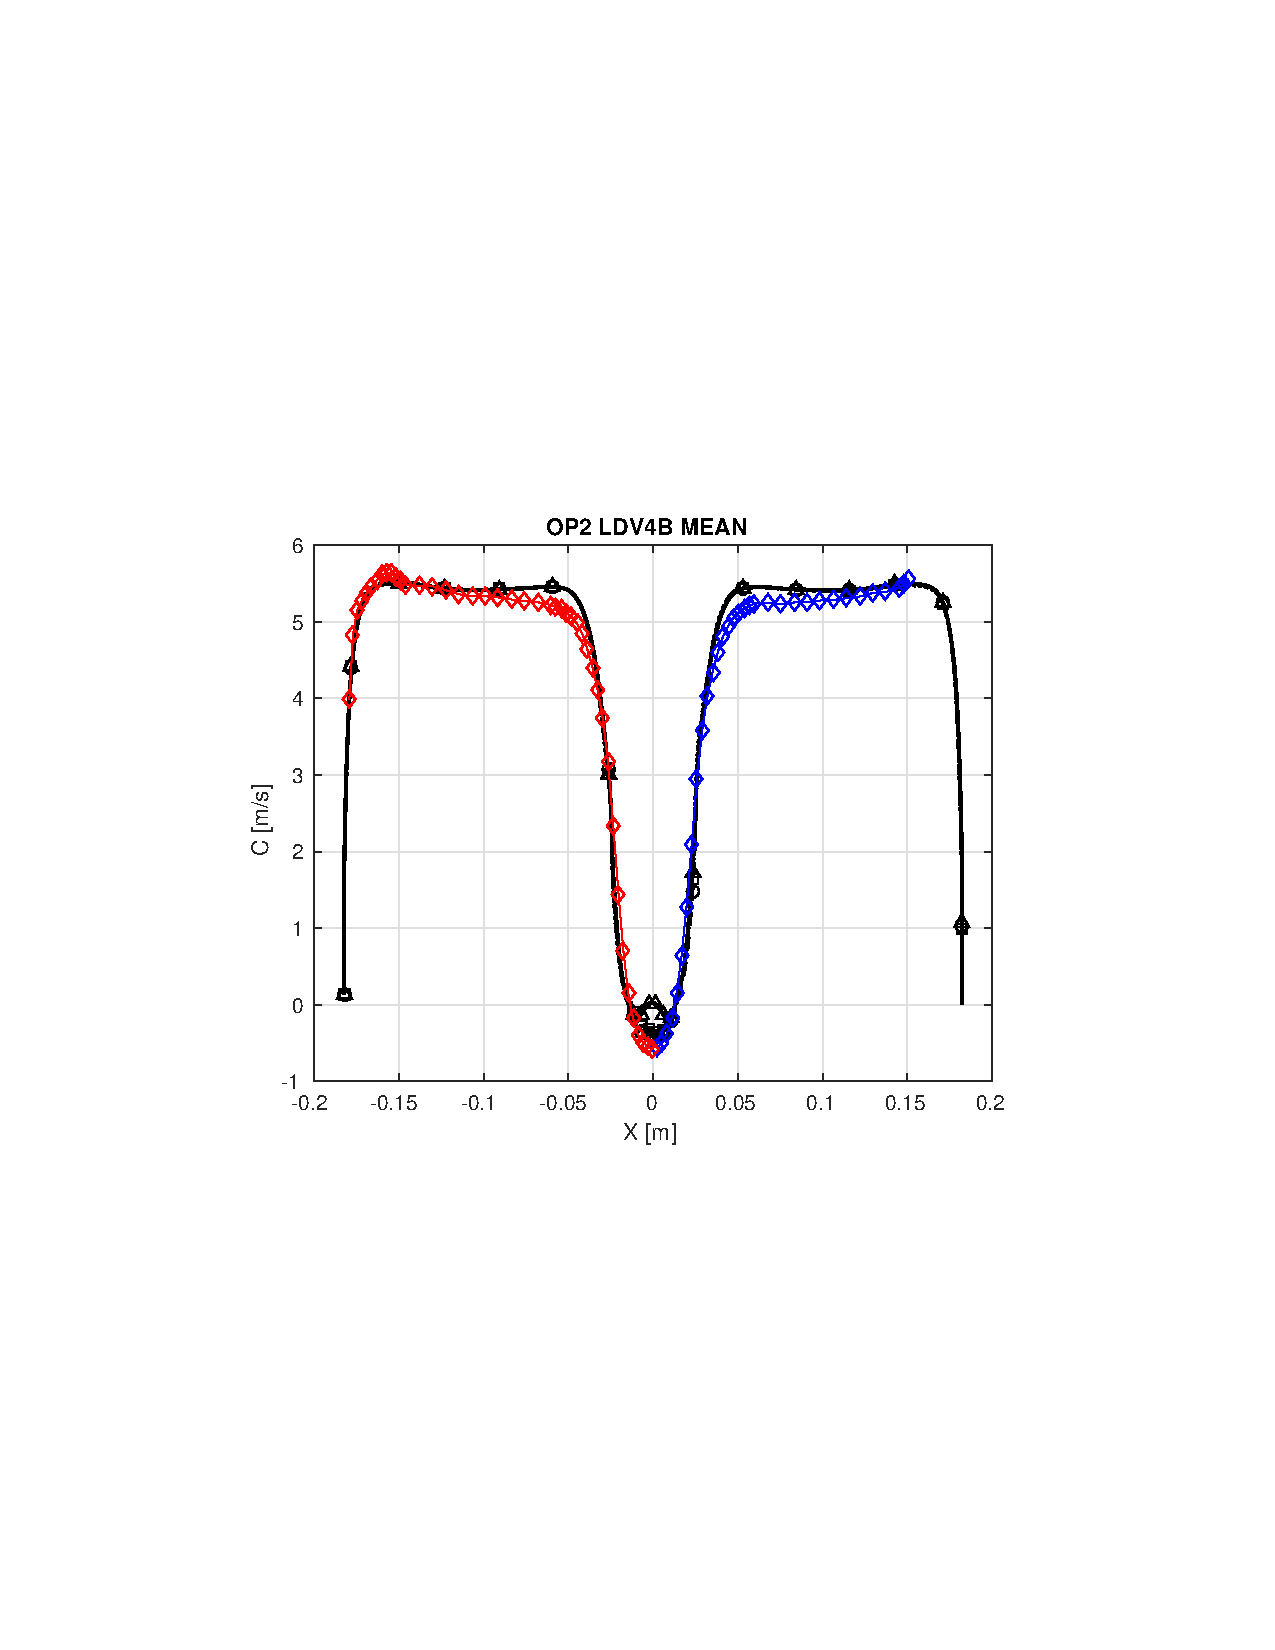
\includegraphics[clip=true, trim= 3.0cm 8.0cm 4.0cm 8.0cm,width=0.98\linewidth]{./figures/bulbt/4BY0/50m/multi_plan4BY0_BulbT_op2_uncert_X_w}}       
     \caption{Axial velocity profiles at 4BY0 on (a)3M (b)14M (c)50M grid. (MUSCL: \mline; EDDY: \eline; EDDY-P: \epline; EXP Az0: \bluediam; EXP Az180: \reddiam.)}
     \label{w}      
\end{figure}
%%%%%%%%%%%%%%%%%%%%%%%%%%%%%%%%%%%%%%%%%%%%%%%%%%%%%%%%%%%%%%%%
\begin{figure}[t]  
\centering
     \subfigure[]{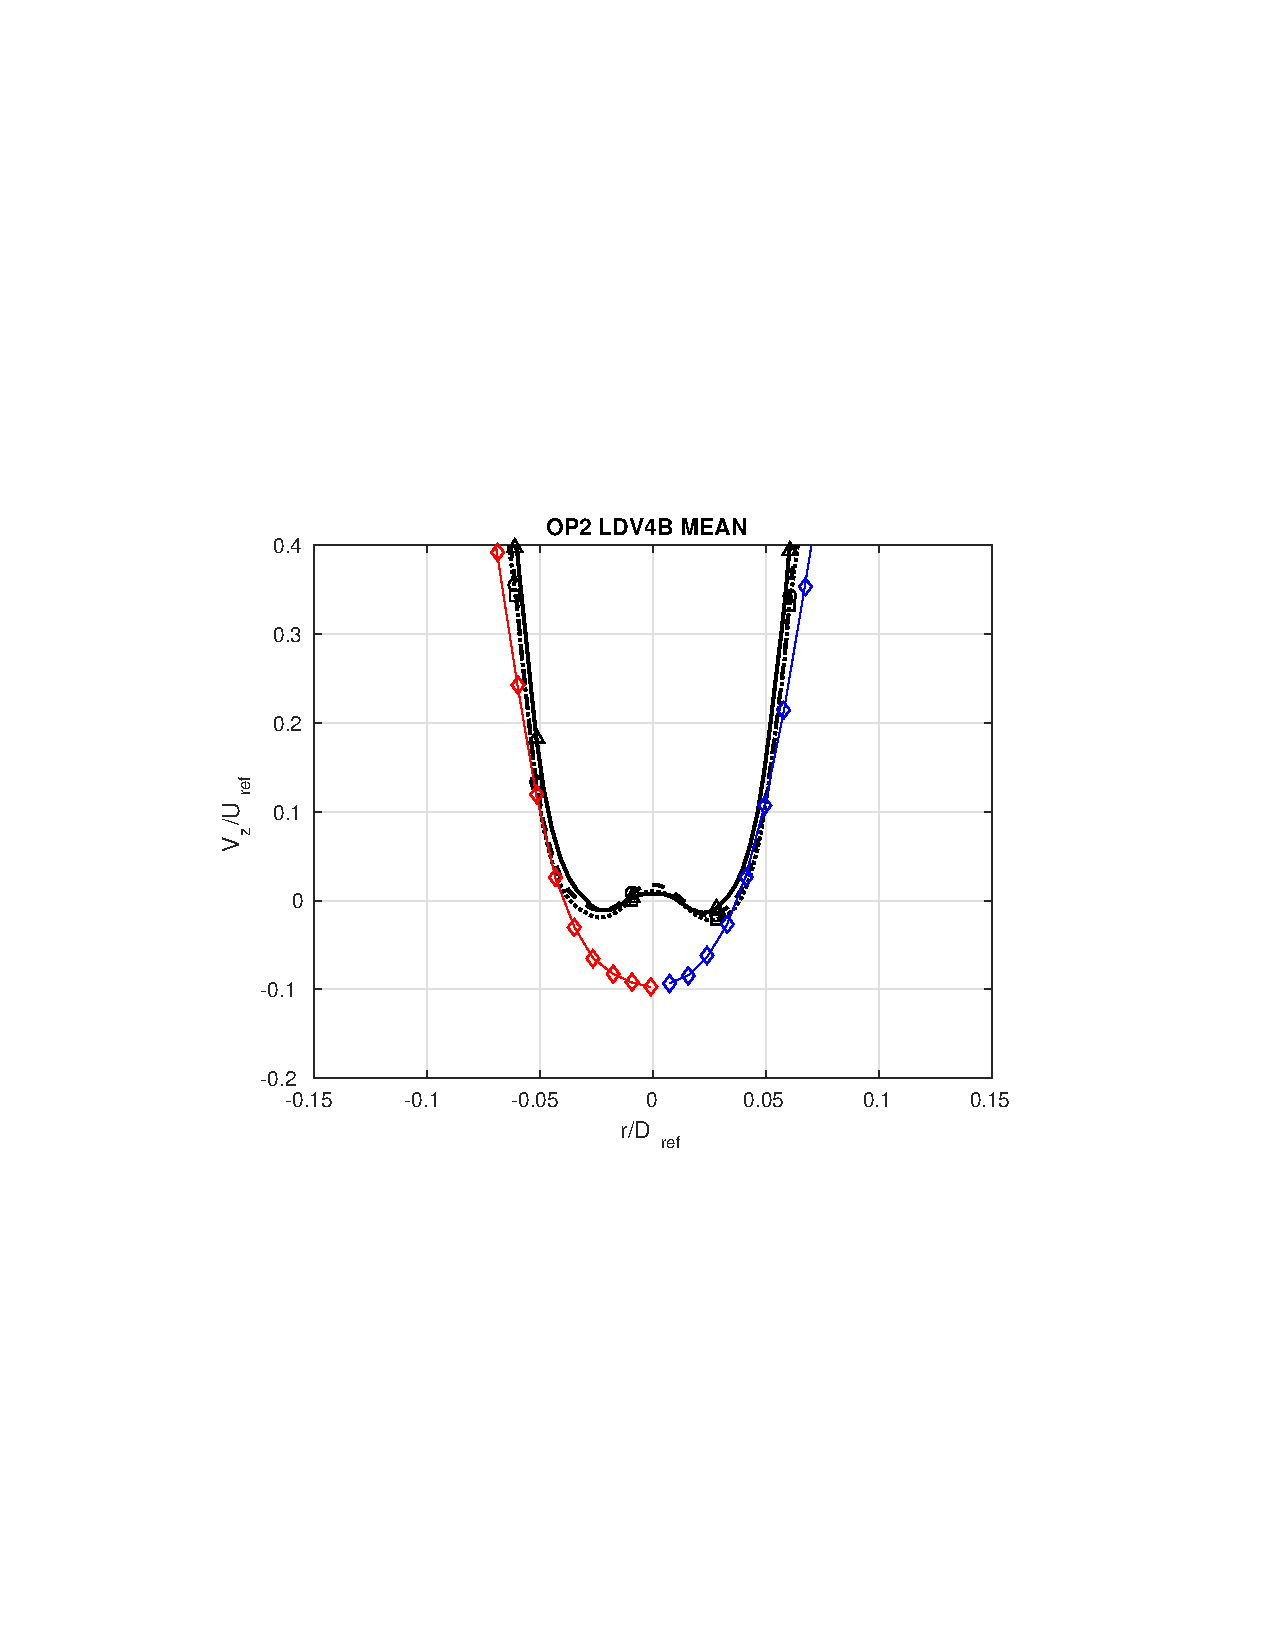
\includegraphics[clip=true, trim= 3.0cm 8.0cm 4.0cm 8.0cm,width=0.98\linewidth]{./figures/bulbt/4BY0/3m/zoom_multi_plan4BY0_BulbT_op2_uncert_X_w}} \\             
     \subfigure[]{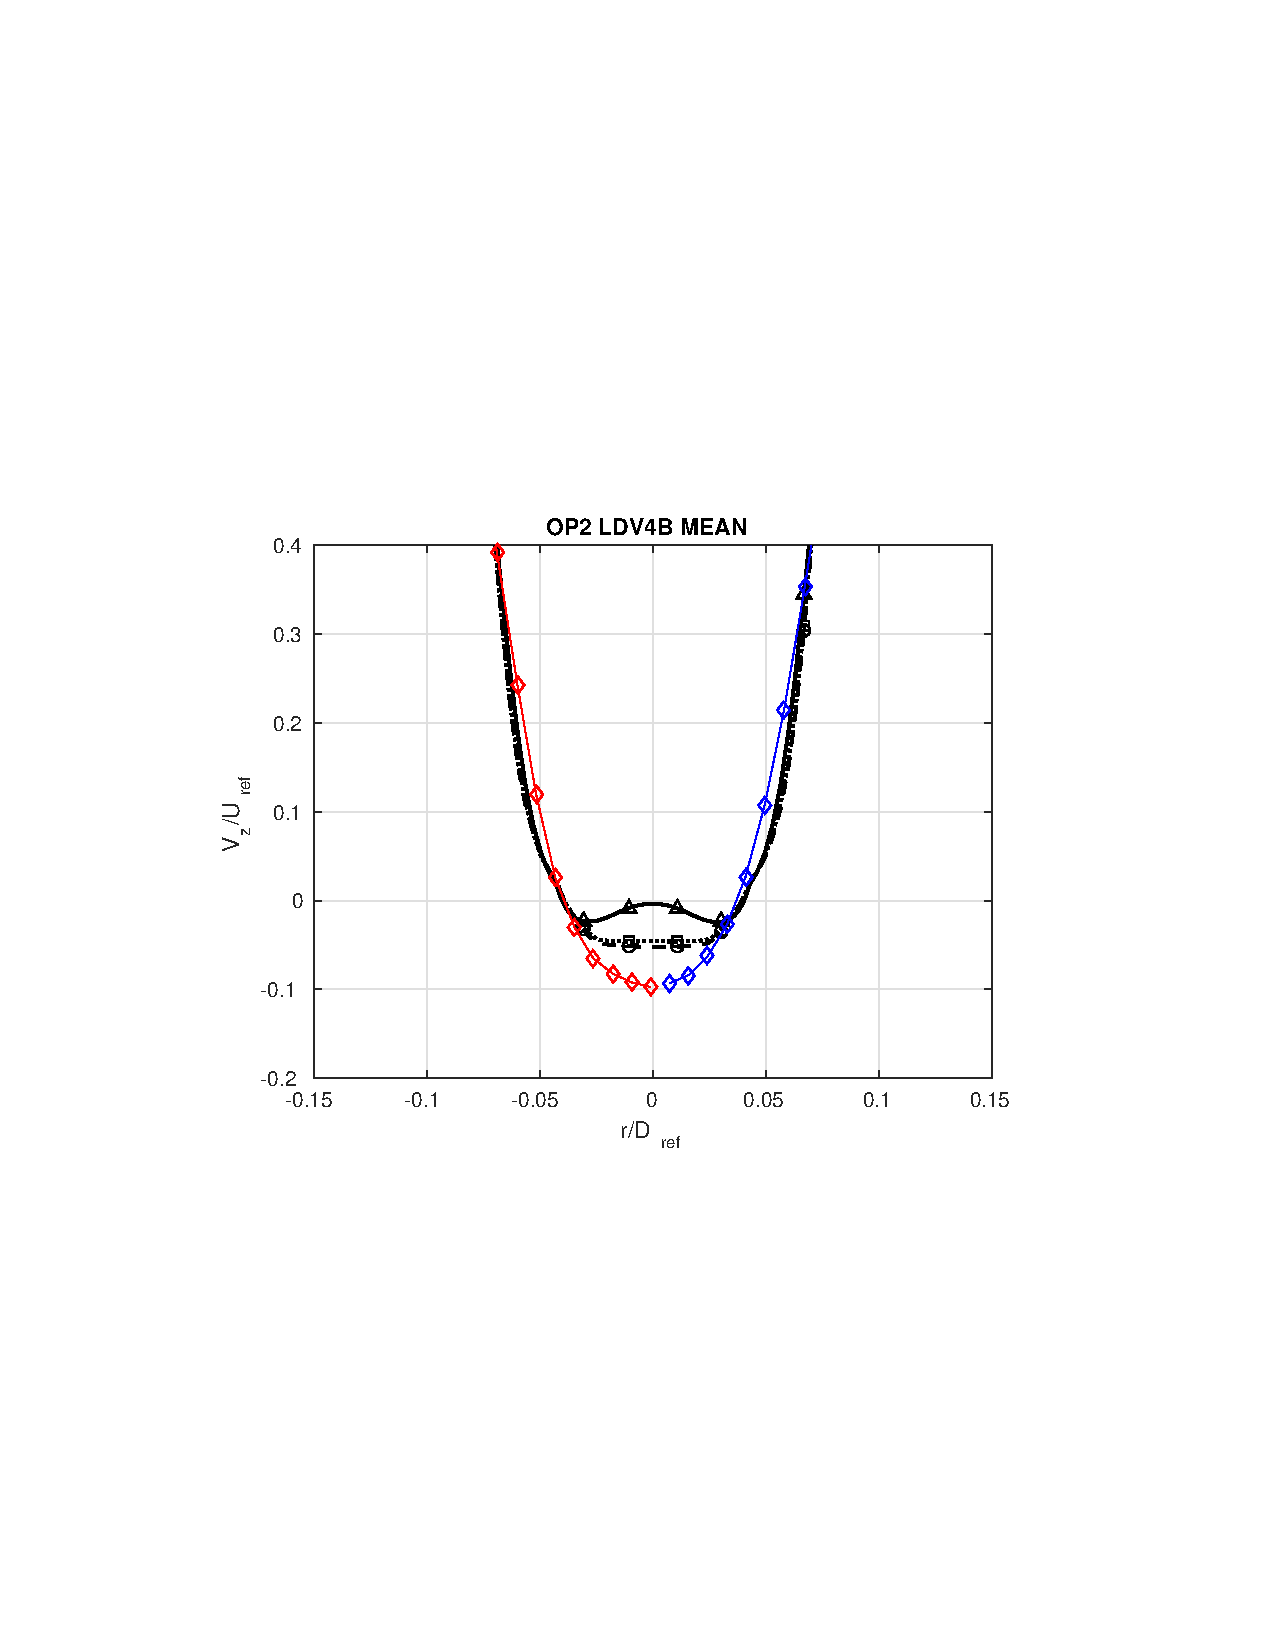
\includegraphics[clip=true, trim= 3.0cm 8.0cm 4.0cm 8.0cm,width=0.98\linewidth]{./figures/bulbt/4BY0/14m/zoom_multi_plan4BY0_BulbT_op2_uncert_X_w}} \\
     \subfigure[]{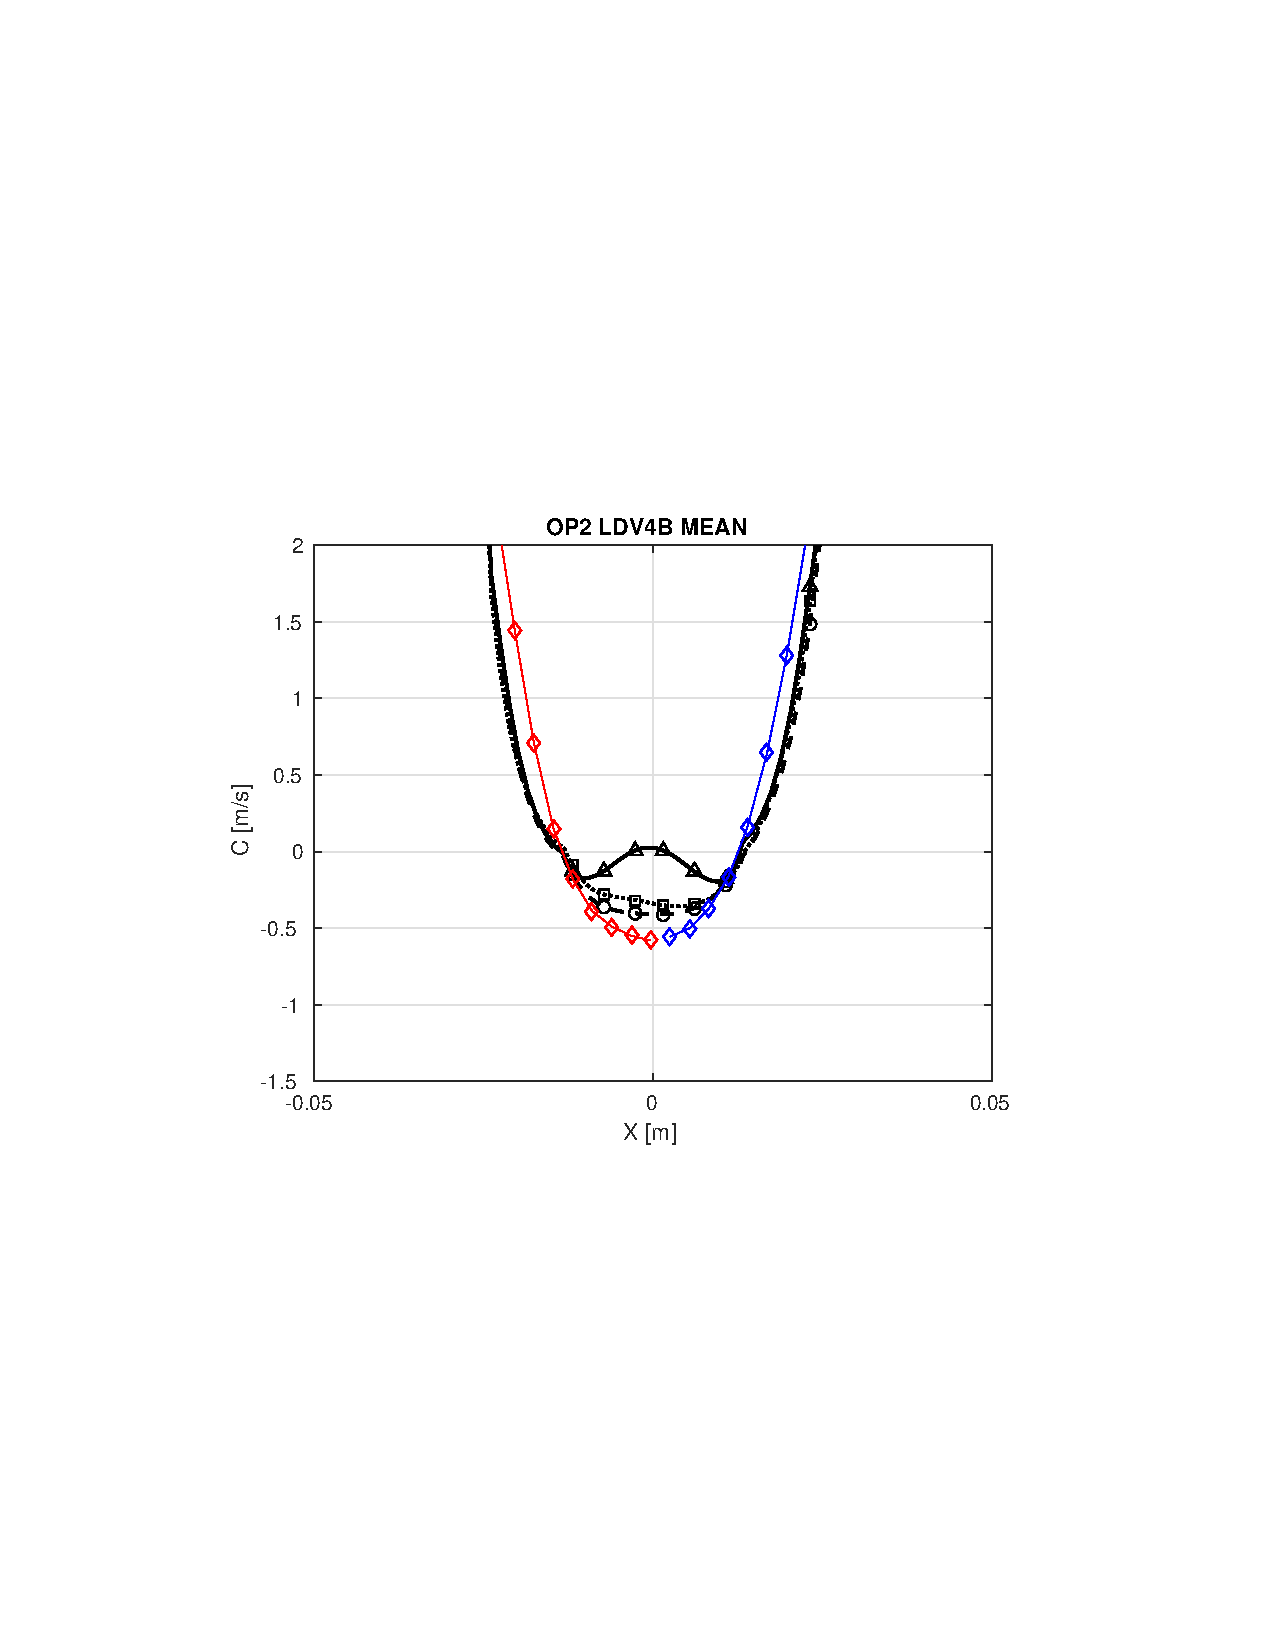
\includegraphics[clip=true, trim= 3.0cm 8.0cm 4.0cm 8.0cm,width=0.98\linewidth]{./figures/bulbt/4BY0/50m/zoom_multi_plan4BY0_BulbT_op2_uncert_X_w}}     
     \caption{Zoom-in view of axial velocity profiles at 4BY0 on (a)3M (b)14M (c)50M grid. (MUSCL: \mline; EDDY: \eline; EDDY-P: \epline; EXP Az0: \bluediam; EXP Az180: \reddiam.)}
     \label{zw}       
\end{figure}
%%%%%%%%%%%%%%%%%%%%%%%%%%%%%%%%%%%%%%%%%%%%%%%%%%%%%%%%%%%%%%%%
%%%%%%%%%%%%%%%%%%%%%%%%%%%%%%%%%%%%%%%%%%%%%%%%%%%%%%%%%%%%%%%%
\begin{figure}[t]  
\centering
     \subfigure[]{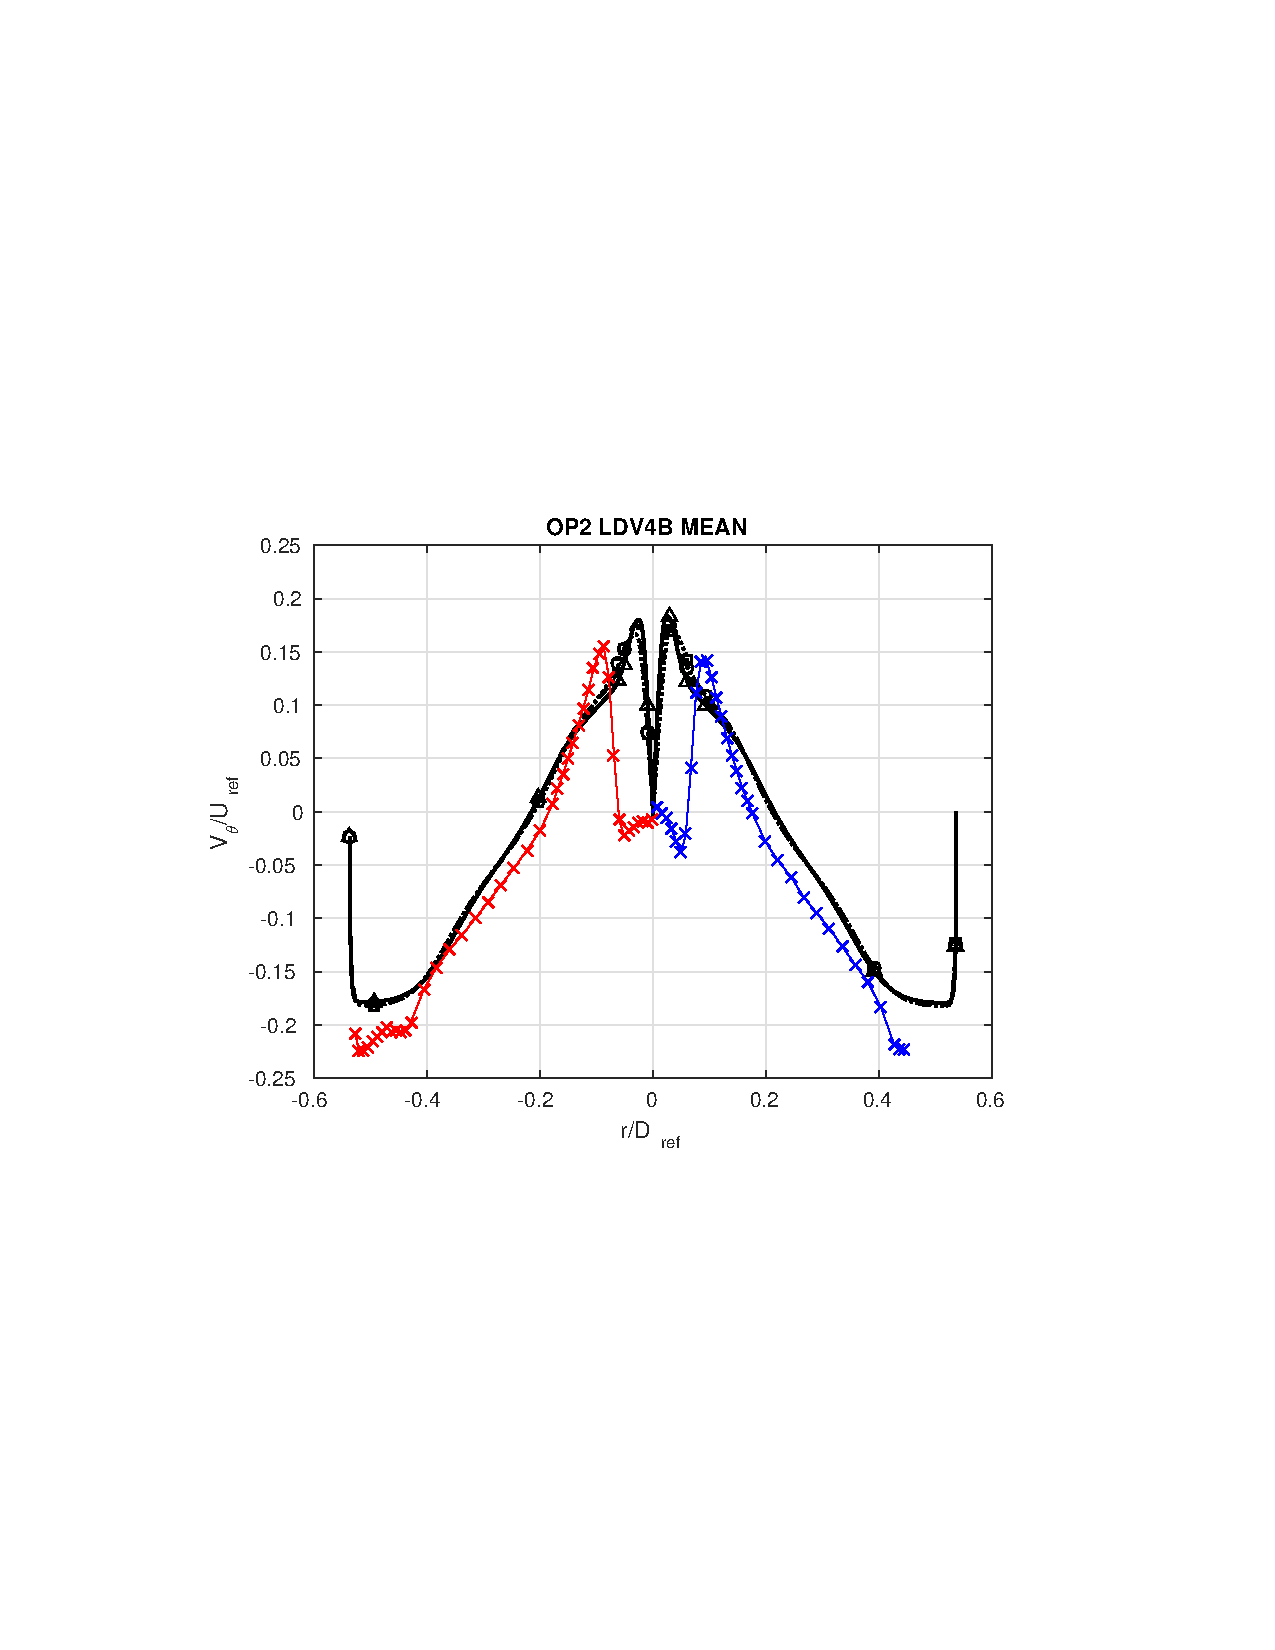
\includegraphics[clip=true, trim= 3.0cm 8.0cm 4.0cm 8.0cm,width=0.98\linewidth]{./figures/bulbt/4BY0/3m/multi_plan4BY0_BulbT_op2_uncert_X_v}} \\             
     \subfigure[]{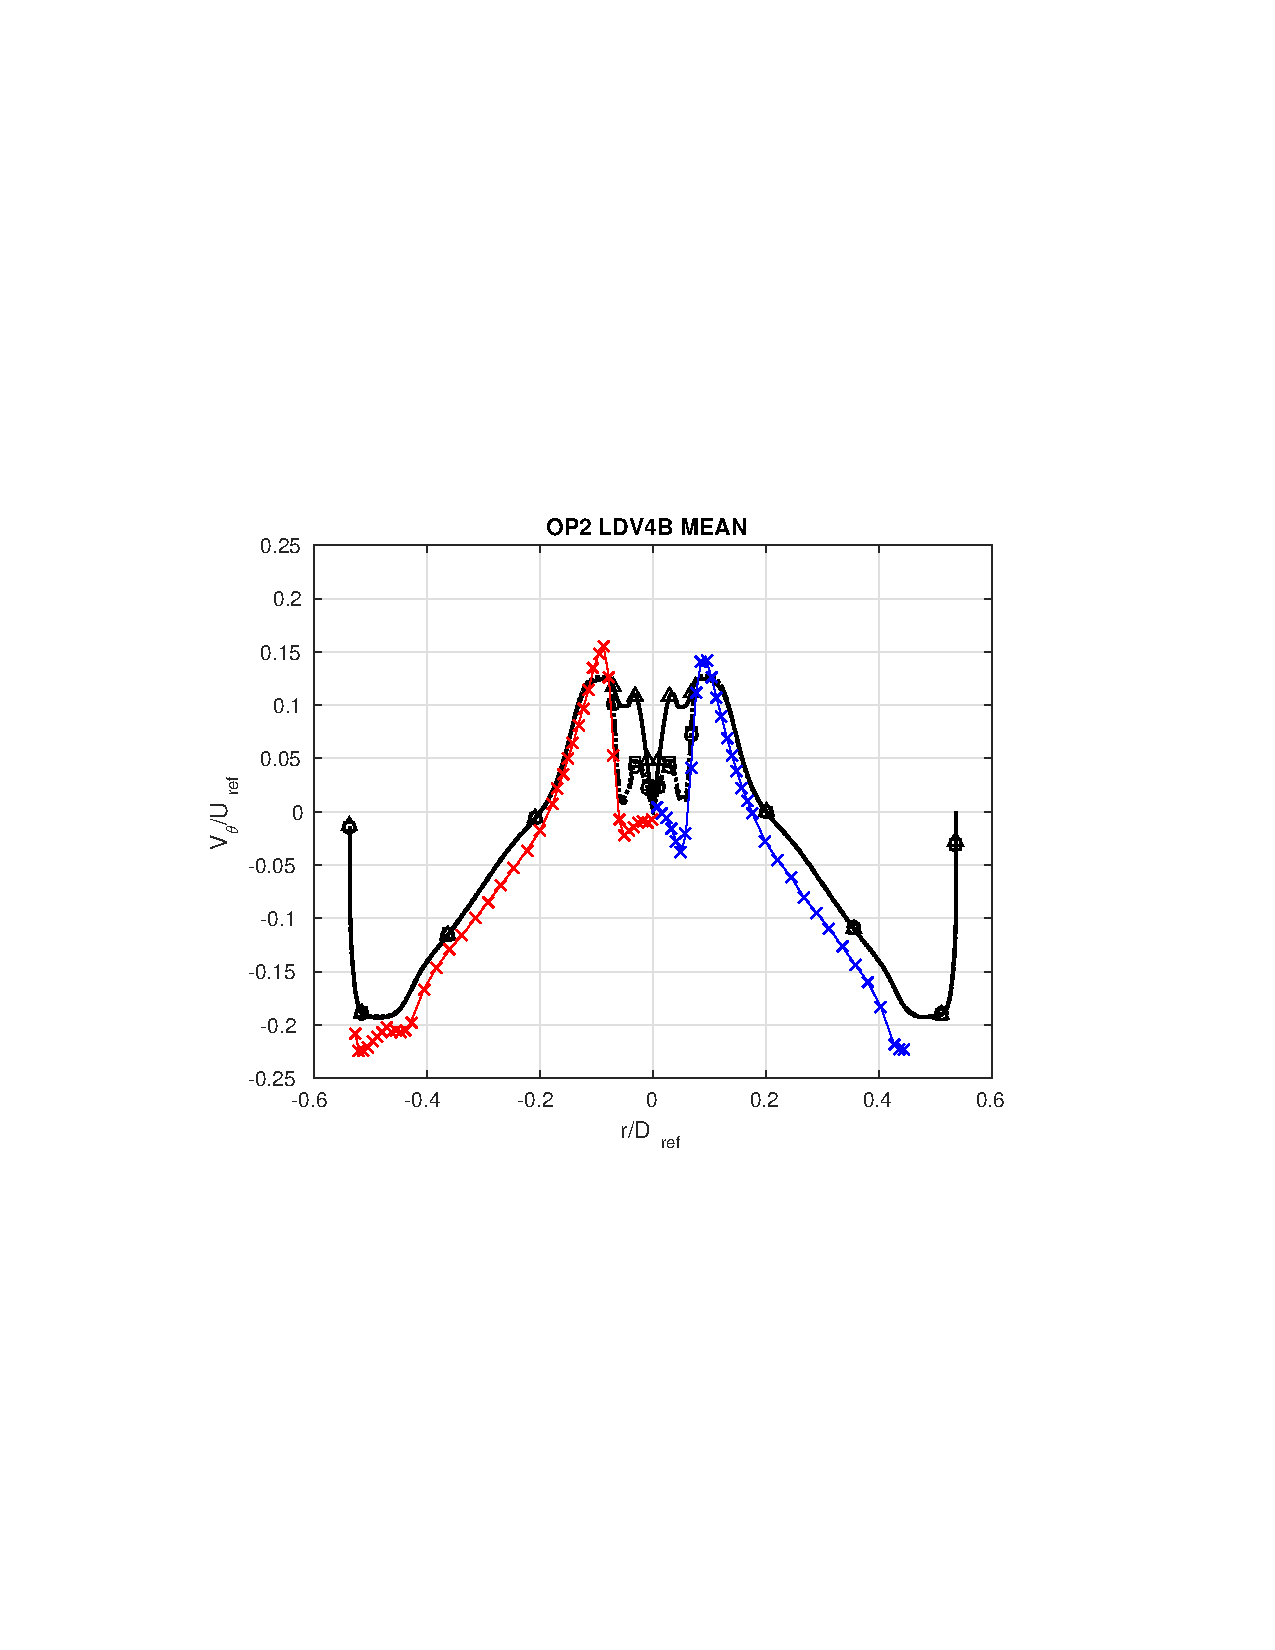
\includegraphics[clip=true, trim= 3.0cm 8.0cm 4.0cm 8.0cm,width=0.98\linewidth]{./figures/bulbt/4BY0/14m/multi_plan4BY0_BulbT_op2_uncert_X_v}} \\
     \subfigure[]{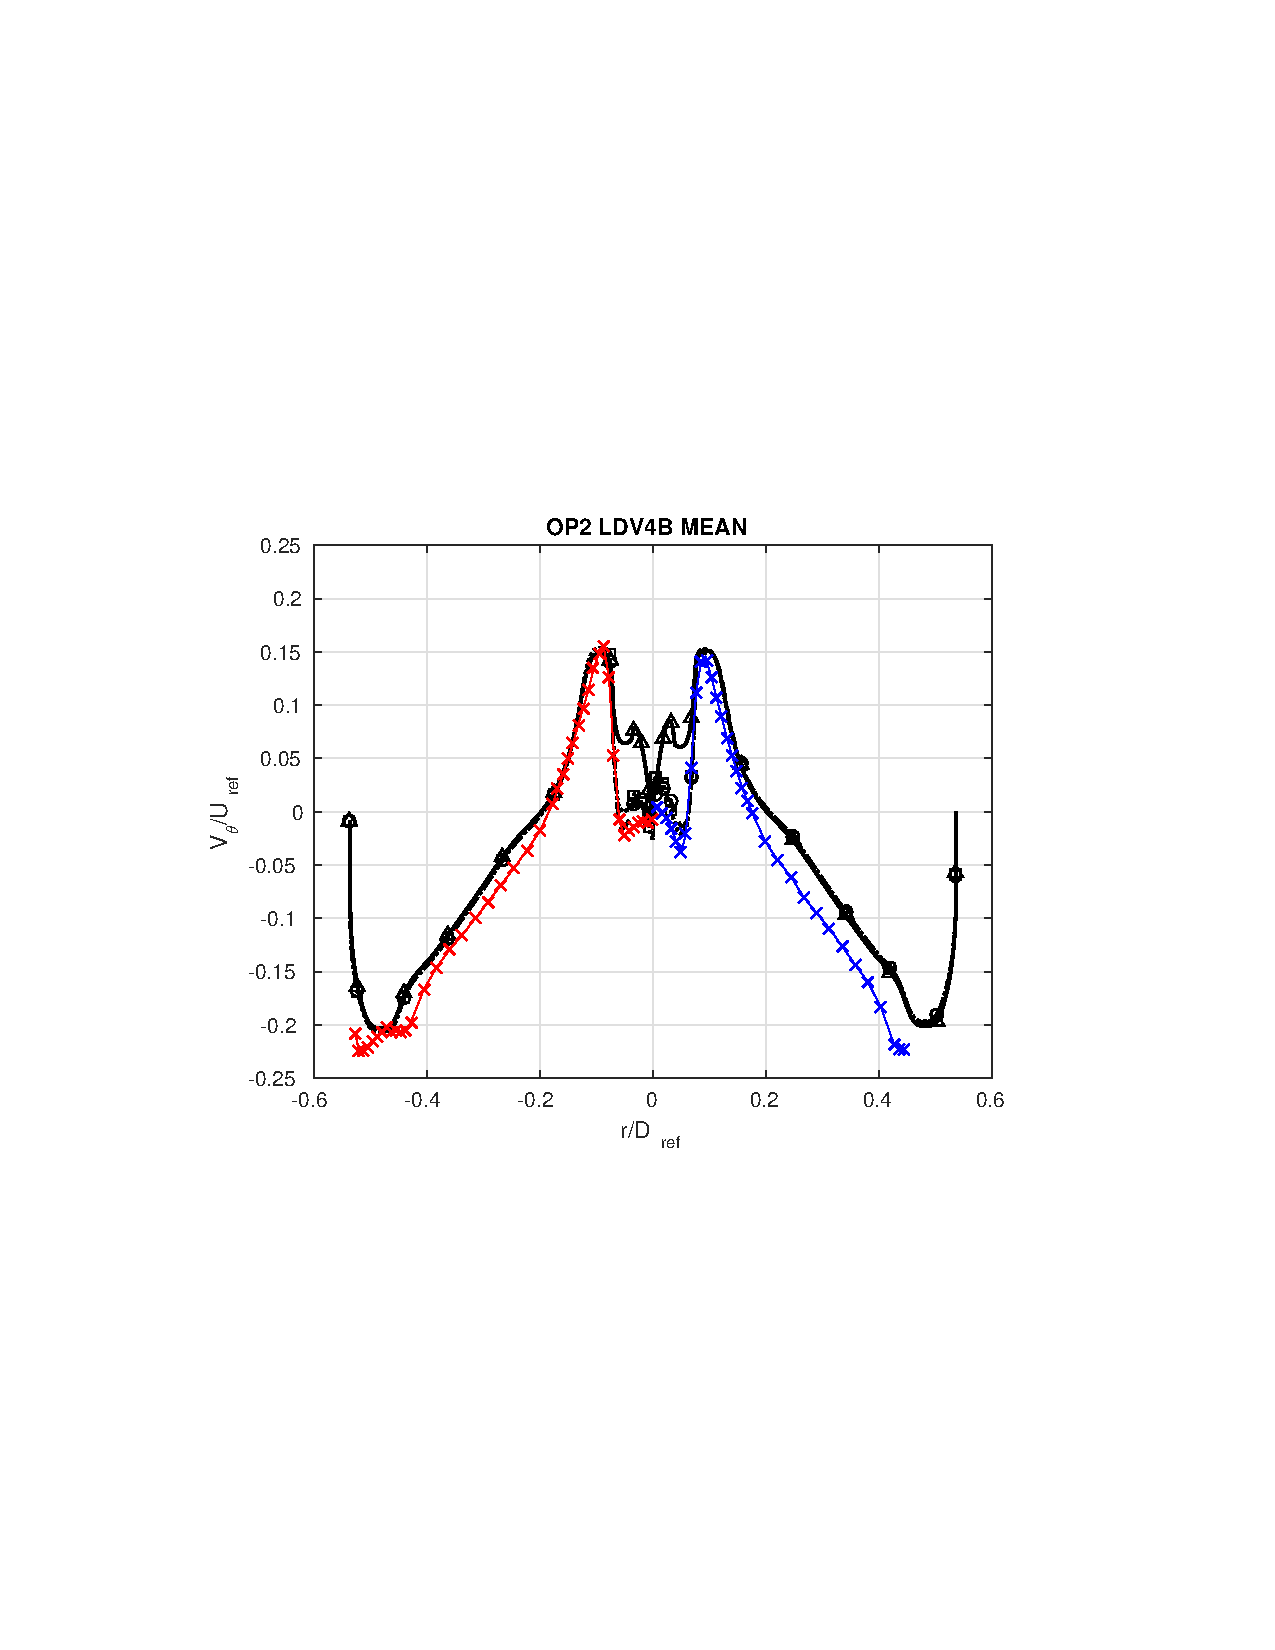
\includegraphics[clip=true, trim= 3.0cm 8.0cm 4.0cm 8.0cm,width=0.98\linewidth]{./figures/bulbt/4BY0/50m/multi_plan4BY0_BulbT_op2_uncert_X_v}}     
     \caption{Circumferential velocity profiles at 4BY0 on (a)3M (b)14M (c)50M grid. (MUSCL: \mline; EDDY: \eline; EDDY-P: \epline; EXP Az0: \bluecrx; EXP Az180: \redcrx.)}
     \label{v}    
\end{figure}
%%%%%%%%%%%%%%%%%%%%%%%%%%%%%%%%%%%%%%%%%%%%%%%%%%%%%%%%%%%%%%%%
\begin{figure}[t]  
\centering
     \subfigure[]{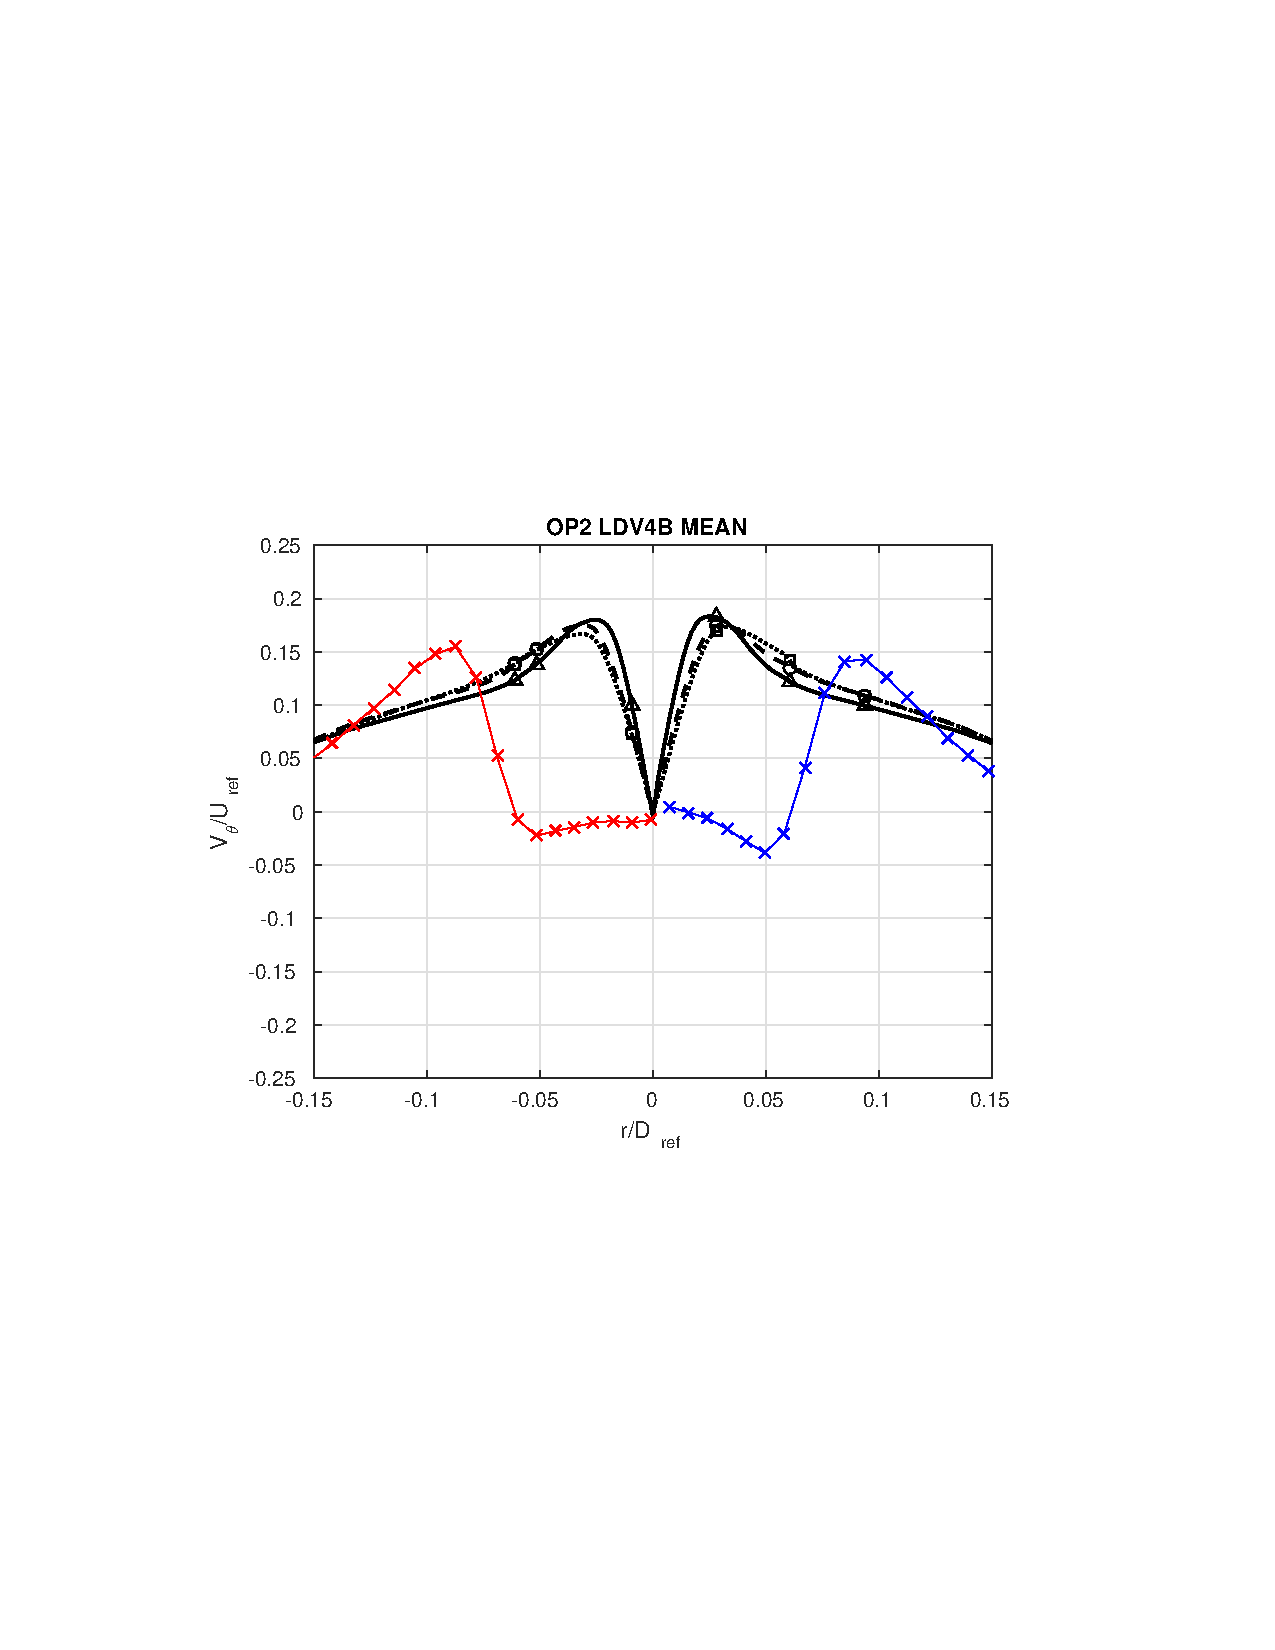
\includegraphics[clip=true, trim= 3.0cm 8.0cm 4.0cm 8.0cm,width=0.98\linewidth]{./figures/bulbt/4BY0/3m/zoom_multi_plan4BY0_BulbT_op2_uncert_X_v}} \\             
     \subfigure[]{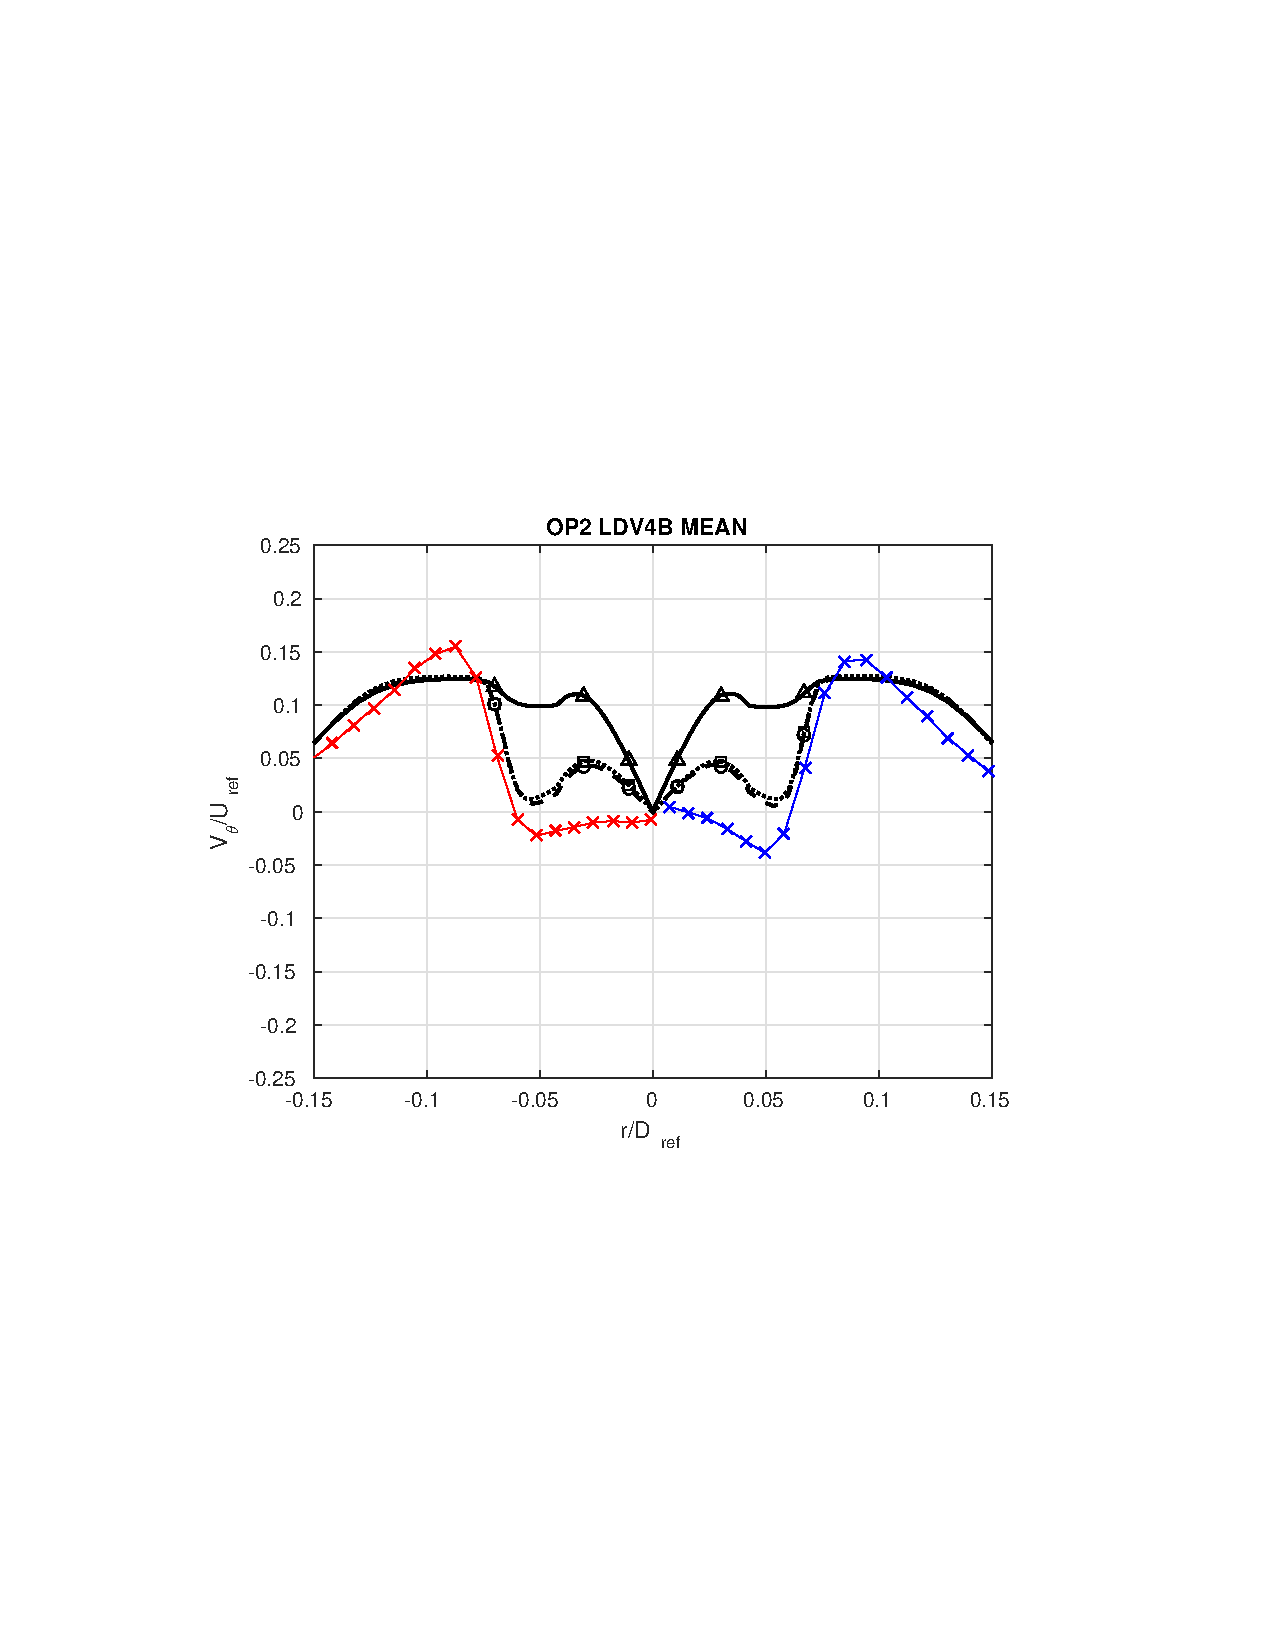
\includegraphics[clip=true, trim= 3.0cm 8.0cm 4.0cm 8.0cm,width=0.98\linewidth]{./figures/bulbt/4BY0/14m/zoom_multi_plan4BY0_BulbT_op2_uncert_X_v}} \\
     \subfigure[]{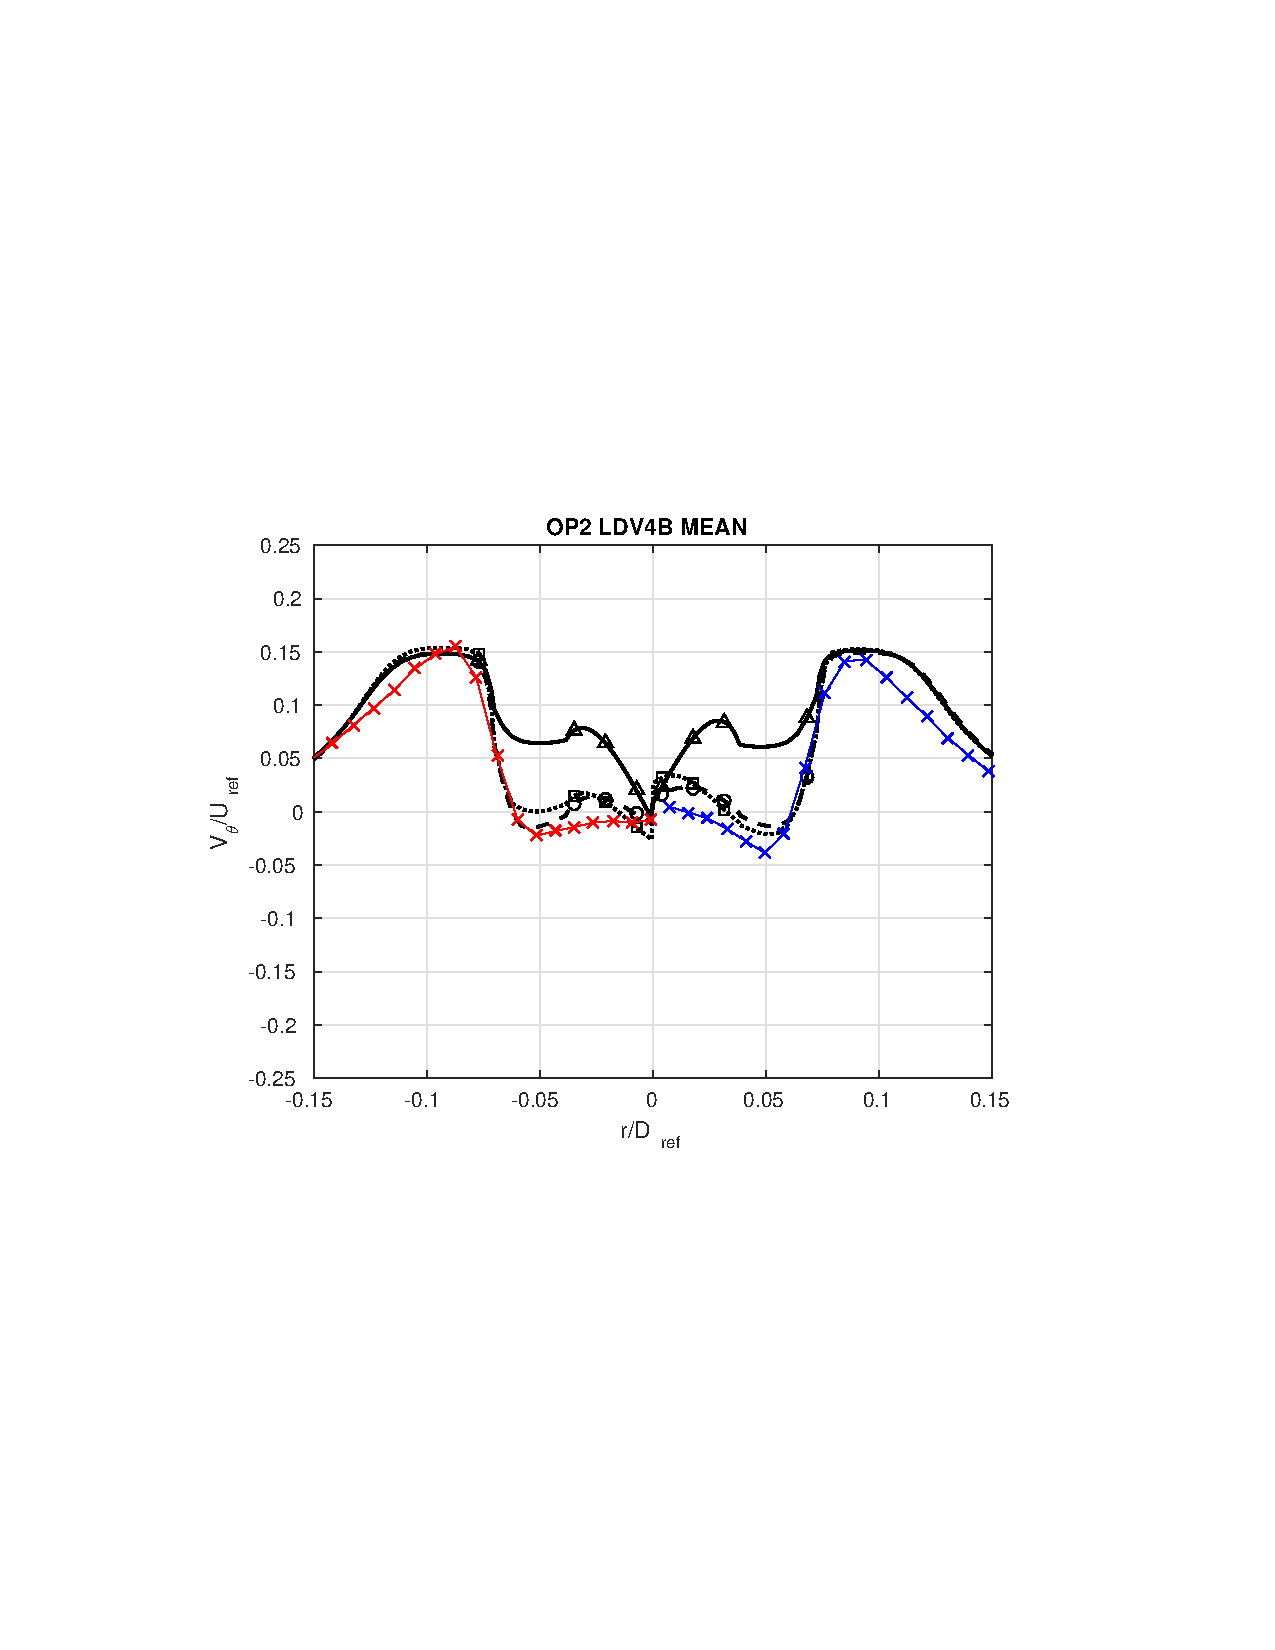
\includegraphics[clip=true, trim= 3.0cm 8.0cm 4.0cm 8.0cm,width=0.98\linewidth]{./figures/bulbt/4BY0/50m/zoom_multi_plan4BY0_BulbT_op2_uncert_X_v}}        
     \caption{Zoom-in view of circumferential velocity profiles at 4BY0 on (a)3M (b)14M (c)50M grid. (MUSCL: \mline; EDDY: \eline; EDDY-P: \epline; EXP Az0: \bluecrx; EXP Az180: \redcrx.)}
     \label{zv} 
\end{figure}
%%%%%%%%%%%%%%%%%%%%%%%%%%%%%%%%%%%%%%%%%%%%%%%%%%%%%%%%%%%%%%%%
%%%%%%%%%%%%%%%%%%%%%%%%%%%%%%%%%%%%%%%%%%%%%%%%%%%%%%%%%%%%%%%%
\begin{figure}[t]  
\centering
     \subfigure[]{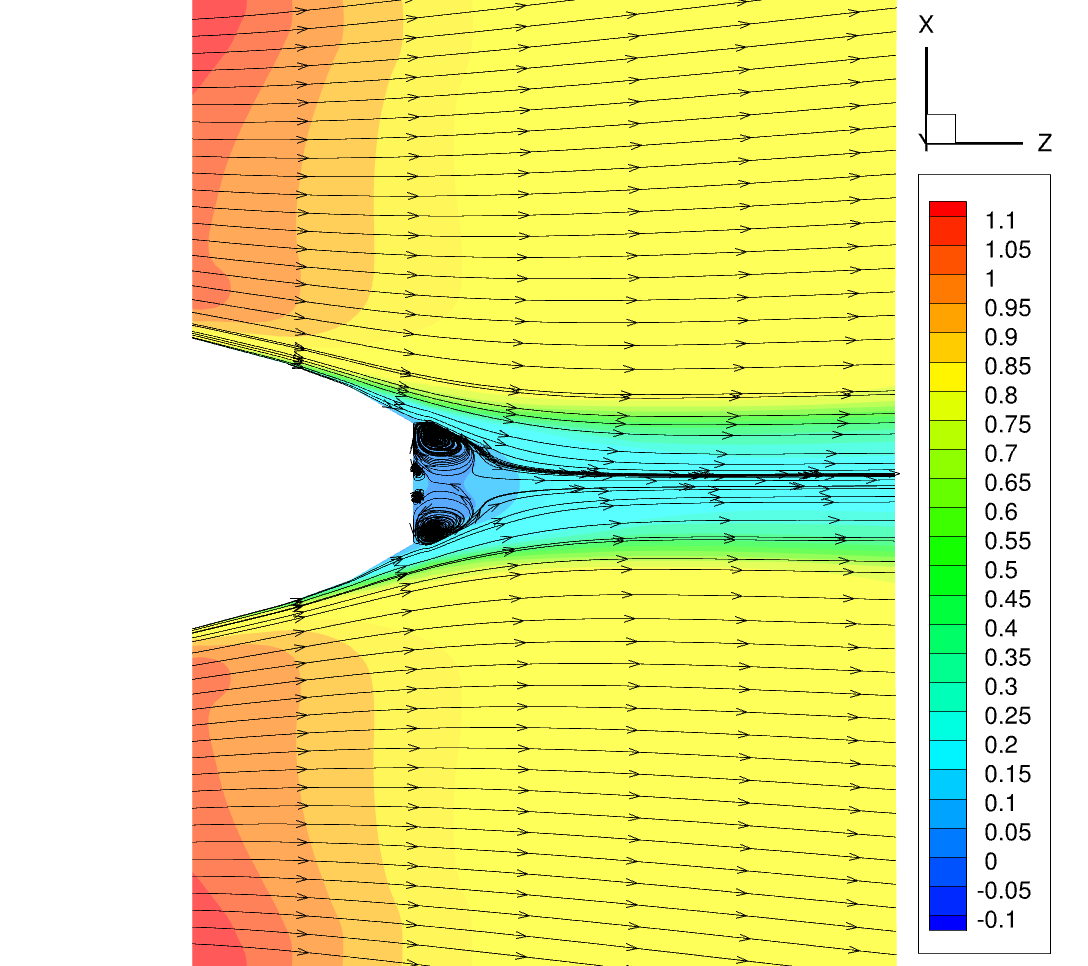
\includegraphics[clip=true, trim= 6.25cm 0.25cm 0.25cm 0.25cm,width=0.85\linewidth]{./figures/bulbt/w-contours-y0/14m-m}} \\            
     \subfigure[]{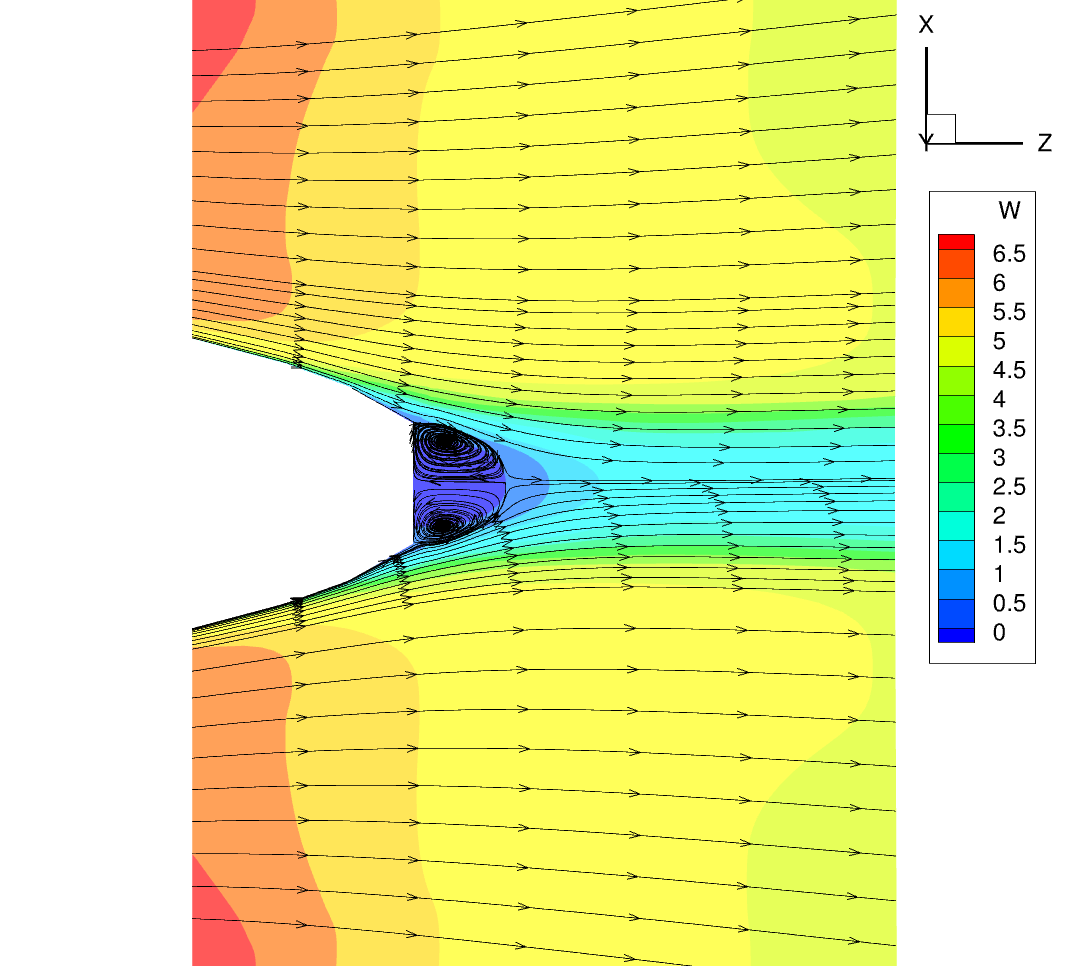
\includegraphics[clip=true, trim= 6.25cm 0.25cm 0.25cm 0.25cm,width=0.85\linewidth]{./figures/bulbt/w-contours-y0/14m-e}} \\
     \subfigure[]{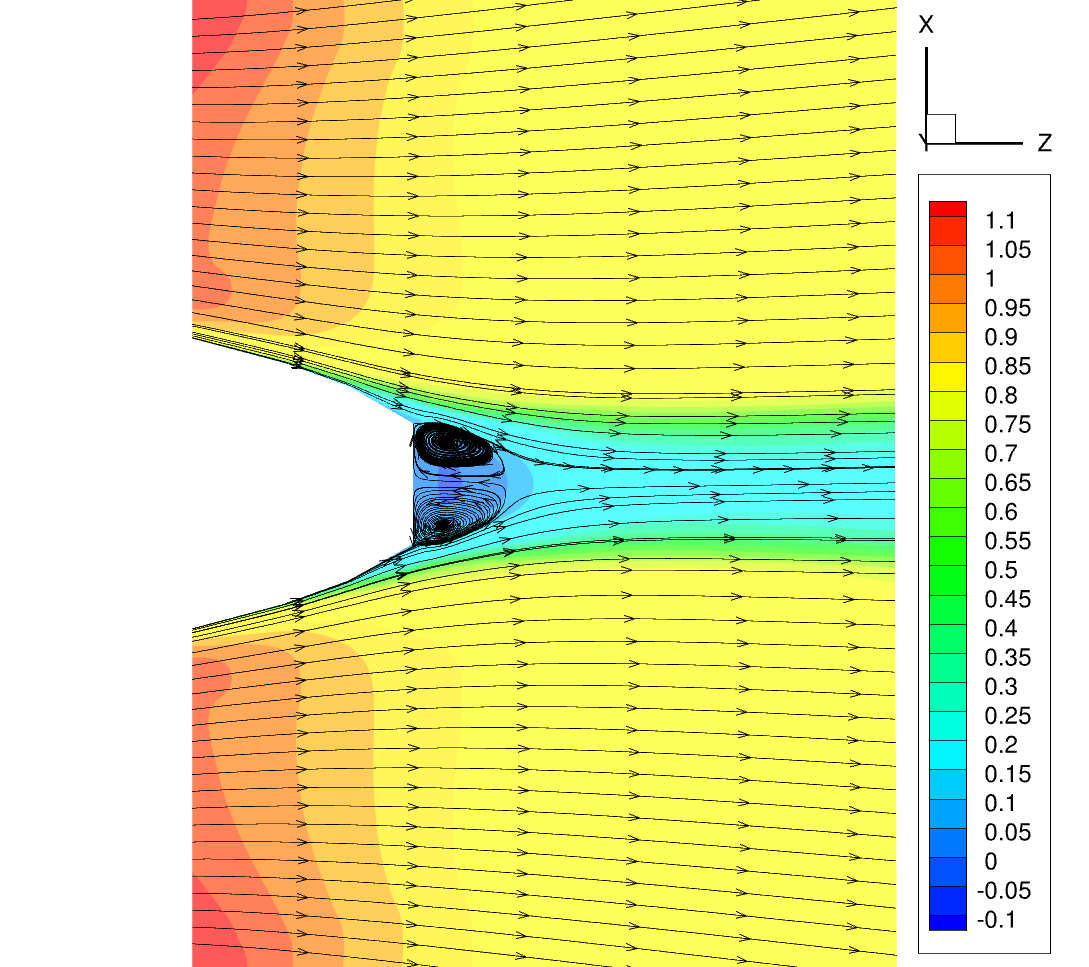
\includegraphics[clip=true, trim= 6.25cm 0.25cm 0.25cm 0.25cm,width=0.85\linewidth]{./figures/bulbt/w-contours-y0/14m-ep}}        
     \caption{Contours of axial velocity and two dimensional streamlines on 14M grid computed by (a)MUSCL (b)EDDY (c)EDDY-P scheme.}
     \label{w1} 
\end{figure}
%%%%%%%%%%%%%%%%%%%%%%%%%%%%%%%%%%%%%%%%%%%%%%%%%%%%%%%%%%%%%%%%
%%%%%%%%%%%%%%%%%%%%%%%%%%%%%%%%%%%%%%%%%%%%%%%%%%%%%%%%%%%%%%%%
\begin{figure}[t]  
\centering
     \subfigure[]{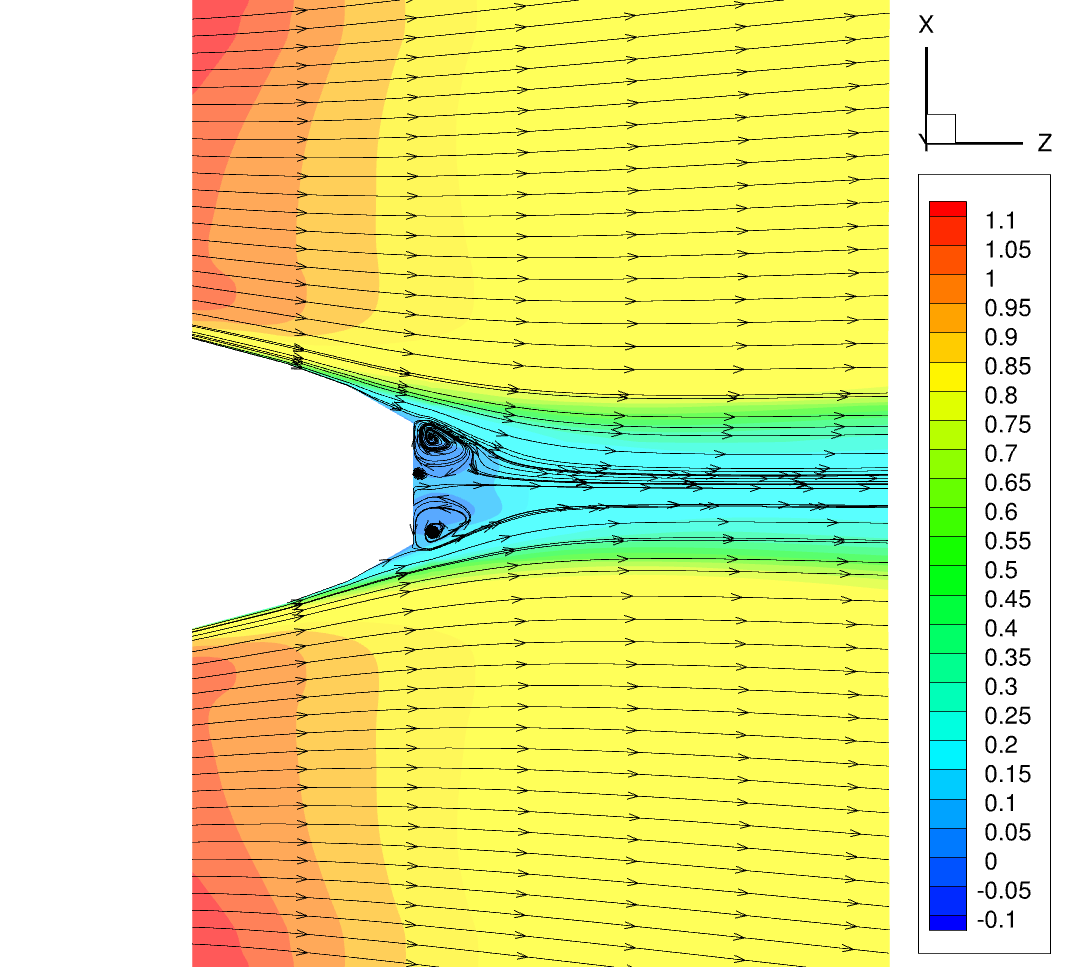
\includegraphics[clip=true, trim= 6.25cm 0.25cm 0.25cm 0.25cm,width=0.85\linewidth]{./figures/bulbt/w-contours-y0/50m-m}} \\            
     \subfigure[]{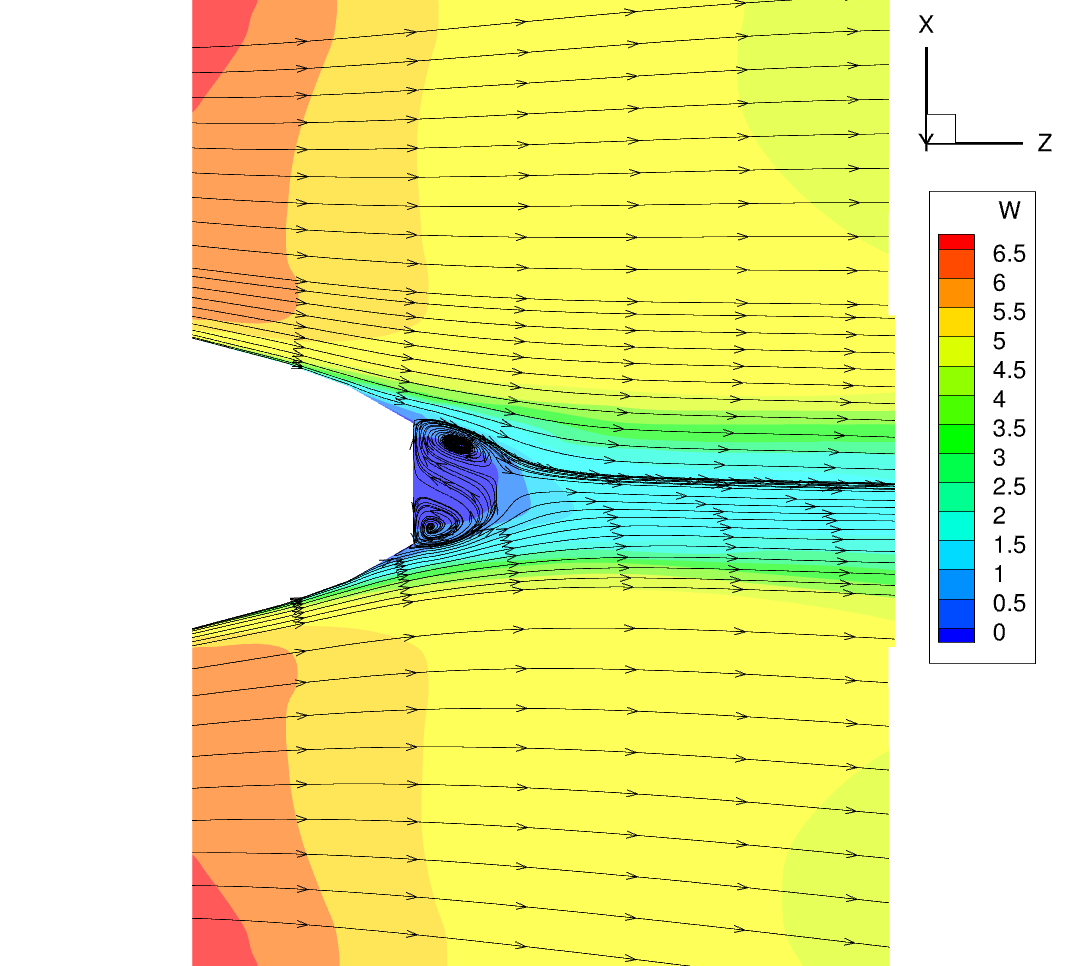
\includegraphics[clip=true, trim= 6.25cm 0.25cm 0.25cm 0.25cm,width=0.85\linewidth]{./figures/bulbt/w-contours-y0/50m-e}} \\
     \subfigure[]{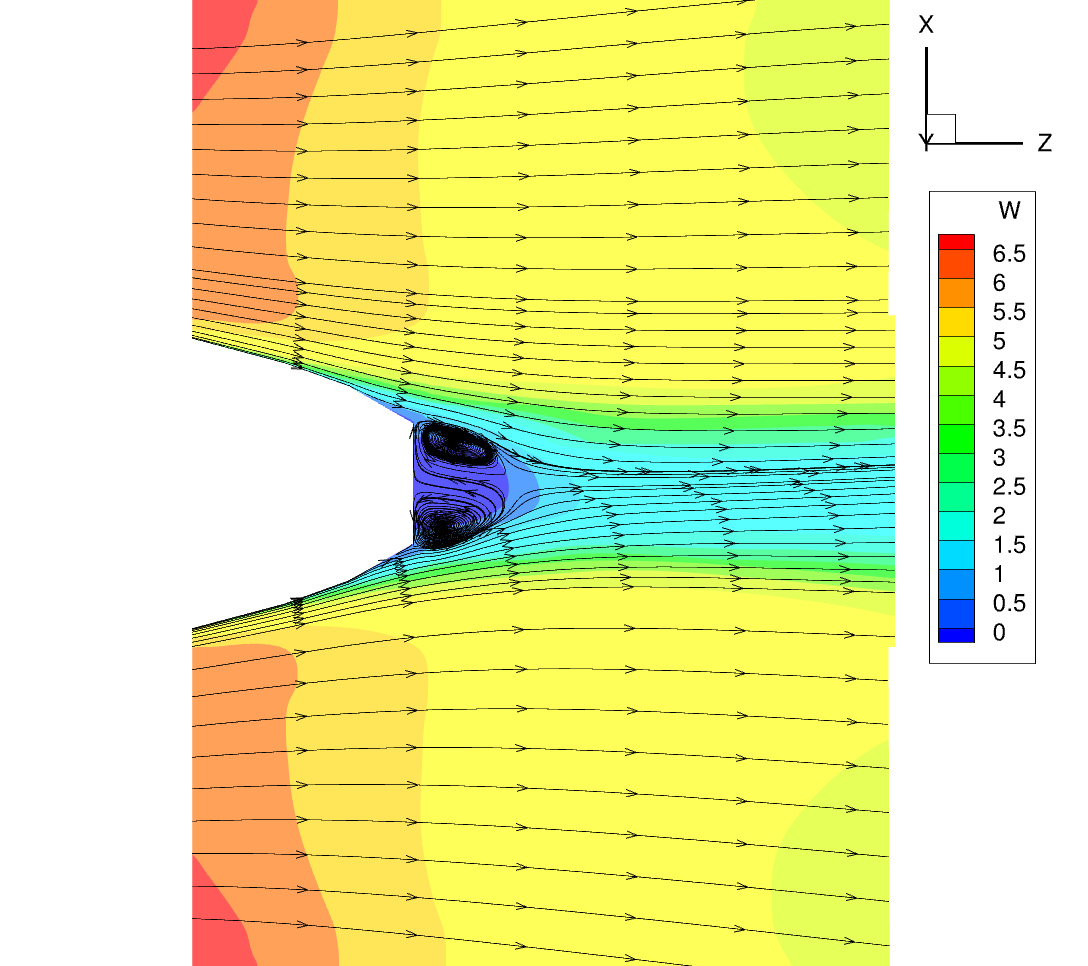
\includegraphics[clip=true, trim= 6.25cm 0.25cm 0.25cm 0.25cm,width=0.85\linewidth]{./figures/bulbt/w-contours-y0/50m-ep}}        
     \caption{Contours of axial velocity and two dimensional streamlines on 50M grid computed by (a)MUSCL (b)EDDY (c)EDDY-P scheme.}
     \label{w2} 
\end{figure}
%%%%%%%%%%%%%%%%%%%%%%%%%%%%%%%%%%%%%%%%%%%%%%%%%%%%%%%%%%%%%%%%
%%%%%%%%%%%%%%%%%%%%%%%%%%%%%%%%%%%%%%%%%%%%%%%%%%%%%%%%%%%%%%%%
%%%%%%%%%%%%%%%%%%%%%%%%%%%%%%%%%%%%%%%%%%%%%%%%%%%%%%%%%%%%%%%%
%%%%%%%%%%%%%%%%%%%%%%%%%%%%%%%%%%%%%%%%%%%%%%%%%%%%%%%%%%%%%%%%
\begin{figure}[t]  
\centering
     \subfigure[]{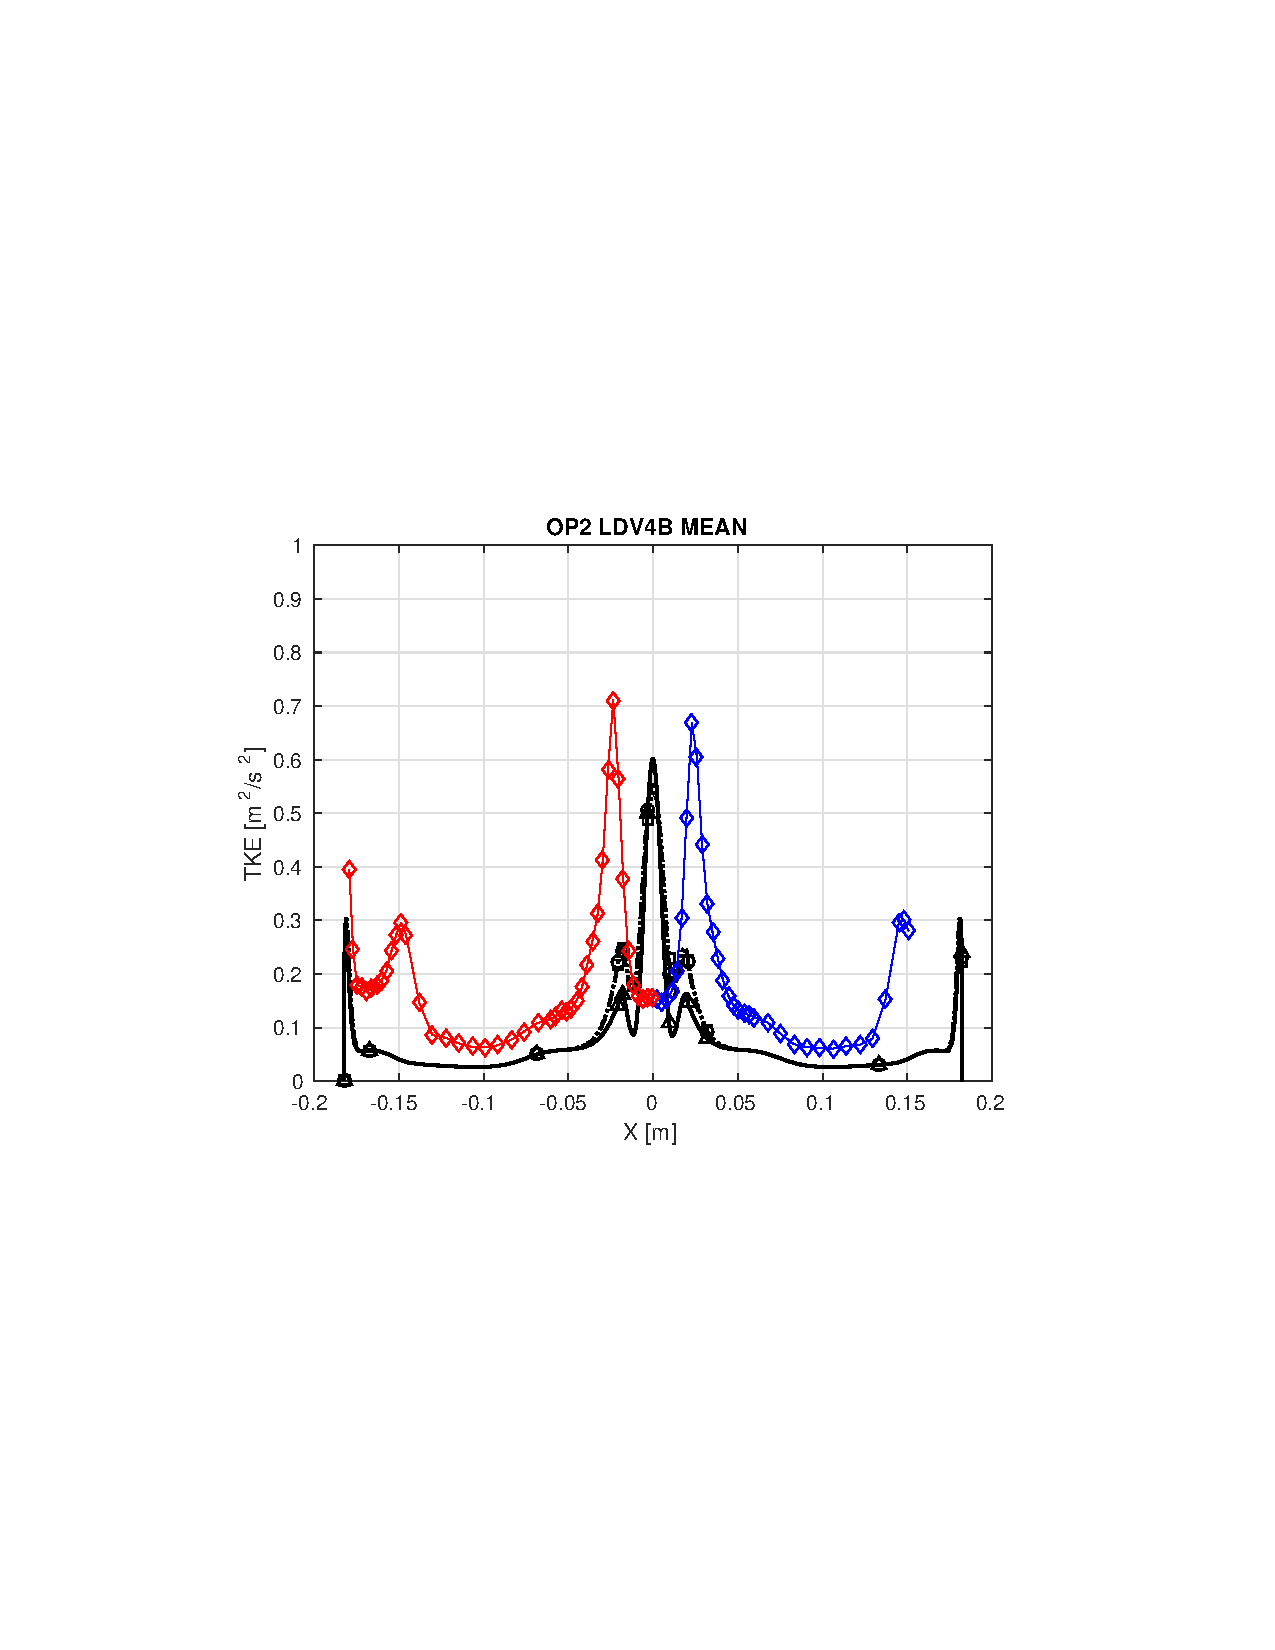
\includegraphics[clip=true, trim= 3.0cm 8.0cm 4.0cm 8.0cm,width=0.98\linewidth]{./figures/bulbt/4BY0/3m/multi_plan4BY0_BulbT_op2_Tke_X}} \\             
     \subfigure[]{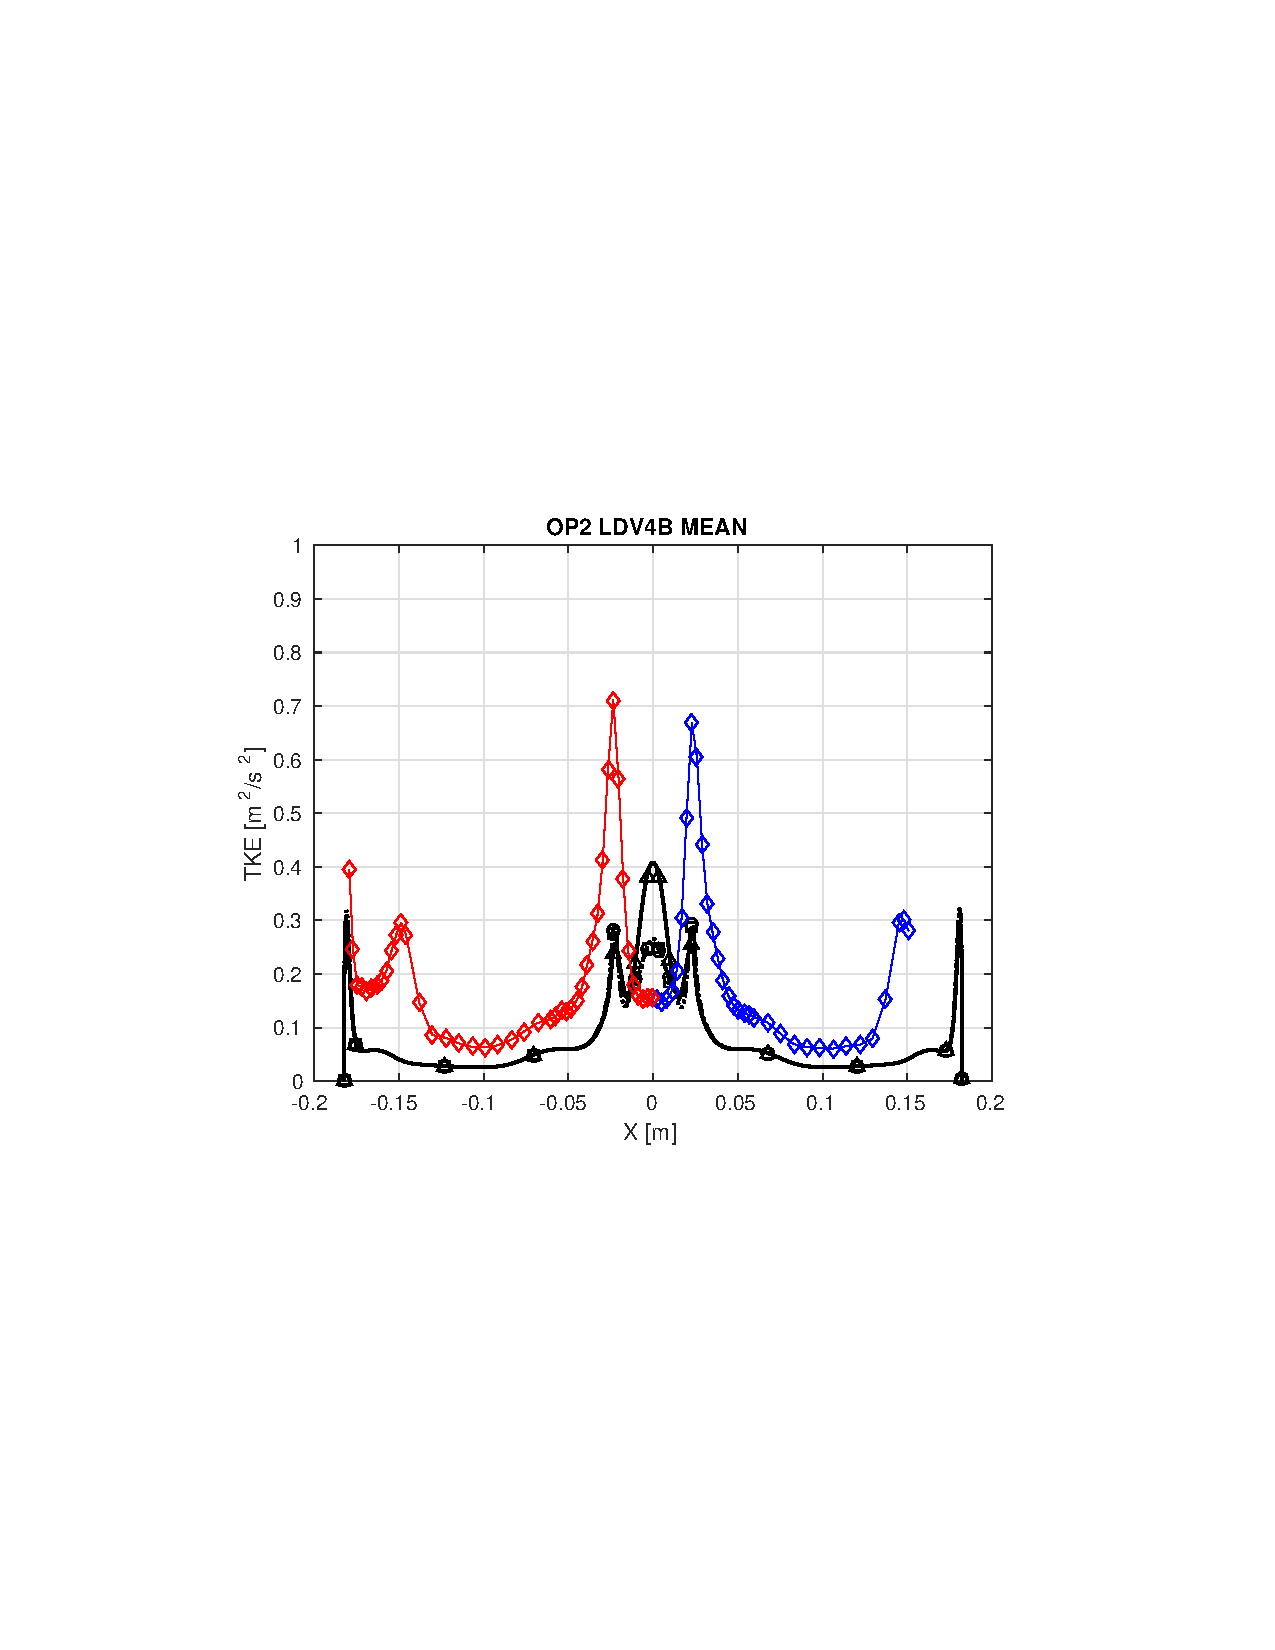
\includegraphics[clip=true, trim= 3.0cm 8.0cm 4.0cm 8.0cm,width=0.98\linewidth]{./figures/bulbt/4BY0/14m/multi_plan4BY0_BulbT_op2_Tke_X}} \\
     \subfigure[]{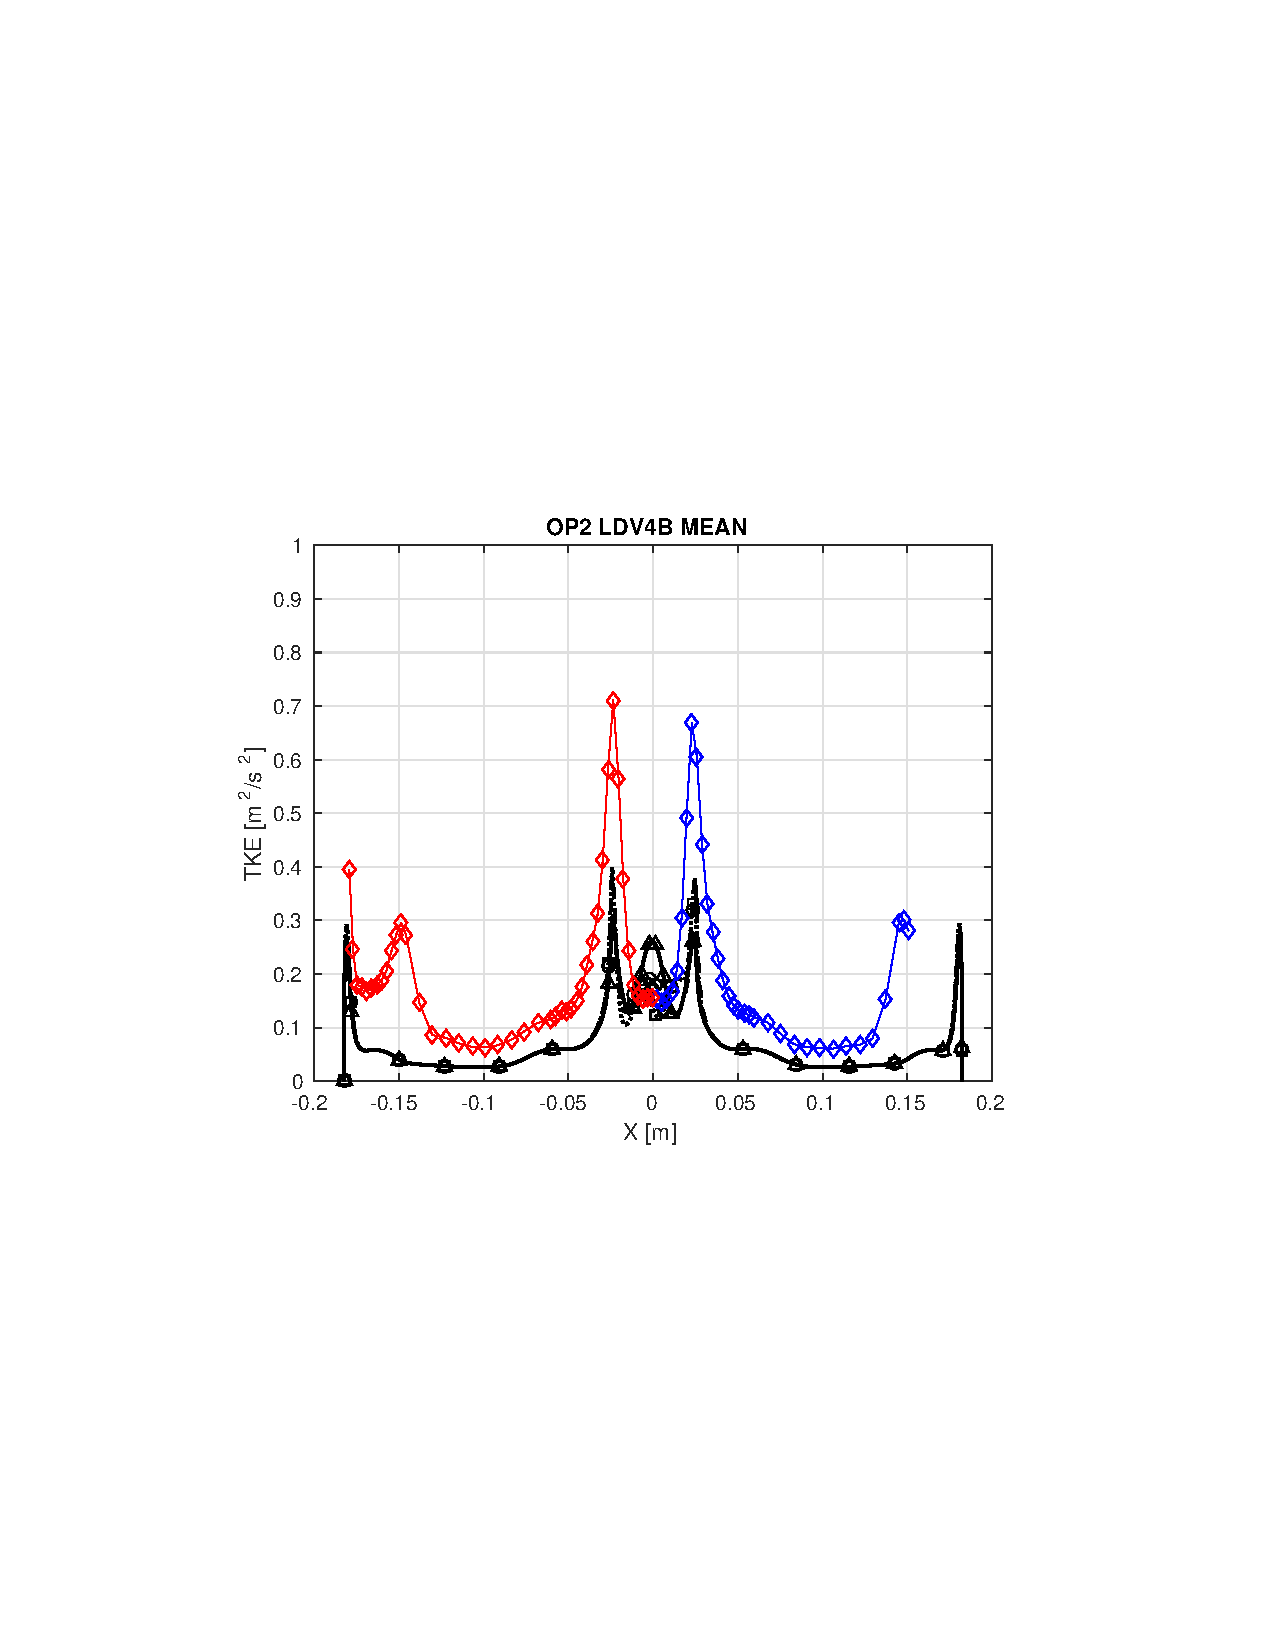
\includegraphics[clip=true, trim= 3.0cm 8.0cm 4.0cm 8.0cm,width=0.98\linewidth]{./figures/bulbt/4BY0/50m/multi_plan4BY0_BulbT_op2_Tke_X}}        
     \caption{TKE profiles at 4BY0 on (a)3M (b)14M (c)50M grid.  (MUSCL: \mline; EDDY: \eline; EDDY-P: \epline; EXP Az0: \bluediam; EXP Az180: \reddiam.)}
     \label{tke} 
\end{figure}
%%%%%%%%%%%%%%%%%%%%%%%%%%%%%%%%%%%%%%%%%%%%%%%%%%%%%%%%%%%%%%%%
\begin{figure}[t]  
\centering
     \subfigure[]{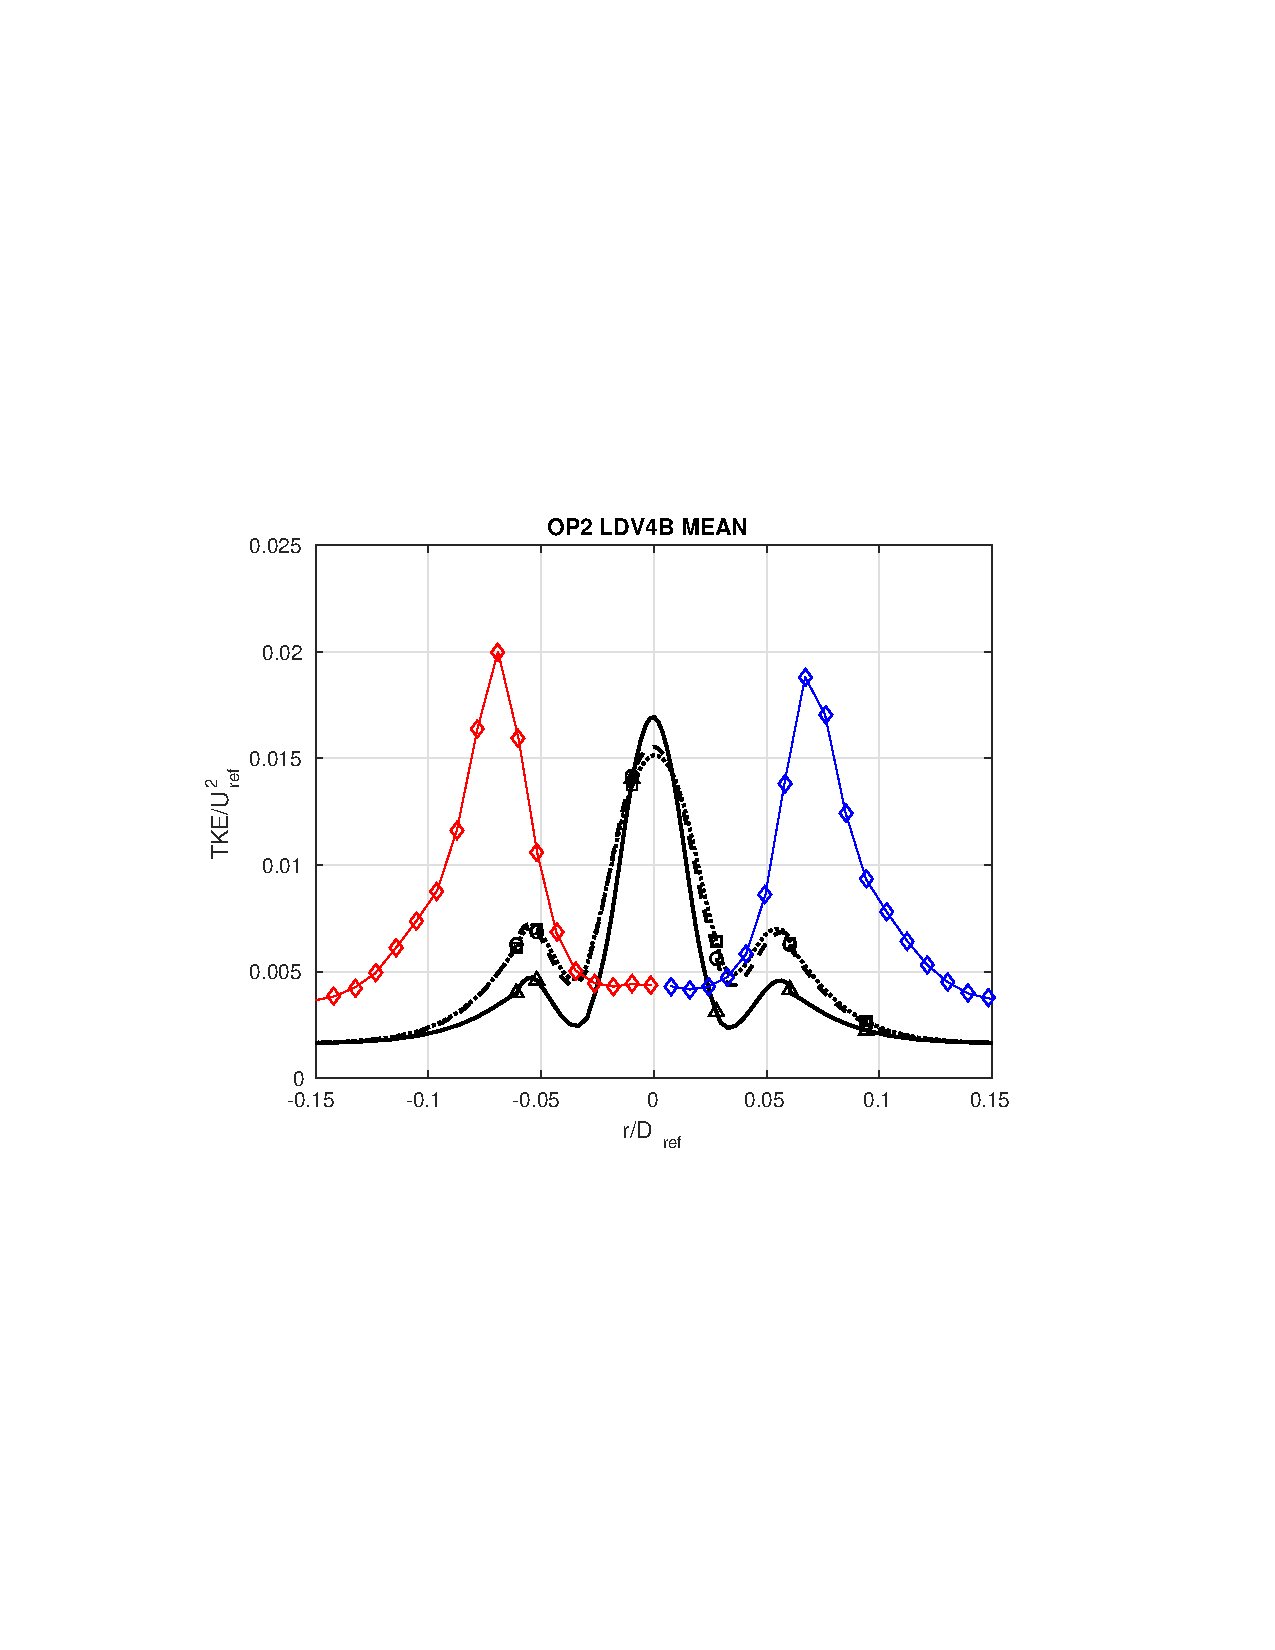
\includegraphics[clip=true, trim= 3.0cm 8.0cm 4.0cm 8.0cm,width=0.98\linewidth]{./figures/bulbt/4BY0/3m/zoom_multi_plan4BY0_BulbT_op2_Tke_X}} \\             
     \subfigure[]{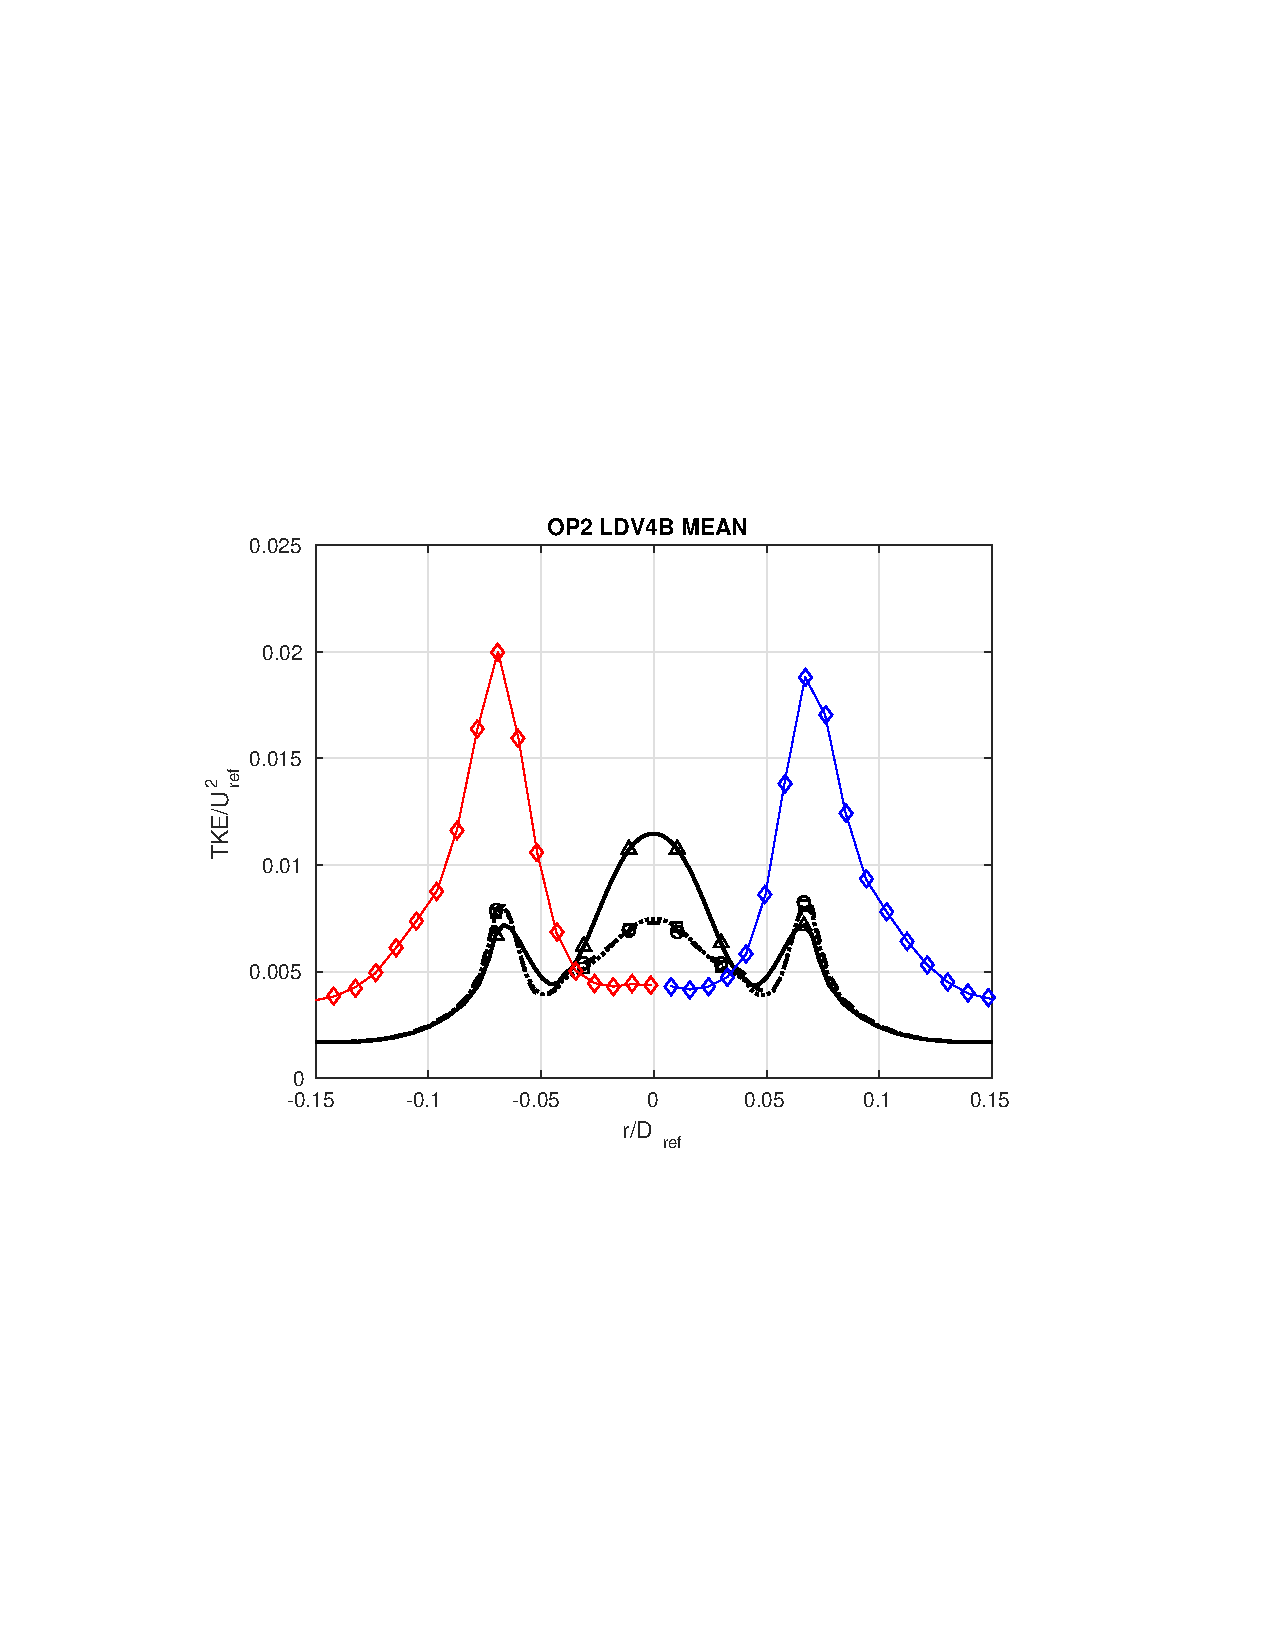
\includegraphics[clip=true, trim= 3.0cm 8.0cm 4.0cm 8.0cm,width=0.98\linewidth]{./figures/bulbt/4BY0/14m/zoom_multi_plan4BY0_BulbT_op2_Tke_X}} \\
     \subfigure[]{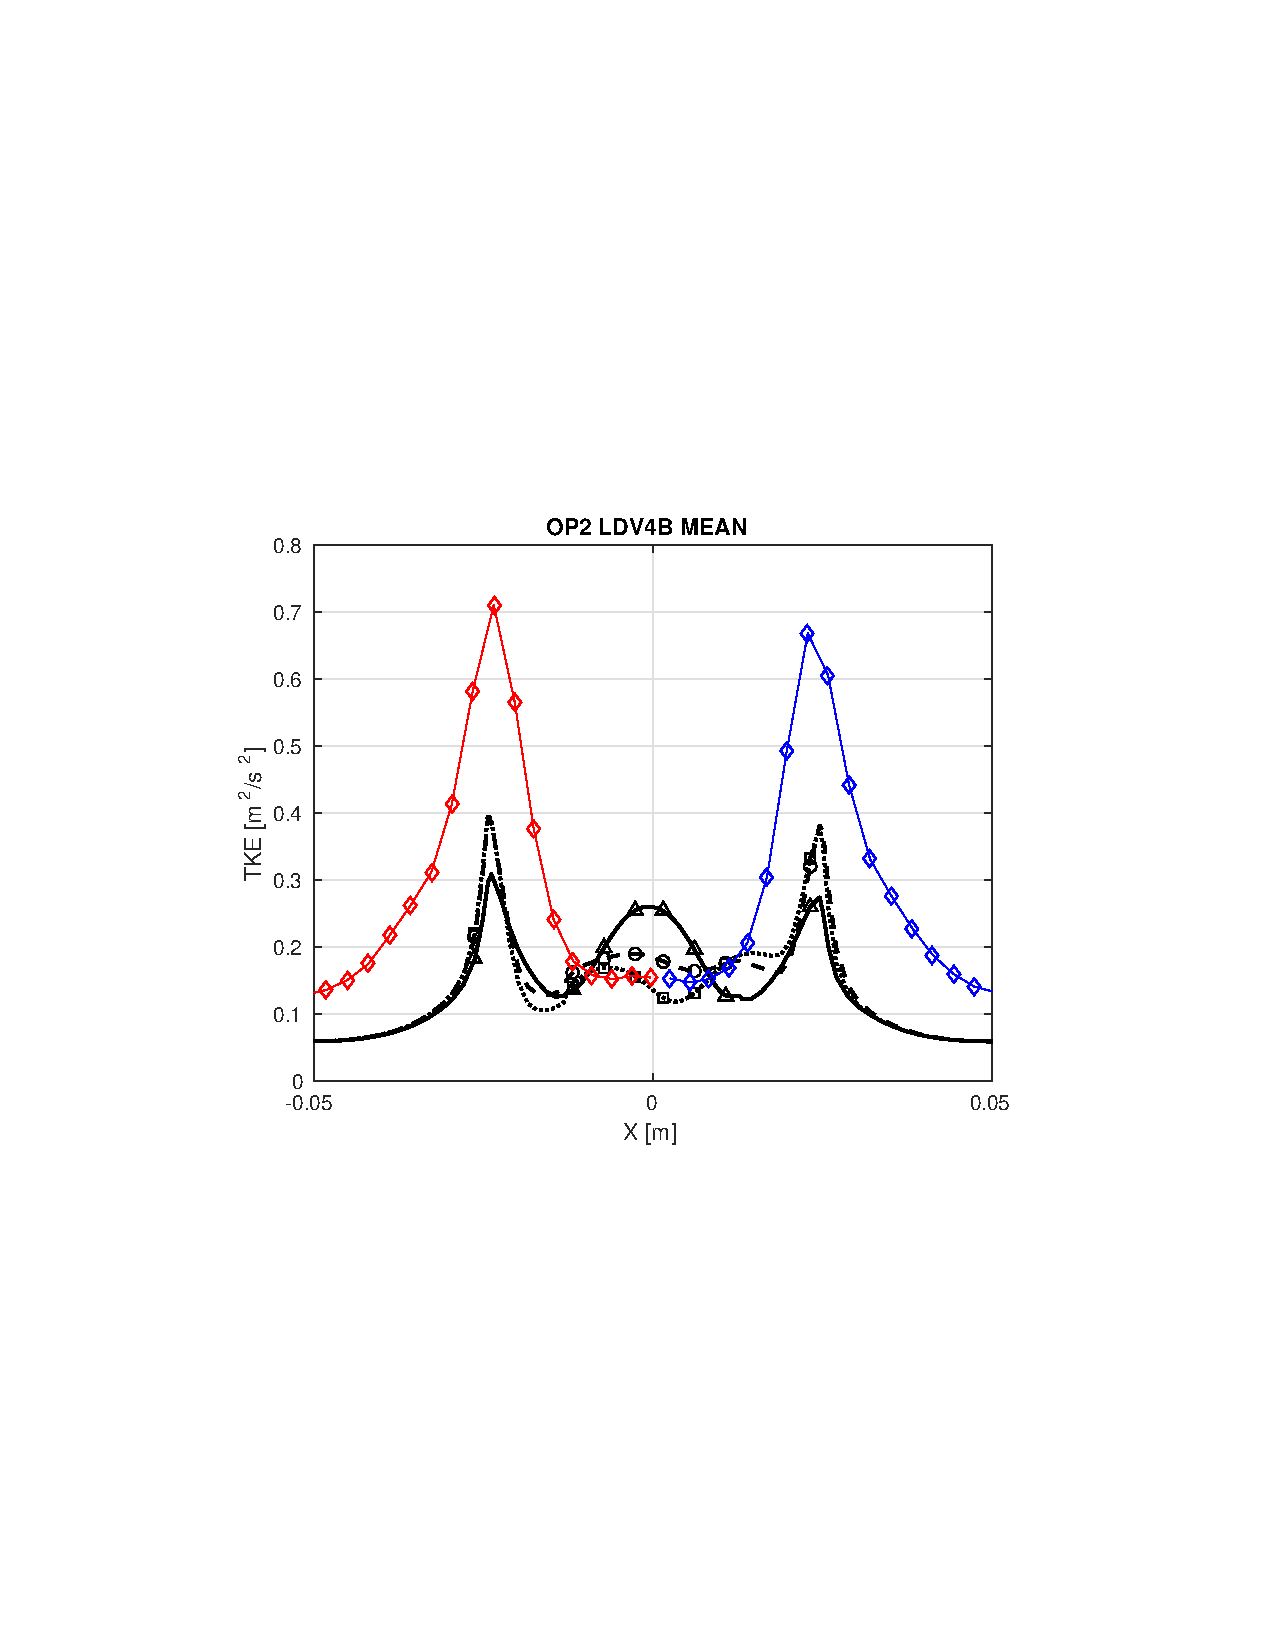
\includegraphics[clip=true, trim= 3.0cm 8.0cm 4.0cm 8.0cm,width=0.98\linewidth]{./figures/bulbt/4BY0/50m/zoom_multi_plan4BY0_BulbT_op2_Tke_X}}       
     \caption{Zoom-in view of TKE profiles at 4BY0 on (a)3M (b)14M (c)50M grid. (MUSCL: \mline; EDDY: \eline; EDDY-P: \epline; EXP Az0: \bluediam; EXP Az180: \reddiam.)}
     \label{ztke} 
\end{figure}
%%%%%%%%%%%%%%%%%%%%%%%%%%%%%%%%%%%%%%%%%%%%%%%%%%%%%%%%%%%%%%%%
%%%%%%%%%%%%%%%%%%%%%%%%%%%%%%%%%%%%%%%%%%%%%%%%%%%%%%%%%%%%%%%%
%%%%%%%%%%%%%%%%%%%%%%%%%%%%%%%%%%%%%%%%%%%%%%%%%%%%%%%%%%%%%%%%
%%%%%%%%%%%%%%%%%%%%%%%%%%%%%%%%%%%%%%%%%%%%%%%%%%%%%%%%%%%%%%%%
%%%%%%%%%%%%%%%%%%%%%%%%%%%%%%%%%%%%%%%%%%%%%%%%%%%%%%%%%%%%%%%%
%%%%%%%%%%%%%%%%%%%%%%%%%%%%%%%%%%%%%%%%%%%%%%%%%%%%%%%%%%%%%%%%
\begin{figure}[t]  
\centering
     \subfigure[]{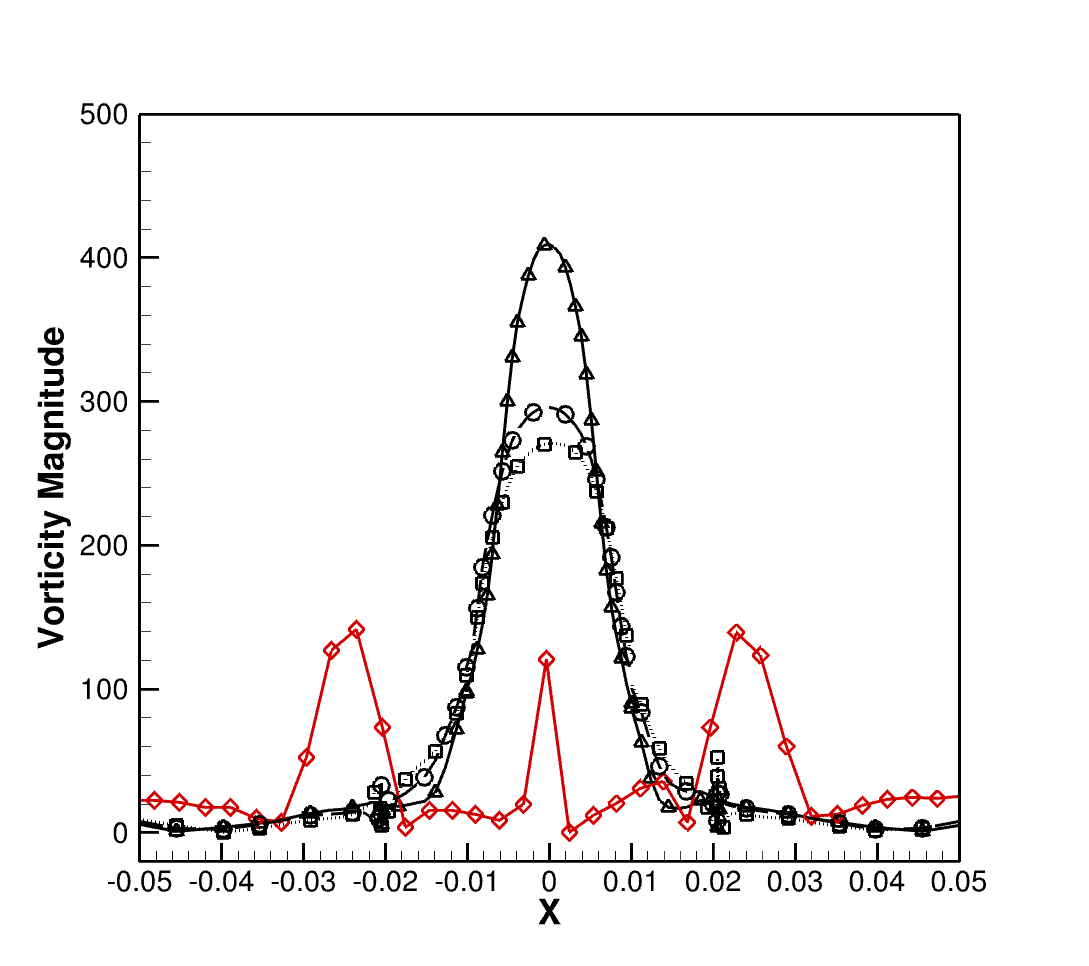
\includegraphics[clip=true, trim= 1.25cm 1.25cm 3.25cm 3.25cm,width=0.98\linewidth]{./figures/bulbt/4by0vo/3m}} \\            
     \subfigure[]{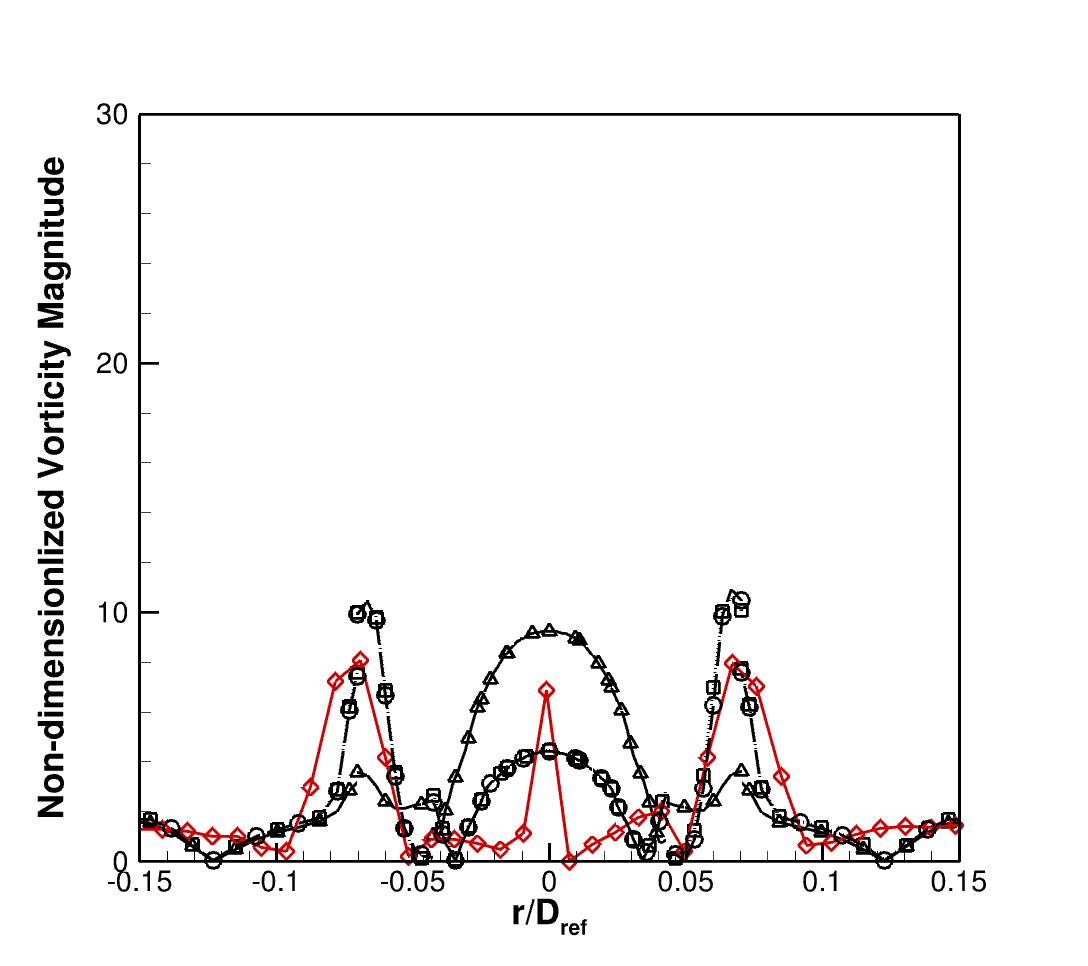
\includegraphics[clip=true, trim= 1.25cm 1.25cm 3.25cm 3.25cm,width=0.98\linewidth]{./figures/bulbt/4by0vo/14m}} \\
     \subfigure[]{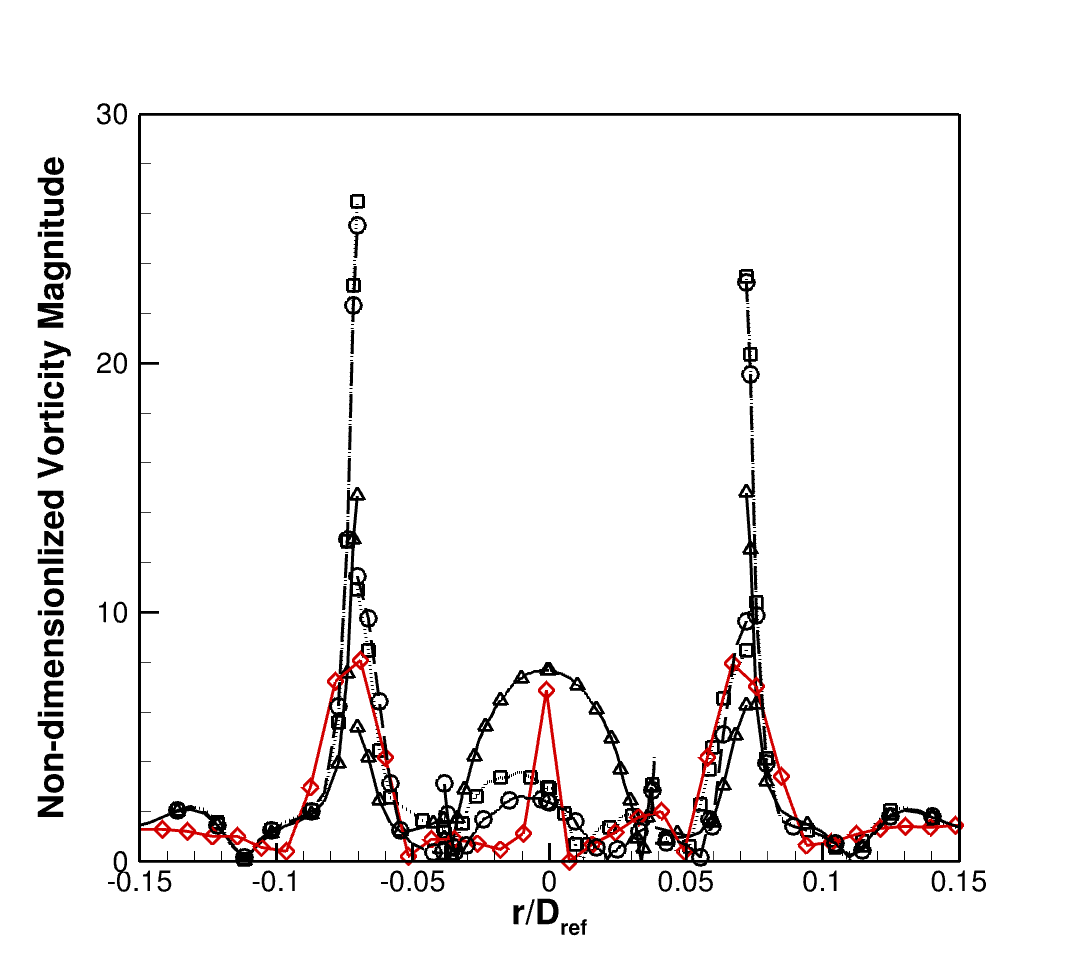
\includegraphics[clip=true, trim= 1.25cm 1.25cm 3.25cm 3.25cm,width=0.98\linewidth]{./figures/bulbt/4by0vo/50m}}        
     \caption{Vorticity magnitude at 4BY0 on (a)3M (b)14M (c)50M grid. (MUSCL: \mline; EDDY: \eline; EDDY-P: \epline; EXP: \exact.)}
     \label{vo} 
\end{figure}
%%%%%%%%%%%%%%%%%%%%%%%%%%%%%%%%%%%%%%%%%%%%%%%%%%%%%%%%%%%%%%%%
%%%%%%%%%%%%%%%%%%%%%%%%%%%%%%%%%%%%%%%%%%%%%%%%%%%%%%%%%%%%%%%%
%%%%%%%%%%%%%%%%%%%%%%%%%%%%%%%%%%%%%%%%%%%%%%%%%%%%%%%%%%%%%%%%
%%%%%%%%%%%%%%%%%%%%%%%%%%%%%%%%%%%%%%%%%%%%%%%%%%%%%%%%%%%%%%%%
\begin{figure}[t]  
\centering
     \subfigure[]{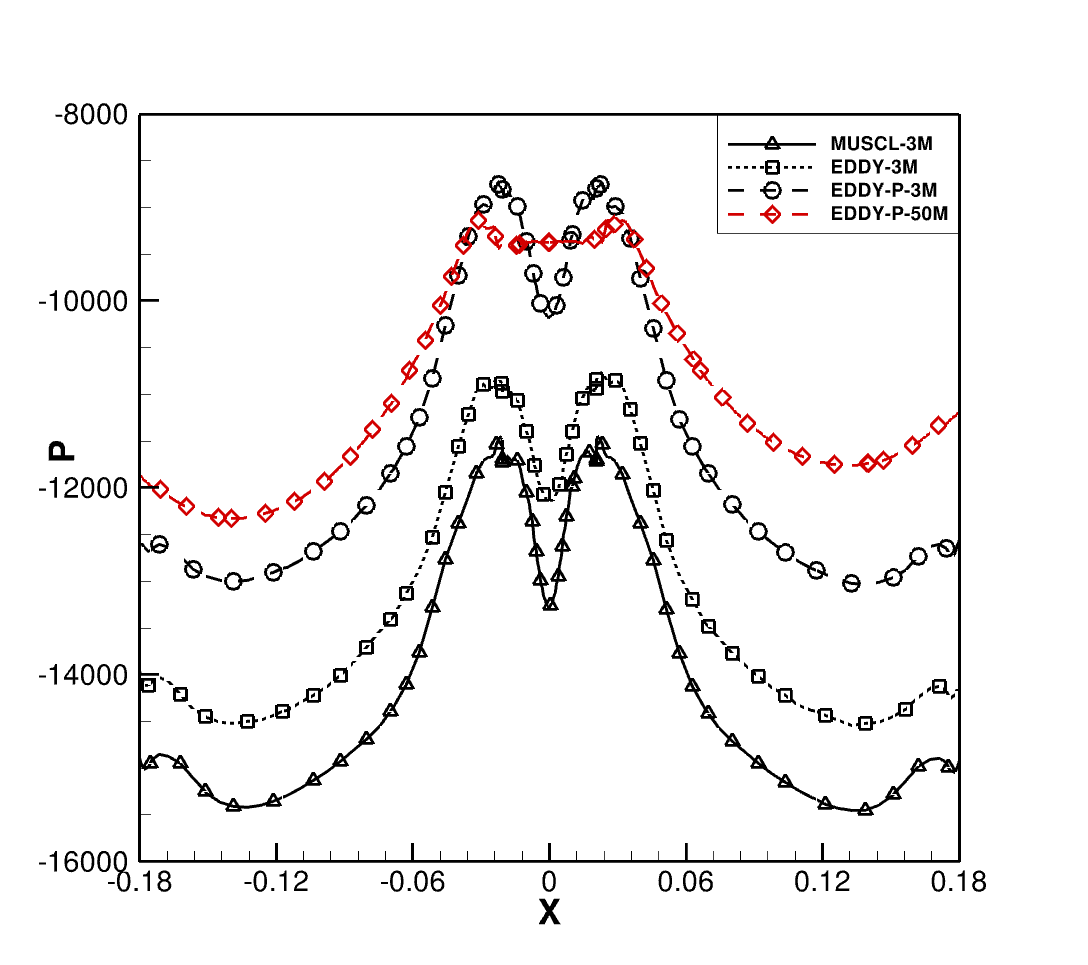
\includegraphics[clip=true, trim= 1.0cm 1.0cm 3.25cm 3.25cm,width=0.98\linewidth]{./figures/bulbt/P/3m}} \\             
     \subfigure[]{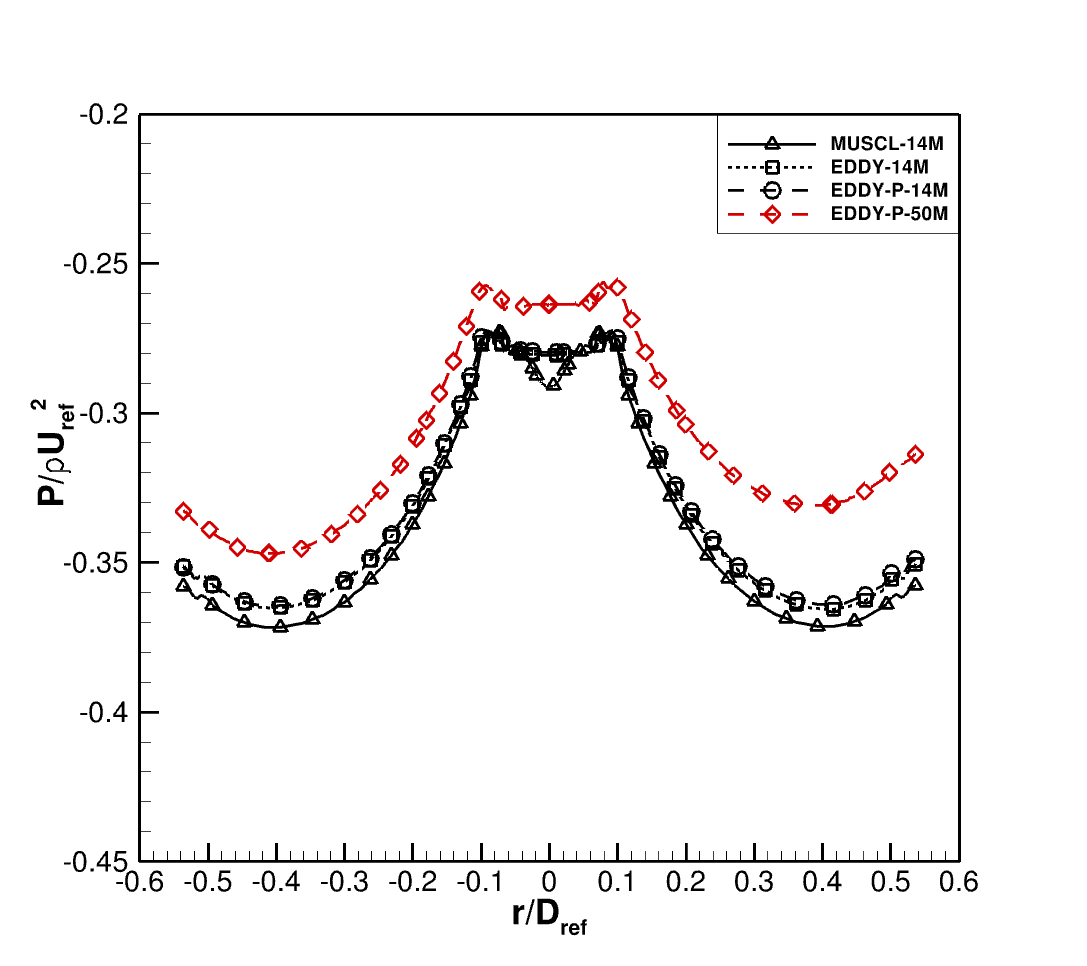
\includegraphics[clip=true, trim= 1.0cm 1.0cm 3.25cm 3.25cm,width=0.98\linewidth]{./figures/bulbt/P/14m}} \\
     \subfigure[]{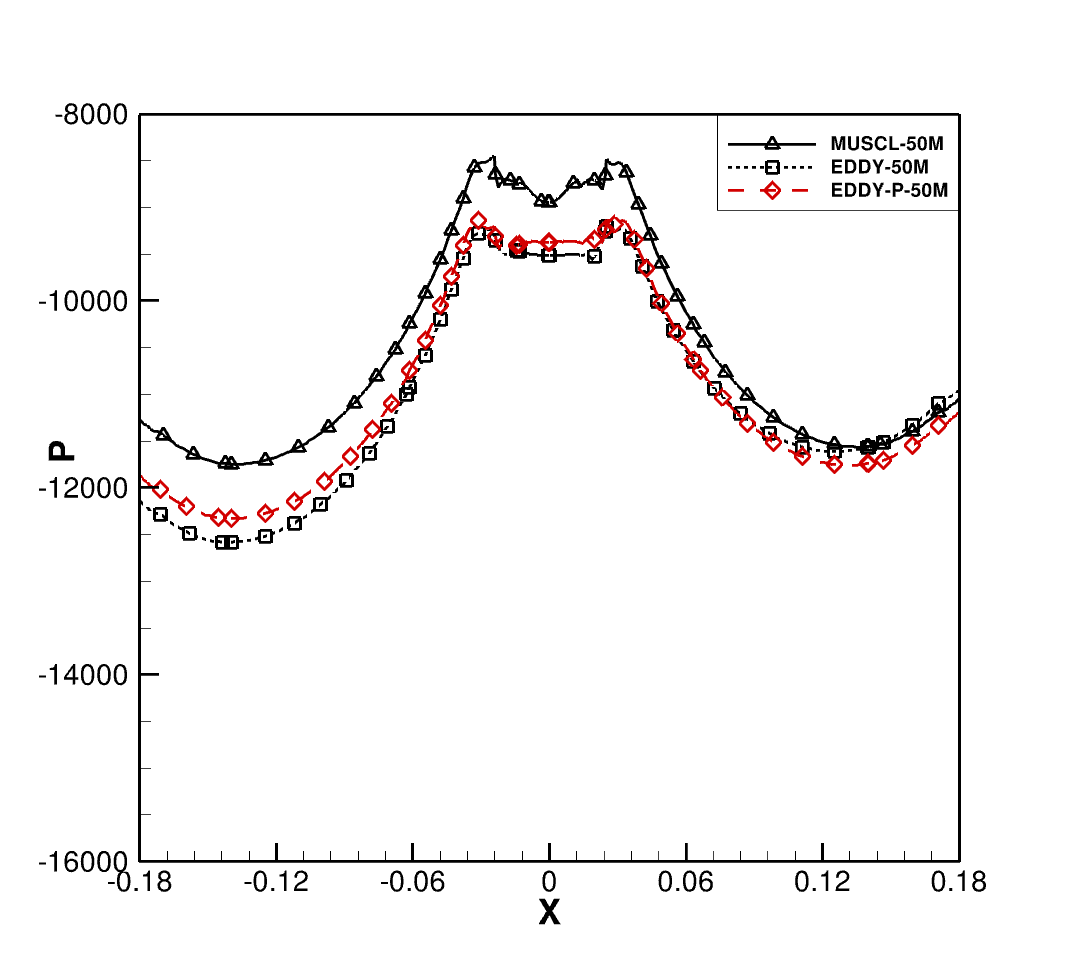
\includegraphics[clip=true, trim= 1.0cm 1.0cm 3.25cm 3.25cm,width=0.98\linewidth]{./figures/bulbt/P/50m}}     
     \caption{Pressure profiles at 4BY0 on (a)3M (b)14M (c)50M grid.}
     \label{p}            
\end{figure}
%%%%%%%%%%%%%%%%%%%%%%%%%%%%%%%%%%%%%%%%%%%%%%%%%%%%%%%%%%%%%%%%
%%%%%%%%%%%%%%%%%%%%%%%%%%%%%%%%%%%%%%%%%%%%%%%%%%%%%%%%%%%%%%%%
%\FloatBarrier
\begin{table}[t]
\caption{Relative $L^{2}$ norms of difference for pressure profiles.}
\begin{center}
\label{table2}
\begin{tabular}{c l l l}
\hline
Scheme & 3M     & 14M    & 50M    \\ 
\hline
MUSCL  & 28.72\% & 9.53\% & 4.58\% \\ 
EDDY   & 21.05\% & 7.76\% & 1.66\% \\ 
EDDY-P & 7.50\% & 7.43\% & 0.00\% \\
\hline 
\end{tabular}
\end{center}
\end{table}
%%%%%%%%%%%%%%%%%%%%%%%%%%%%%%%%%%%%%%%%%%%%%%%%%%%%%%%%%%%%%%%%
%%%%%%%%%%%%%%%%%%%%%%%%%%%%%%%%%%%%%%%%%%%%%%%%%%%%%%%%%%%%%%%%
%%%%%%%%%%%%%%%%%%%%%%%%%%%%%%%%%%%%%%%%%%%%%%%%%%%%%%%%%%%%%%%%
%%%%%%%%%%%%%%%%%%%%%%%%%%%%%%%%%%%%%%%%%%%%%%%%%%%%%%%%%%%%%%%%
%%%%%%%%%%%%%%%%%%%%%%%%%%%%%%%%%%%%%%%%%%%%%%%%%%%%%%%%%%%%%%%%
%%%%%%%%%%%%%%%%%%%%%%%%%%%%%%%%%%%%%%%%%%%%%%%%%%%%%%%%%%%%%%%%
\begin{table}[t]
\caption{Recovery coefficients from the inlet to the outlet.}
\begin{center}
\label{rc}
\begin{tabular}{c l l l}
\hline
Scheme & 3M     & 14M    & 50M    \\ 
\hline
MUSCL  & 1.0580 & 0.9194 & 0.8479 \\ 
EDDY   & 0.9906 & 0.9035 & 0.8696 \\ 
EDDY-P & 0.9097 & 0.9074 & 0.8662 \\
\hline 
\end{tabular}
\end{center}
\end{table}


%%%%%
%{\color{red} A marked difference is noted on the 14M grid, where the trend towards an increasing axial velocity in the upstream direction until the centerline is reported in both the experimental data as well as the EDDY and EDDY-P schemes. It will be shown in the subsequent section that this is primarily due to the lower artificial dissipation within this region.}
%{\color{red} the EDDY and EDDY-P schemes predict better the location of the maximum velocity and the low and constant circumferential velocity within the inner co-rotating zone. Similar to that observed in the axis velocity distribution, both EDDY and EDDY-P begin to show the correct trends by the 14M grid.}





















